
\documentclass{themeensg}
\usepackage{color}
\usepackage{listings}

%---Texte en filigranne---
\SetWatermarkText{\textsc{Brouillon}}
%pour l'enlever : \SetWatermarkText{}
\SetWatermarkText{}

% mise en page no-stress
\renewcommand{\familydefault}{\sfdefault}
%-------------------------

%---Mes packages à moi---
%\usepackage{}
%------------------------

%---Mes raccourcis---
\newcommand{\transpose}[1]{{}^t \! #1}
\newcommand{\ensg}{\textsc{Ensg}}

\renewcommand{\author}{Vincent HEAU}

%--------------------

%---Paramètres du pdf---
    \hypersetup{
       backref=true,                           % Permet d'ajouter des liens dans
       pagebackref=true,                       % les bibliographies
       hyperindex=true,                        % Ajoute des liens dans les index.
       colorlinks=true,  %Colorise les liens : true pour version numérique, false pour version d'impression
       breaklinks=true,                        % Permet le retour à la ligne dans les liens trop longs.
       urlcolor= black,                         % Couleur des hyperliens.
       linkcolor= black,                       % Couleur des liens internes.
       bookmarks=true,                         % Créé des signets pour Acrobat.
       %bookmarksopen=true,                    % Si les signets Acrobat sont créés,
                                               % les afficher complètement.
       pdftitle={Rapport de stage pluridisciplinaire},                 % Titre du document.
                                               % Informations apparaissant dans
       pdfauthor={\author},                      % dans les informations du document
       pdfsubject={Rapport de stage}           % sous Acrobat.
    }

%-----------------------



%-------------------------------------------------------------

\setcounter{tocdepth}{2} %profondeur de la table des matières

\title{Diffusion web de la base de donnée topographique de la Polynésie Française}

\bibliography{latexppmd}

%
%-------------------------------------------------------------
% Début du document
%--------------------------------------------------------------
\begin{document}
%--------------------------------------------------------------
\begin{titlepage}
%Inclusion des labels des entreprises
%Pour un seul label (à gauche), mettre NULL pour les 3e et 4e argument
\enterprise 
{logos/logo_ensg}
{Ecole Nationale des Sciences Géographiques}
{logos/logo_daf_bis}
{Direction des Affaires Foncières de la Polynésie Française}
\vspace{1cm}
%Inclusion du titre

\maketitle{{Rapport de Projet Pluridisciplinaire}\\{Cycle des Ingénieurs  diplômés de l'ENSG 2\up{ème} année (IT2)}}{images/logos/accueil.png}


\infos{\author}{Août 2022}
\end{titlepage}


% ---Page du jury---
%---Page du jury---
%\newevenpage
\thispagestyle{plain}
\section*{Jury}
\vspace{0.5cm}

\textbf{Président de jury :} \\

Jocelyne MARC

\vspace{0.5cm}

\textbf{Commanditaire :} \\

Direction des Affaires Foncières (DAF) de la Polynésie Française

\vspace{0.5cm}

\textbf{Encadrement de stage :} \\ 

Yoann RONCIN, Responsable de la cellule Topographie

\vspace{0.5cm}

\textbf{Enseignant référent :} \\ 

Emmanuel FRITSCH

\vspace{0.5cm}

\textbf{Rapporteur expert :} \\ 

qui est rapporteur du mémoire ?

\vspace{0.5cm}

\textbf{Responsable pédagogique du {\color{red} cycle Ingénieur} :} \\

Jean-François Hangouët, IGN/ENSG/DIAS

\vspace{0.5cm}

\textbf{Gestion du stage :} \\ 



\vspace{0.5cm}


\copyright \hspace{0.3cm} ENSG

\section*{Stage de fin d'étude du 23/05/2022 au 13/08/2022}
\vspace{0.3cm}
\textbf{Diffusion web :} $\boxtimes$ Internet \hspace{0.2cm}$\boxtimes$ Intranet Polytechnicum\hspace{0.2cm}
$\boxtimes$ Intranet ENSG\vspace{0.3cm}

\textbf{Situation du document :} 
\vspace{0.2cm}
\par
Rapport de stage pluridisciplinaire présenté en fin de 2\up{ème} année du cycle des Ingénieurs
\vspace{0.3cm}


\newcounter{x}
\setcounter{x}{\getpagerefnumber{LastPage}-\getpagerefnumber{beginappendices}+1}

\textbf{Nombres de pages :} \getpagerefnumber{LastPage} pages dont \arabic{x} d'annexes
\vspace{0.3cm}

\textbf{Système hôte :} \LaTeX
\vspace{1cm}


\textbf{Modifications :} 
\begin{center}
\begin{tabular}{|c|c|c|>{\centering}p{6.5cm}|}
\hline 
EDITION & REVISION & DATE & PAGES MODIFIEES\tabularnewline
\hline
\hline 
1 & 0 & 09/2016 & Création\tabularnewline
\hline 

\end{tabular}
\end{center}
%------------------

%------------------------------------------------------------------------------
% Remerciements
\newevenpage
\chapter*{Remerciements}
\begin{comment}
Ce stage au sein de la Direction des Affaires Foncières de la Polynésie Française a été une expérience professionnelle particulièrement enrichissante. Je tiens à remercier mes collègues de travail de la cellule Cadastre-Topographie, Lucie, Frédéric, Tania, Mira, Maud et François pour m'avoir permis de m'intégrer au mieux et pour les moments passés ensembles. Je remercie Lucas, Matthieu, et Bernard de la cellule topographie qui, toujours avec beaucoup de gentillesse, ont pris le temps de regarder mes cartes, de me faire des retours et de m'aider. L'ambiance de travail au sein de la section Cadastre-Topographie est excellente et ces trois mois de travail furent très agréables. 
Je tiens à remercier tout particulièrement mon maître de stage Yoann RONCIN pour tout le temps qu'il m'a accordé, pour les conseils et toutes les compétences qu'il m'a permis d'acquérir que ce soit avec ArcGIS, ArcGIS Online ou encore FME . Grâce à lui, ce stage s'est avéré être extrêmement enrichissant et je suis heureux d'avoir pu découvrir et apprendre autant de choses grâce à lui.
Ce stage n'aurait pas été possible sans Alexandre AMARY, qui m'a proposé de m'accueillir à la DAF pour travailler sur un sujet qui m'a beaucoup plu. Je le remercie sincèrement.

Enfin, je souhaitais aussi remercier mon professeur référent Emmanuel FRITSCH pour ses commentaires et ses retours constructifs ainsi que Cécile DUCHENE, qui bien que n'étant pas mon professeur référent, a pris le temps de m'écrire, de me proposer son aide et de m'envoyer des documents concernant la généralisation qui se sont avérés particulièrement utiles lors de la rédaction de mon rapport. 
 
\end{comment}

%---Résumé (français)---
\begin{abstract}
\thispagestyle{empty}
	\vspace{1cm}

	
En Polynésie Française, les données cartographiques sont mises à disposition et maintenues par la section Cadastre-Topographie de la Direction des Affaires Foncières (DAF). Jusqu’à présent la donnée cartographique était collectée au 1/5 000e et symbolisée à des échelles destinées à l’impression papier: 1/5 000e, 1/15 000e, 1/25 000 et 1/50 000e sans travail de généralisation cartographique. Ce projet a vocation à être un travail expérimental destiné à mettre en place un fond de carte topographique approprié à une utilisation multi échelle sur le web et à l’utiliser au sein d’applications web similaires au géoportail. Le travail préliminaire a nécessité une généralisation cartographique aux multiples échelles choisies. En vue de produire des cartes cohérentes à diverses échelles, cette généralisation s'accompagne d'un travail d'étiquetage et de symbologie. La généralisation permettra de rendre le portail plus interactif et plus clair pour la visualisation de la Polynésie à toutes les échelles et non plus seulement au 1/5000. C'est une phase primordiale permettant non seulement une navigation fluide de l'utilisateur lors du changement d'échelle, mais aussi une cartographie lisible et adaptée aux différents niveaux de zoom. Pour parvenir à ce résultat, une importante préparation des couches est nécessaire en effectuant pour chacune d'entre elle, les traitements adaptés. La finalité de ce travail préparatoire est la publication sur le web à l'aide d'ArcGIS Online, ainsi que l'utilisation du portail à travers diverses thématiques comme la diffusion des fiches géodésiques et de nivellement.

	\vspace{1.5cm}
	
	\textbf{Mots clés :} Fond de carte, généralisation cartographique, symbologie, étiquetage, cartographie web, Polynésie Française
\end{abstract}
%-----------------------
\begin{comment}

\end{comment}

%---Résumé (anglais)---
%\selectlanguage{english}
\begin{abstract}
\thispagestyle{empty}
	\vspace{1cm}
	
	\begin{comment}
 	This project is willing to produce a web cartography of French Polynesia based on the topographic data of the [DAF]. Map production at such diffrent levels could not be realised without cartographic generalization as well as labeling and symbology. This preliminary work aims not only at producing maps able to fit the selected scale on a web plateform, but also at improving the changes of scales to make it easy to read and understand.
	This part is fundamental and should be done throughout many algorithms able to transform data produced for 1:5000 map. The purpose is to produce a web portal which will also be used to broadcast geodesic sheets.
   \end{comment}

	\vspace{1.5cm}
	
	\textbf{Key words:} Basemap, cartographic generalization, symbology,labeling, web cartography, French Polynesia
	
\end{abstract}
%----------------------

\selectlanguage{french}

%---Table des matières, des figures et des tableaux---
\newevenpage
\tableofcontents



\newevenpage
\chapter*{Glossaire et sigles utiles}
\addcontentsline{toc}{chapter}{Glossaire et sigles utiles}

  \begin{acronym}
  \acro{ENSG}{\'Ecole Nationale des Sciences Géographiques}
  \acro{DAF}{Direction des Affaires Foncières - La cellule topographie, rattachée à la section Cadastre-Topographie de la DAF a notamment pour mission la cartographie de la Polynésie}
  \acro{SGBD}{}
  \acro{BDG}{}
  \acro{BDC}{}
  
  \acro{PAI}{Points d'activité et d'intérêt - Correspondent à une catégorie particulière en cartographie}
  \end{acronym}

\begin{comment}

\begin{center}
    \textbf{Vocabulaire de la cartographie en Polynésie Française}\\
    \vspace{0,25cm}
    \textit{La cartographie en Polynésie Française nécessite l'utilisation de mots en tahitiens ou de mots spécifiques au lexique des îles entourées de lagon du Pacifique . Ci-dessous, ce glossaire présente quelques termes utiles à la lecture et à la compréhension des cartes polynésiennes. Certains mots sont illustrés par les figures de la page suivante.}
\end{center}

 \begin{acronym}
 
 \acro{Hoa}{Mot tahitien désignant une petite ouverture de la barrière de corail sur la mer semblable à une petite passe de faible profondeur.}
 
 \acro{Maoti}{Nom tahitien désignant une résurgence du récif au large. Les Maoti sont souvent très visibles lors des fortes houles, lorsque les vagues y déferlent.(Ils s'observent notamment sur la côte est de Tahiti)}
 
 \acro{Marae}{Lieu de culte des anciens polynésiens, caractérisés aujourd'hui comme des points d'activité et d'intérêts}
 
  \acro{Motu}{Un motu est un îlot corallien qui apparaît dans le lagon à la suite d'une accumulation du récif barrière. La formation d'une lentille d'eau douce en dessous du Motu permet à un certain type de végétation de s'y développer. Certains motus sont célèbres comme le Motu Uta de Papeete sur lequel à été installé le port industrielle, le stockage du pétrole ou encore le dépot des conteneurs.}
  
  
  \acro{PK}{Point kilométrique - Bornes kilométriques caractéristiques en Polynésie française et permettant de se repérer notamment sur l'île de Tahiti}
  
  \acro{PK}{Point kilométrique - Bornes kilométriques caractéristiques en Polynésie française et permettant de se repérer notamment sur l'île de Tahiti}
  

  \end{acronym}


\begin{figure}
\centering
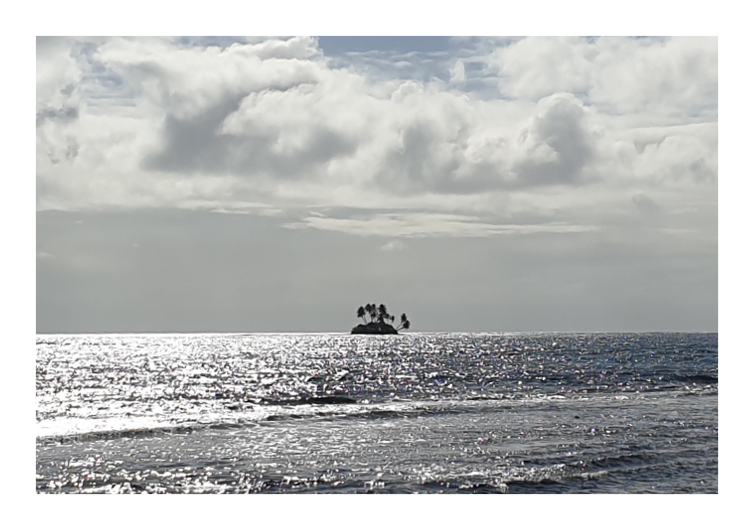
\includegraphics[width=\linewidth]{images/Annexes/nono.png}%
\caption{Motu Nono au large d'Afaahiti}%
\label{fig:graphics}% label for figure
\end{figure}

\begin{figure}
\centering
\subfloat{\label{fig:gull}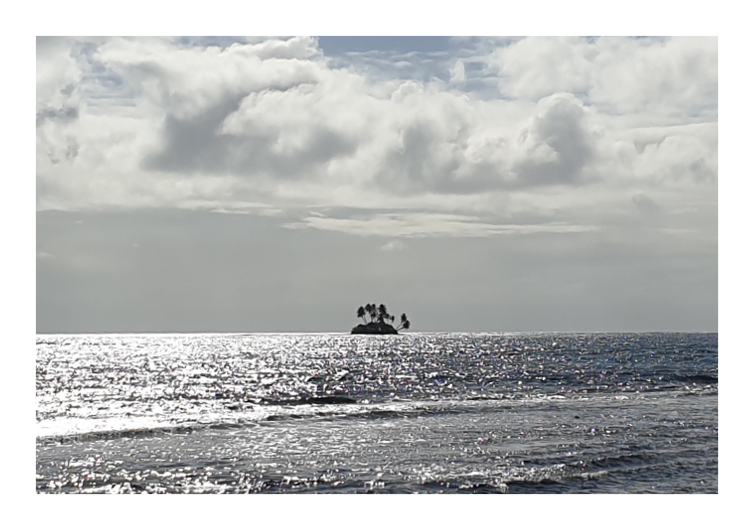
\includegraphics[width=0.4\textwidth]{images/Annexes/nono.png}}
\subfloat{\label{fig:tiger}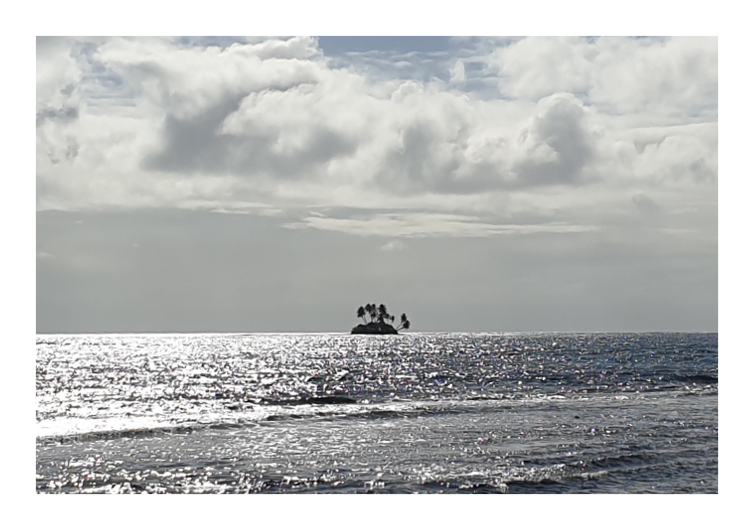
\includegraphics[width=0.4\textwidth]{images/Annexes/nono.png}}
\subfloat{\label{fig:mouse}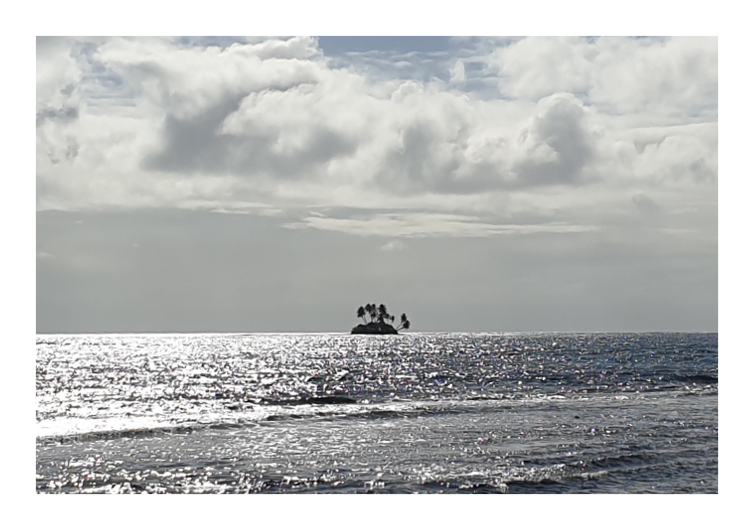
\includegraphics[width=0.4\textwidth]{images/Annexes/nono.png}}
\subfloat{\label{fig:mouse}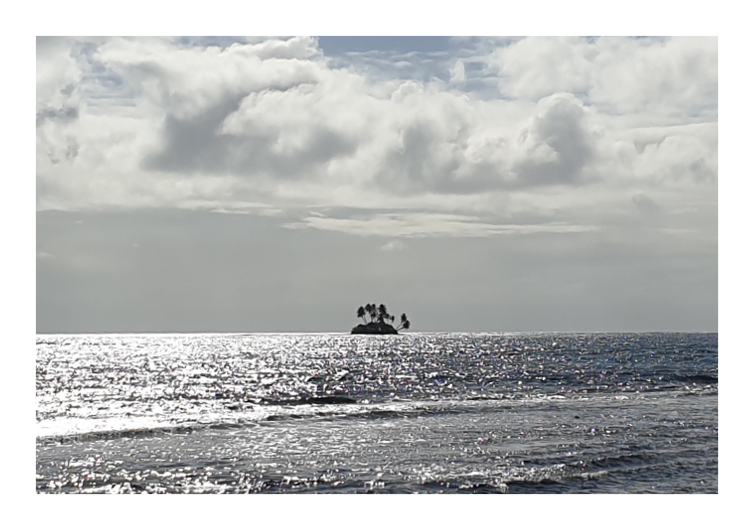
\includegraphics[width=0.4\textwidth]{images/Annexes/nono.png}}
\caption{Mettre les figures utiles et correctement et au cas où...}
\label{fig:animals}
\end{figure} 


\end{comment}
%---Introduction------------------------------------------------------------------
\newevenpage
\chapter*{Introduction}
  \addcontentsline{toc}{chapter}{Introduction}
  
  \vspace{1.5cm}
	Cartographier la Polynésie Française, c'est cartographier un espace vaste de 4167 km², équivalent à la superficie de l’Europe. C'est la mission de la Direction des Affaires Foncières de la Polynésie Française et plus particulièrement celle de la section cadastre-topographie, qui est l'une des quatre grandes divisons de la DAF. Deux géomaticiens, deux géomètres et un aide technique travaillent au sein de la cellule topographie et maintiennent et mettent à jour les données. Elles sont d'une grande précision et disponibles pour l'ensemble des îles de la Polynésie Françaises mais ne sont adaptées que pour une cartographie à l'échelle 1/5000. La DAF propose dans un catalogue, de nombreux produits cartographiques sur demande des utilisateurs mais il n'existe pas à l'heure actuelle de généralisation globale de cette base de données pouvant servir à la cartographie web.
	
	Avec l'essor des plateformes de type "Géoportail", la demande en cartographie web est forte. L'objectif de ce stage est de réaliser un travail préparatoire et exploratoire dans ce domaine pour fournir une première version d'un fond de carte adapté à un géoportail. L'ensemble des traitements effectués servant à généraliser les couches, ainsi que l'étiquetage et la symbologie proposée serviront donc de base pour la cellule topographie de la DAF qui pourra s'appuyer sur ce travail par la suite. Ce projet se compose donc de plusieurs phases de travail permettant d'aboutir à une diffusion via ArcGIS Online des données. Il répond à la problématique de diffuser sur le web un portail cartographique spécifique à la Polynésie Française.
	
	Les grands axes de ce rapport suivent le déroulement du projet. Il s'agira d'abord de prendre en main l'architecture de la base de données puis de choisir une gamme d'échelles. Ensuite, ce rapport évoquera les traitements spécifiques à chaque couche via des logiciels comme ArcGIS Pro ou FME. Puis le projet se poursuivra par une phase de cartographie sur ArcGIS PRO nécessitant la mise en place d'un étiquetage, d'une symbologie ainsi que l'ajout de raster permettant l'habillage de la carte. Ces phases préparatoires conséquentes, qui constituent la plus grande partie du travail réalisé, permettront de disposer d'une gamme de cartes adaptées à des échelles variées. Cependant, leur diffusion web, qui correspond au dernier axe de travail nécessite une restructuration pour faire face aux contraintes de l'export qui seront détaillées dans ce rapport. La diffusion web via ArcGIS Online sera l'occasion de décliner le portail à diverses utilisations, notamment au travers d'une application web destinée à la diffusion des fiches géodésiques et de nivellement. 
  
  \begin{comment}
  \begin{figure}[ht]
\centering
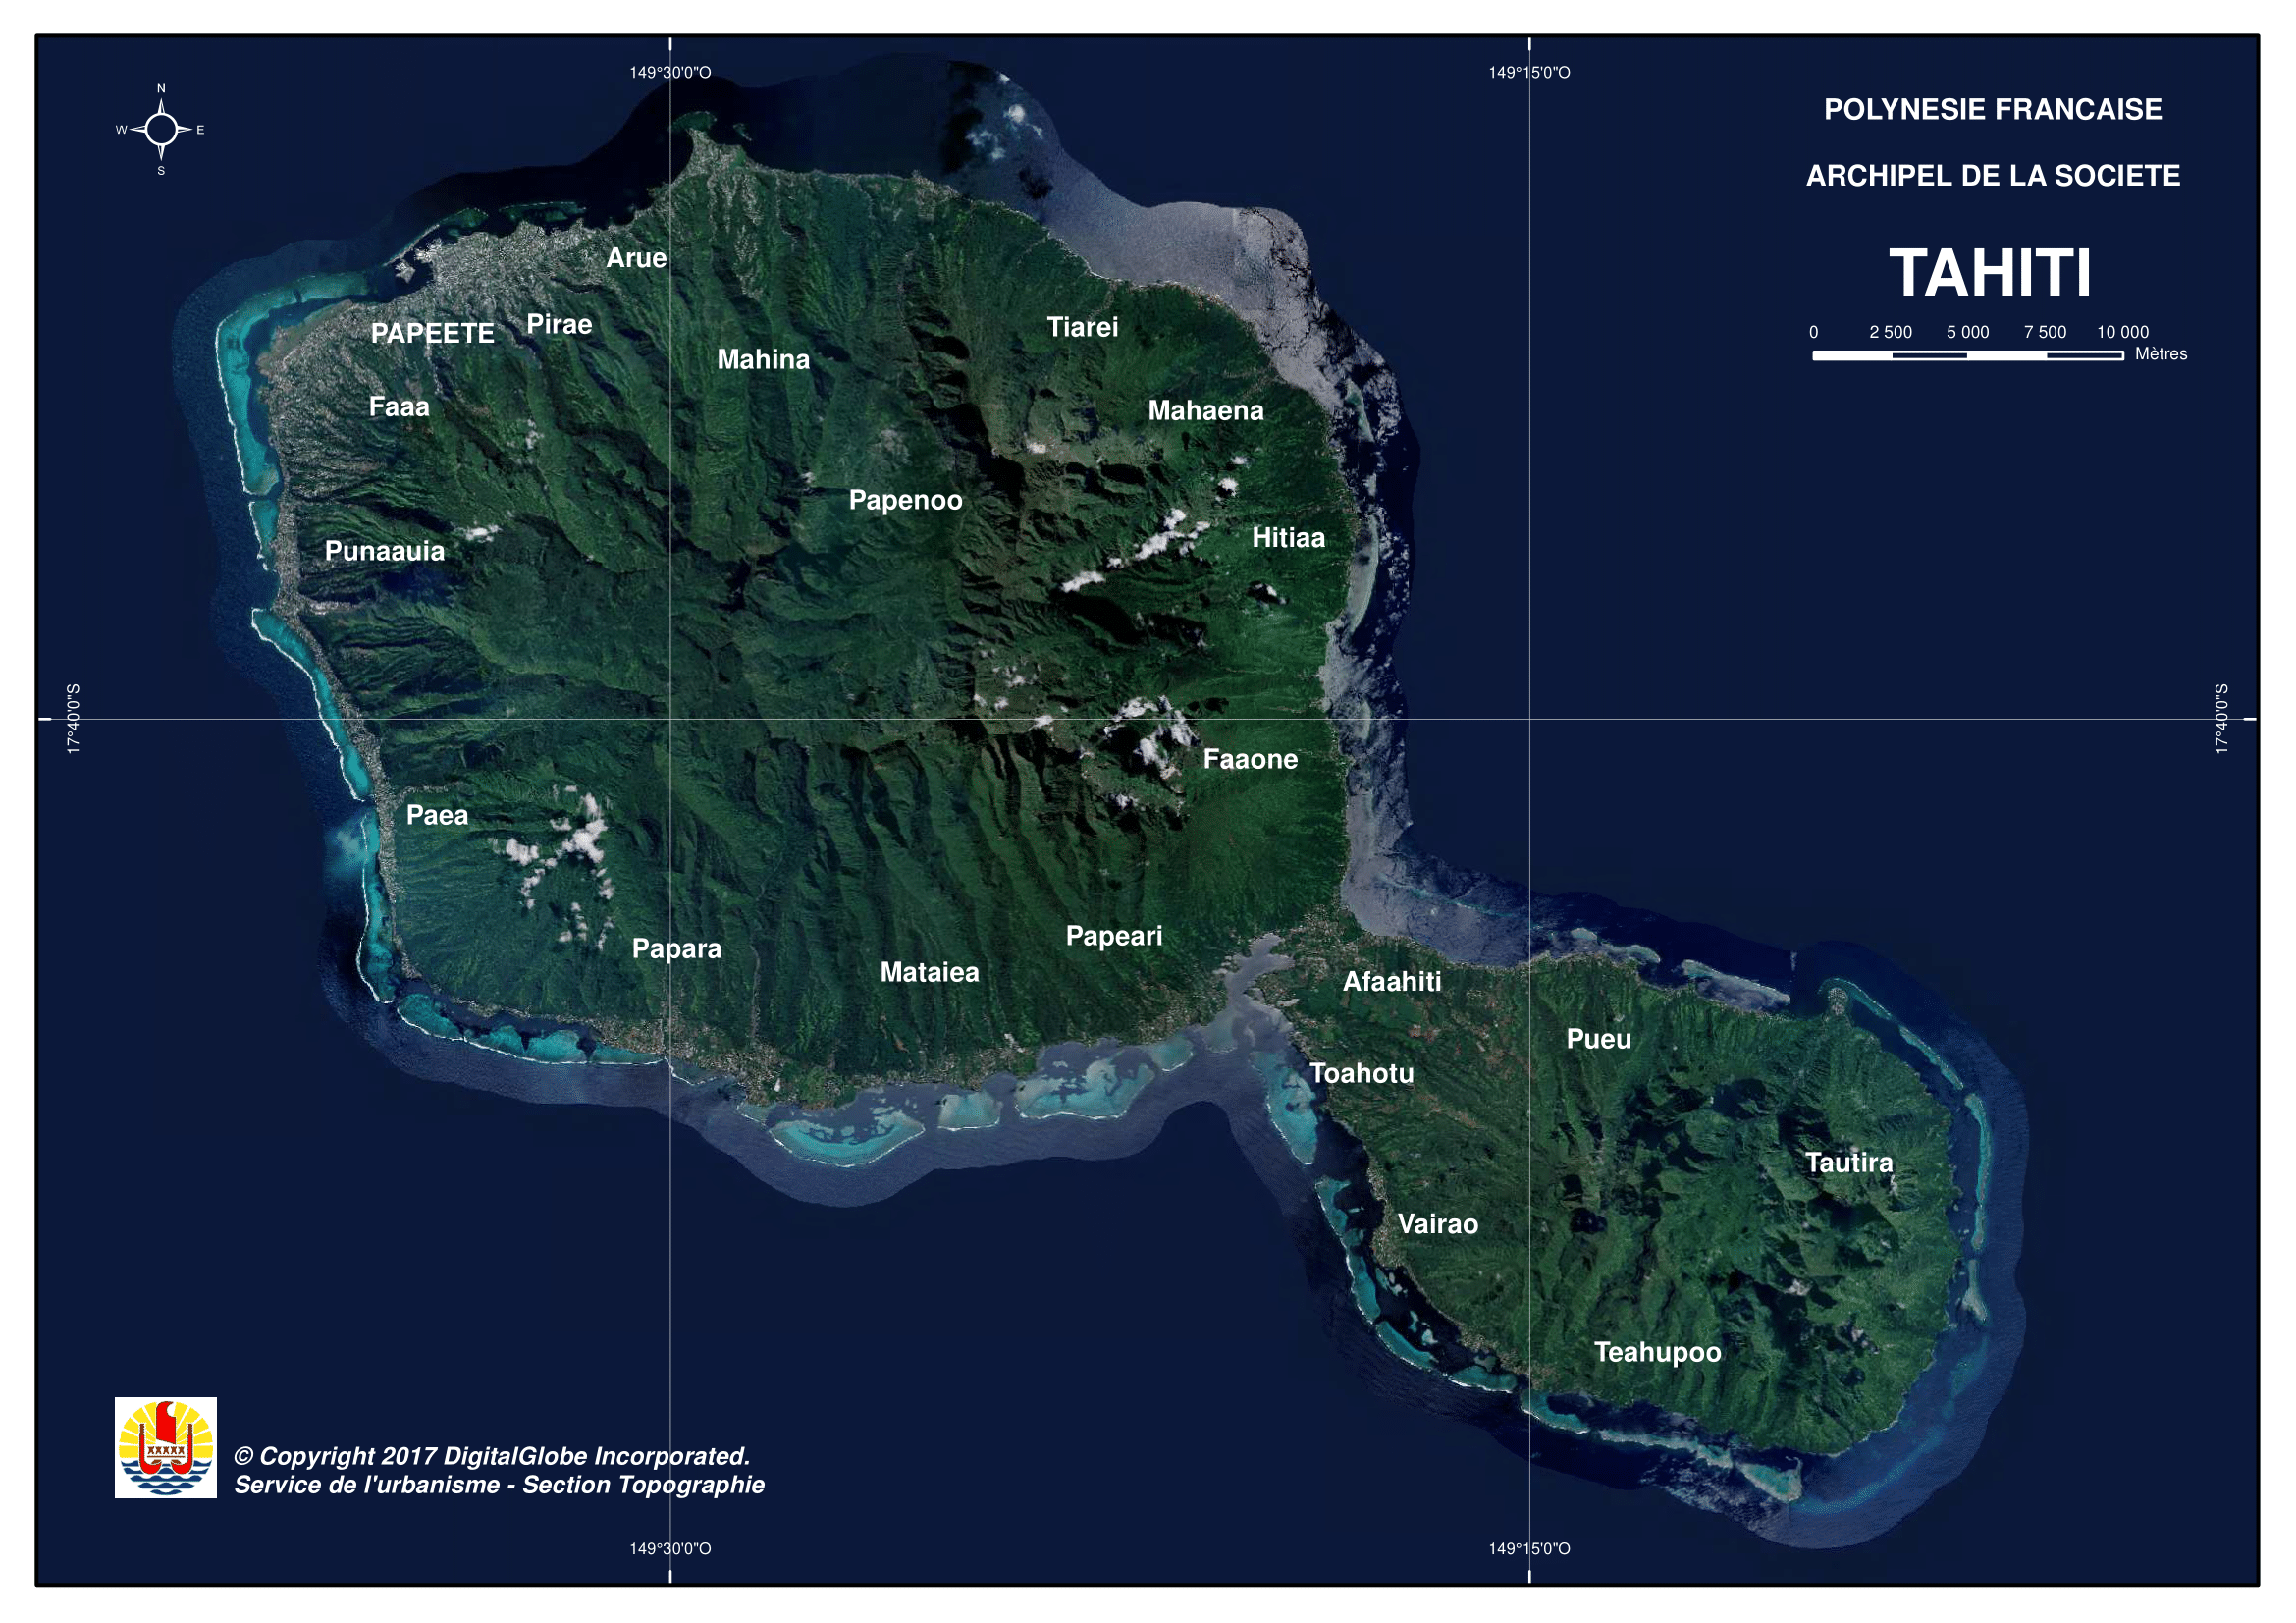
\includegraphics[width=12cm]{images/Annexes/Photoplan_Tahiti_2017_A4_paysage_1-1.png}
\caption{Exemple de produit réalisé par la DAF}
\label{intro}
\end{figure}
  \end{comment}
    

%-------------------------------------------------------------------------------


\evenchapter{Diagnostic de la base de donnée topographique et cadre de travail}

\textit{Les produits cartographiques maintenus par la DAF sont les données sur lesquels porte le travail de ce stage. Cette partie s'attarde donc à les présenter et à les expliciter. La notion de généralisation et son cadre d'utilisation est elle-aussi précisée.}
 
\section{La cellule topographie de la Direction des Affaires Foncières}

\subsection{Organisation de la cellule topographie}
La cellule topographie est une cellule de la section Cadastre-Topographie qui est l'une des quatre sections de la Direction des Affaires Foncières de la Polynésie Française. Les grandes missions de ce service sont équivalentes à celles de l'IGN en métropole avec la cartographie de la Polynésie Française, l'acquisition des données ainsi que la maintenance et la densification des réseaux géodésiques et de nivellement. Ces missions sont assurées par des géomètres-cartographes et des géomaticiens qui travaillent au sein de cette cellule. 

\subsection{Produits cartographiques maintenus}
La section topographie propose de nombreux produits et prestations qu'il est possible de passer en revue dans un catalogue dédié. Il est disponible sur le site internet de la DAF [https://www.service-public.pf/daf/]. Parmi les produits cartographiques, on trouve notamment :

\begin{itemize}
\item \textbf{Des cartes et des plans } - Deux types de cartes sont proposées. La première catégorie est celle de la carte topographique de référence ( la carte au 1/5000 couvre Tahiti en 81 planches) . A Tahiti, des éditions au 1/2000 sont également disponibles sur la zone urbaine. La seconde catégorie est la carte de type \textit{CARTO ILE} avec des éditions aux 1/25000 ou 1/50000 produites sur demande en cartes papier et en dalles au format numérique jpg géoréférencé sans toutefois que les couches qui composent ces cartes ne soient réellement généralisées.
\item \textbf{Des données topographiques} parmi lesquelles on retrouve une BD Topo administrée par le SGBD PostGreSQL/PostGIS  et dont l'architecture fait l'objet de la sous-partie suivante. Les données sont en libre accès comme c'est le cas pour les produits MNT.
\item \textbf{Des photoplans et spatio-cartes} produites à partir des photographies aériennes et des photos d'archives dont la section topographie est détenteur d'une vaste collection.
\end{itemize}

Par ailleurs, une mission de ce service est la maintenance d'un vaste réseau de repères géodésiques et de nivellement utilisables par les entreprises qui peuvent avoir accès aux fiches signalétiques des repères.


\subsection{Méthodes d'acquisition de la donnée}
La création de l'ensemble de ces produits cartographiques se fait principalement par prise de vue aérienne ou satellitaire et est soumise à des obstacle météorologiques. En effet, la présence de nuage quasi-permanent en zone montagneuse rend les acquisitions difficiles. Seules certaines périodes de l'année et à des horaires bien précis sont propices aux prises de vue.  On constate cela notamment en comparant les MNT mondiaux à ceux réalisés par la section Topographie. La figure \ref{ombrage} le démontre particulièrement sur les sommets montagneux où les données d'Esri sont incomplètes en raison de la forte couverture nuageuse.
\begin{figure}[ht]
\centering
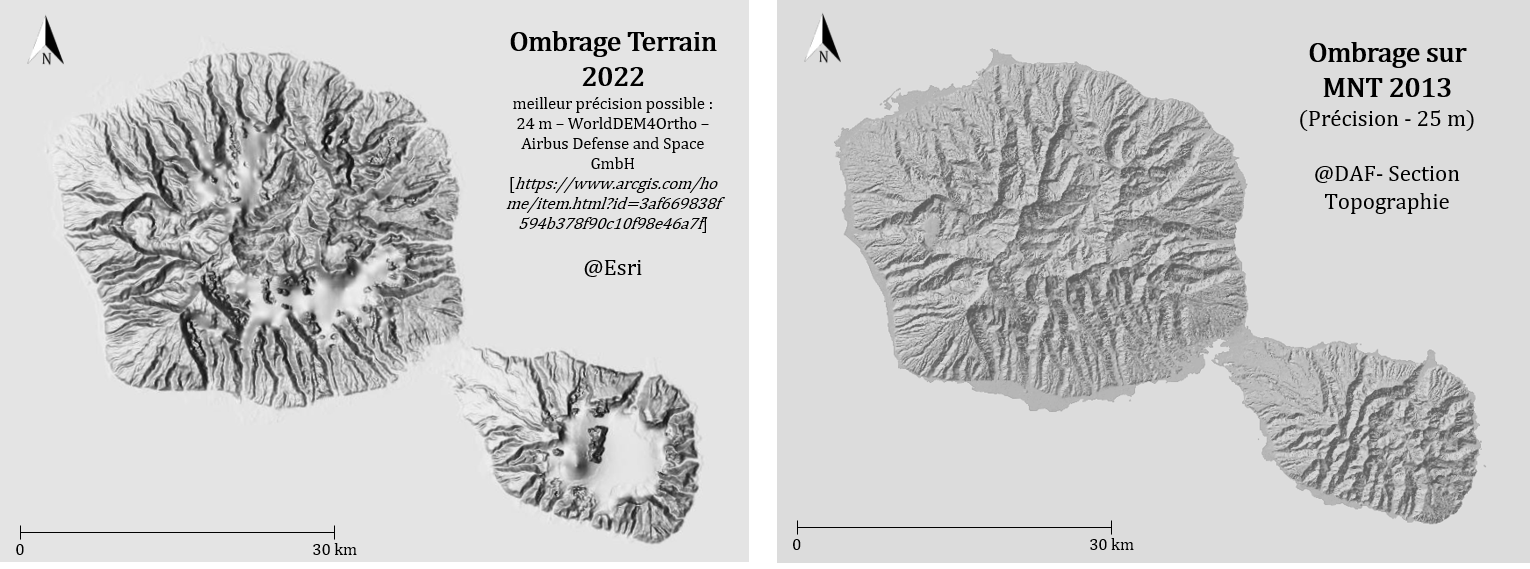
\includegraphics[width=\linewidth]{images/chap0/ombrage}
\caption{Comparaison des ombrages issus de deux sources différentes - Tahiti}
\label{ombrage}
\end{figure}

\section{Architecture de la base de données topographique de la Polynésie Française}

\subsection{Classes d'entités composant la base}

\begin{figure}[ht]
\centering
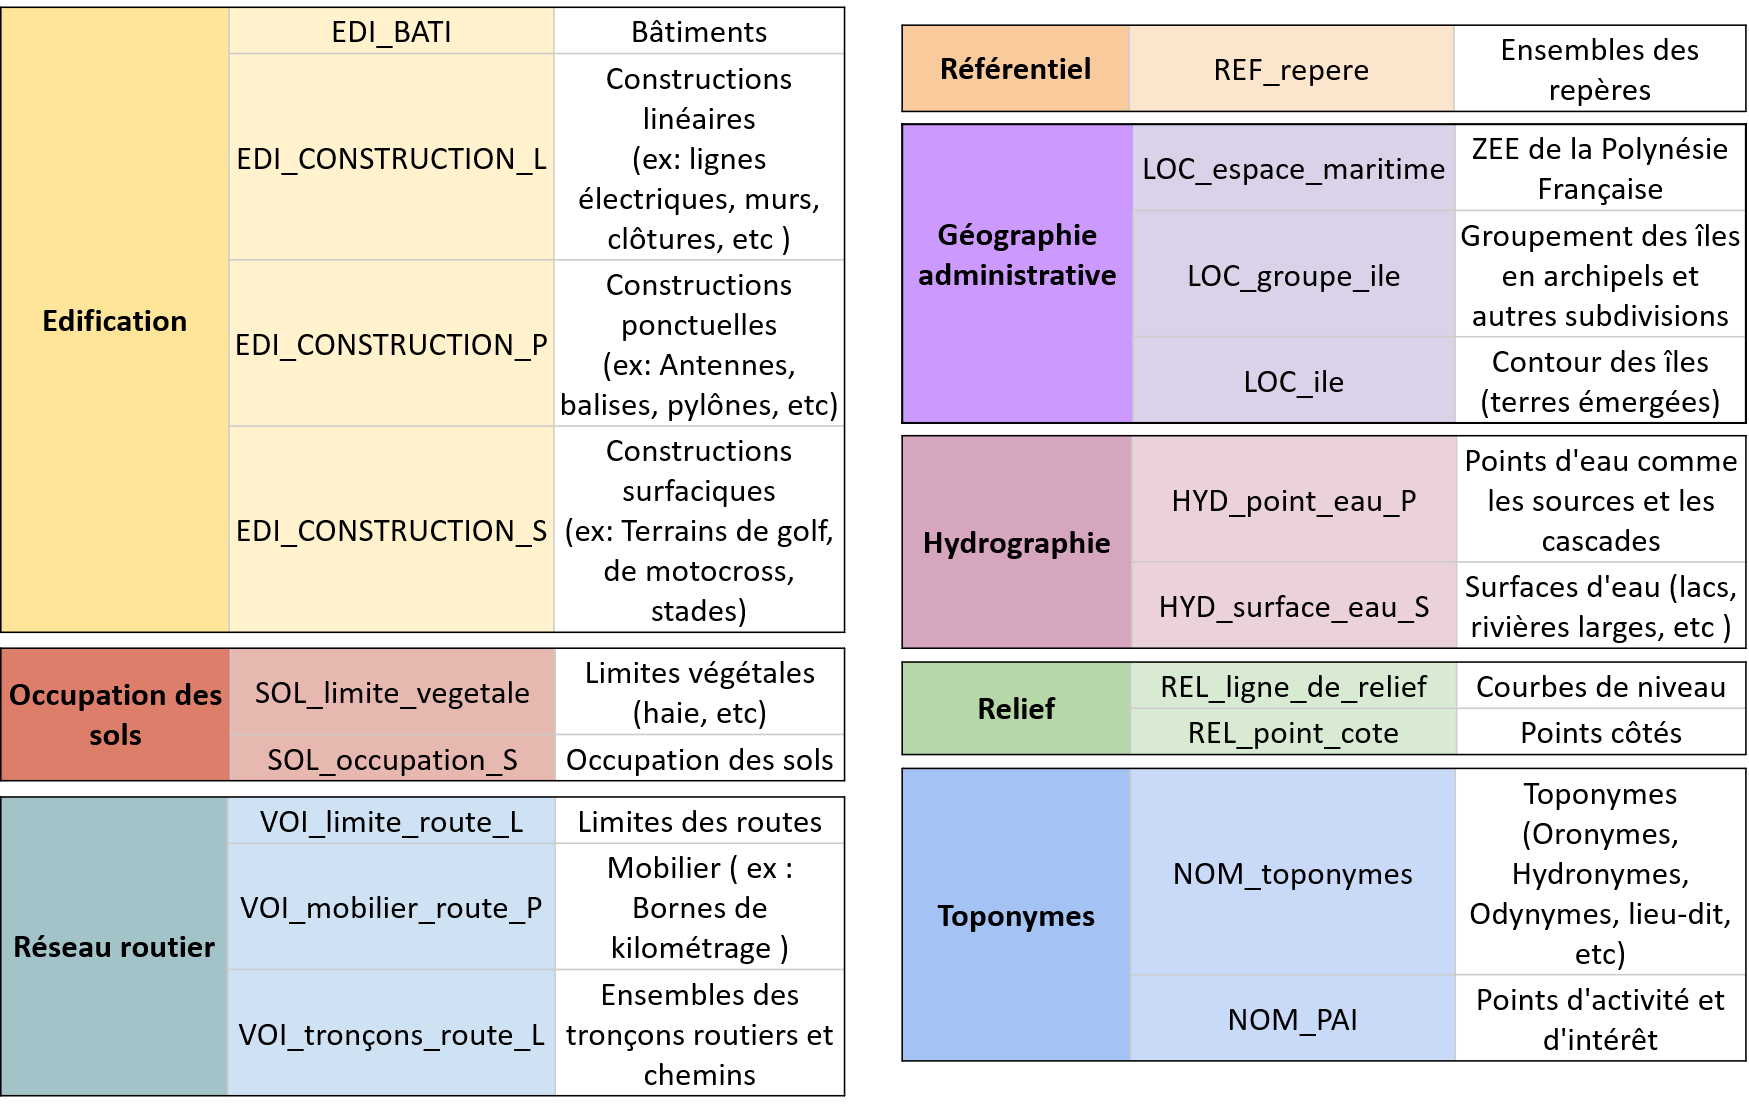
\includegraphics[width=12cm]{images/chap1/bd_simplifie.png}
\caption{Représentation simplifiée de la base de donnée de la DAF - Liste des classes du diagramme de classe la schématisant (groupement par thématique)}
\label{bd_simplifie}
\end{figure}
Les données produites par la DAF et servant à la cartographie figurent dans une base de donnée mise à jour régulièrement. C'est une \textit{base de donnée géographique}. Ce terme sera précisé dans le chapitre suivant. En effet, nous distinguerons les différentes généralisations possibles ainsi que les différents types de bases de données qui en découlent. 

De nombreux objets sont répertoriés dans la base qui s'articule en 31 classes. La figure \ref{bd_simplifie} présente une représentation schématique et simplifiée de la base de donnée faisant figurer uniquement les classes qui participent directement à la production des cartes. Une liste plus détaillée de l'ensemble des classes avec leurs détails fait l'objet de l'annexe B tandis que le diagramme UML complet de cette base de donnée figure en annexe A. On y retrouve l'ensemble des classes avec notamment les catégories et sous-catégories pour chacune d'entre elles. Pour celles qui présentent une représentation graphique, cette catégorisation est à l'origine de la symbologie.

\subsection{Répartition en quatre fuseaux UTM}
{\color{magenta} NON REDIGE : Explication de la séparation de la base en 4 fuseaux UTM + carte à mettre représentant ces fuseaux (ici ou en annexe en fonction de la place)}

\begin{figure}[ht]
\centering
\includegraphics[width=\linewidth]{images/chap0/PF_carte_generale_UTM_90x90_2012-1.png}
\caption{Carte des fuseaux UTM - Produit de la section topographie - 2012}
\label{fuseauUTM}
\end{figure}

\section{Pré-requis pour la généralisation }
\textit{L'objectif de ce travail est donc de produire des cartes qui seront réalisées avec l'outil ArcGIS. Pour parvenir à réaliser une carte multi-échelles, des traitements de généralisation doivent être effectués sur chaque gamme d'échelle. Cette sous-partie précise le terme de généralisation cartographique ainsi que les ensembles de définition choisies pour ce projet.}
\subsection{Généralisation cartographique}
Il est nécessaire de commencer ce rapport en précisant certains adjectifs qui peuvent qualifier une base de données. La base de données de la DAF dont le diagramme de classe (annexe ??) a été présenté précédemment est une \textbf{base de données géographique} Comme le fait Marion Dumont \cite{Dumont2018}, nous ferons la distinction dans ce rapport entre une base de données géographique (BDG) et une base de données cartographique (BDC) dont l'utilisation est exclusivement liée à la représentation graphique. De plus, nous distinguerons \textit{la généralisation de modèle} visant à restructurer la BDG, la \textit{généralisation graphique} visant simplement à "respecter les contraintes de lisibilité" et enfin la généralisation cartographique. La généralisation cartographique, le coeur du travail durant ce stage, est le processus qui permet de produire des cartes à différentes échelles à partir de la BDG. La figure \ref{dumont} issue de la thèse de Marion Dumont permet comprendre ces termes.

\begin{figure}[ht]
\centering
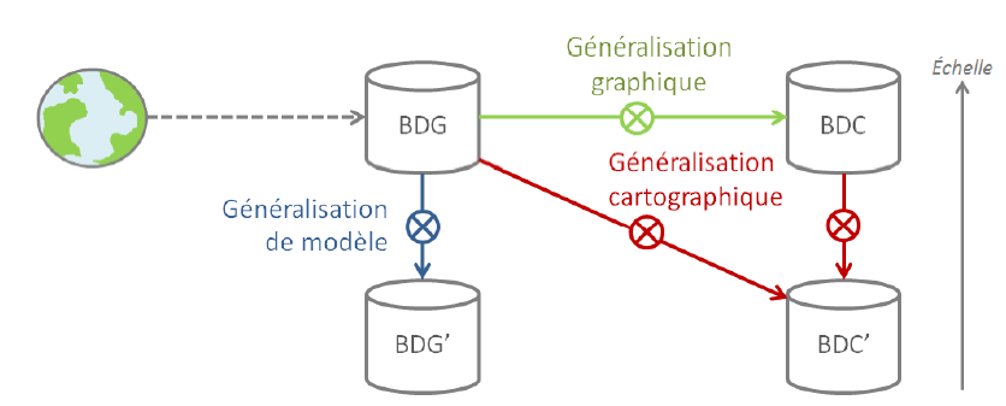
\includegraphics[width=\linewidth]{images/chap1/generalisation_dumont.png}
\caption{Les différents types de généralisation}
\label{dumont}
\end{figure}
Disposant à la fois de la base de donnée BD TOPO de la DAF ainsi que du projet type de cartographie à l'échelle 1/5000, il s'agira donc de mettre en place des traitements permettant de réaliser la cartographie non plus seulement au 1/5000 mais à des échelles inférieures. Par ailleurs le choix des échelles de travail, effectué en début de stage sera justifié plus loin.

L'objectif est d'obtenir un panel de cartes aux échelles choisies. Le travail préliminaire à la diffusion web se décompose en deux phases qui font chacune l'objet d'un chapitre de ce rapport. La première partie est une généralisation cartographique accompagnée de la production des métadonnées associées. Pour chacune des échelles, la BDG de départ sera adaptée pour fournir une BDC en accord avec l'échelle (notée BDC' sur la figure 1.4). Ensuite, le travail se poursuivra pour réaliser la cartographie à partir de cette base de donnée. L'étiquetage, l'habillage de la carte avec des fonds rasters et le choix de la symbologie feront l'objet de cette partie. Il faut noter que la première phase amènera à discuter de la structure de la BDG, que ce soit la pertinence de certains champs ou encore la nécessité d'en créer de nouveaux.

%Enfin, bien qu'il ne s'agisse que d'un travail préparatoire qui a vocation à évoluer, la perspective de la diffusion web doit être envisagée dès les premiers traitements. 

%Aux conseils du maître de stage, s'ajoutent les recommandations trouvées dans les travaux de Marion Dumont \cite{dumont}. En effet sa thèse évoque la généralisation et la fluidification des transitions entre les différents niveaux de zoom.

Au regard de cette analyse, de nombreuses questions surviennent notamment quant au choix des échelles et de la zone de travail.

\subsection{Choix des échelles}
Durant ce stage, la généralisation s'est portée sur huit niveaux d'échelle. La plus grande échelle\footnote{La question d'échelle est au coeur du processus de généralisation, et dans ce rapport, nous utiliserons souvent les termes "grande échelle" ou "petite échelle". Ils  seront employés dans leur sens arithmétique. Ainsi, l'échelle 1/5000 du cadastre est une plus grande échelle que l'échelle 1/500 000 car le dénominateur du quotient est plus faible et donc la fraction est plus grande. C'est cette convention qui est notamment utilisée par ArcGIS dans la documentation. L'ENS Lyon et sa plateforme GéoConfluence propose une définition plus détaillée de l'utilisation du terme échelle en géographie }, le 1/5000 est déjà cartographiée. Un projet ArcGIS nommé \textit{"export\_topo\_5000"} a été fourni en début de stage. Ce projet comporte l'ensemble des couches utilisées, la symbologie et l'étiquetage adéquat pour cette échelle ainsi que les fonds raster ajoutés au projet. Il sert de modèle et le travail sera fait de manière à ce que l'utilisateur puisse zoomer progressivement et naturellement vers cette carte.\\ \\ Les différents niveaux d'échelles sont :

\begin{itemize}
    \item \textbf{1/5000} (pas de traitement projet déjà réalisé)
    \item \textbf{1/10000}
    \item \textbf{1/15000}
    \item \textbf{1/25000} (échelle de référence pour la carte de randonnée)
    \item \textbf{1/50000}
    \item \textbf{1/100000} (échelle idéale pour visualiser Tahiti entièrement au format A0) 
    \item \textbf{1/250000} (échelle idéale pour visualiser Tahiti & Moorea entièrement au format A0)
    \item \textbf{1/500000}  (échelle idéale pour visualiser les îles du vent entièrement au format A0)
\end{itemize}
\vspace{0,3cm}
Cette échantillon permet de s'adapter au mieux aux échelles d'ArcGIS et donc à la vocation future de diffuser ces cartes sur le web. La contrainte  d'utiliser des échelles bien précises (comme le 1/25000 par exemple) se justifie par le fait que ce travail de cartographie pourrait être utilisé des demandes de cartes en papier et notamment à cette échelle qu'on peut qualifier \textit{d'échelle critique} ou \textit{de point de généralisation} selon la définition de \cite{Ratajski_1967} car "un changement important de représentation est nécessaire".

\subsection{Choix de la zone de travail}

En ce qui concerne la zone de travail, la priorité reste la cartographie des deux îles principales Tahiti et Moorea. L'importance de ces deux îles se mesure non seulement par leur superficie de terre émergée mais aussi par la concentration d'activités et de population et donc par conséquent, par l'importance des éléments cartographiques qui en découlent. En cartographiant Tahiti, il est donc plus probable de voir apparaître certains défauts de cartographie permettant de faire les ajustements nécessaires. C'est seulement à la fin du stage, et dans un temps restreint, que les traitements seront appliqués sur les données des autres îles.
Comme cela a été illustré dans le chapitre précédent, les données vecteurs de la DAF sont séparées en 4 fuseaux et Tahiti et Moorea font partie du fuseau 6. C'est sur ce fuseau que seront réalisés les traitements en priorité puis généralisés ensuite aux autres fuseaux (5, 7 et 8). Enfin, les fonds raster, produits île par île, ne seront ajoutés que sur les deux îles principales\footnote{Dans le cadre de la diffusion du portail web, la diffusion de fonds raster s'avère difficile et coûteuse. Cette problématique est évoquée dans la troisième partie du rapport concernant la diffusion web.}.



\evenchapter{Généralisation cartographique et préparation des données}

\textit{Cette partie aborde le travail préparatoire d'environ cinq semaines.\footnote{Le déroulement du projet figure en annexe} La base de donnée topographique de la Polynésie Française comporte les couches produites pour l'échelle 1/5000 et doivent être généralisées pour s'adapter à des échelles plus petites allant jusqu'au 1/500 000.}




\section{Préparation des traitements}
\subsection{Inventaire des traitements et des outils à disposition}

Les deux logiciels utilisés pour le traitement des données, FME Workbench 2022.0 et ArcGIS Pro, présentent une gamme d'outils servant à la généralisation. Les opérations qui seront utilisées sont détaillées dans la figure XX. 
{\color{magenta} NON REDIGE : Figure du jeu d'outil de généralisation qui présente les différents outils classés selon leur type.}
Le travail a été majoritairement effectué avec ArcGIS PRO à l'aide de l'outil ModelBuilder. Des scripts sur FME ont aussi été utilisés notamment pour les courbes de niveau et la problématique que leur généralisation soit en accord avec les points côtés. %Les outils sont classés selon les types de généralisation en reprenant le vocabulaire de \cite{Mustiere2001}.

L’utilisation du ModelBuilder permet de transmettre et modifier facilement le travail réalisé à la suite du stage. 

\subsection{Structuration des métadonnées}

{\color{magenta} NON REDIGE : Explication de la structure des métadonnées avec données sources, type de traitement, gamme d'échelle, étendue, explication de la structure de la BD finale et des couches qui la composent - Explication du choix des deux champs échelle min et et échelle Max + principaux géotraitements}


\section{Principaux traitements de généralisation}

\textit{Dans cette partie, les généralisations effectuées sont détaillées successivement et pour chaque type de couche. Des remarques concernant les choix de généralisation, leurs avantages et leurs limites figurent également. La quantité de travail est inégale entre les couches d'autant que comme on peut l'observer dans le tableau de l'annexe xx, certains couches d'entités souvent ponctuelles comportent un champ "importance" et ne nécessite pas de généralisation cartographique.}

\subsection{Les bâtiments}
\begin{center}
    \footnotesize
    \textbf{EDI\_BATI}
\end{center}
Puisqu'il s'agit de cartographier la Polynésie Française, le modèle doit s'adapter au mieux à la géographie des îles de la Polynésie. En effet, on observe souvent une concentration des bâtiments proches du littoral et à la fin des vallées. Il y a peu de maisons isolées (type fermes) au milieu de champs comme en métropole.

\begin{figure}[ht]
\centering
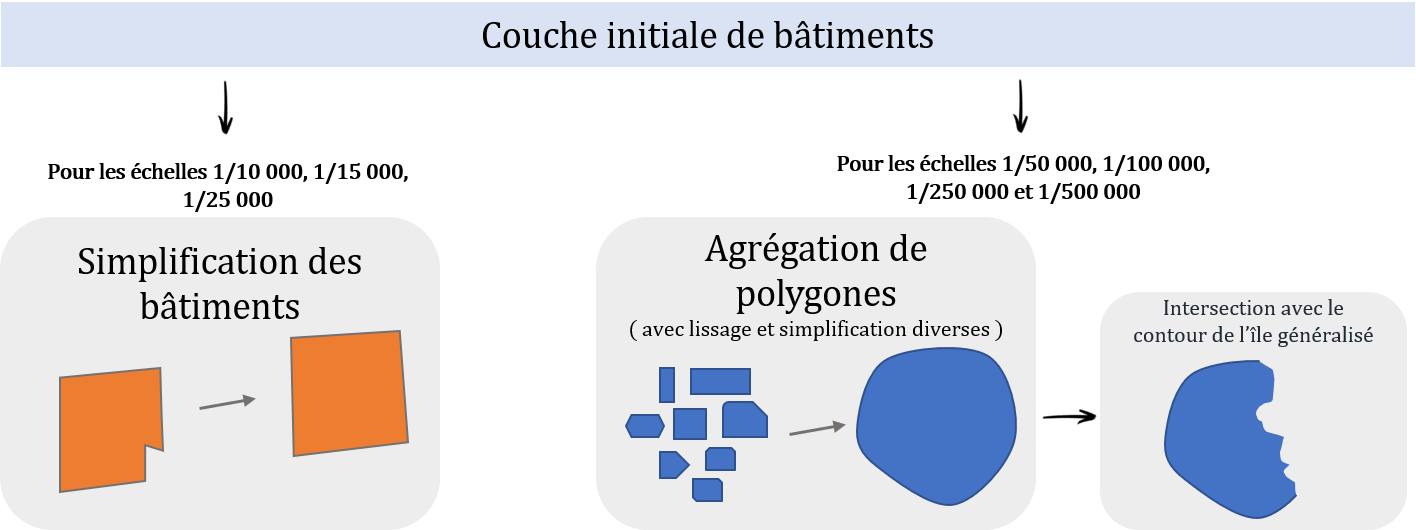
\includegraphics[width=\linewidth]{images/chap1/batiment_mb.png}
\caption{Explication schématique des traitements réalisés sur la couche EDI\_BATI}
\label{bati_mb}
\end{figure}

Les choix adoptés sont illustrés sur la figure \ref{bati_mb}. Le traitement \textbf{ Simplifier des bâtiments} est employé jusqu'à l'échelle 1/25000. C'est un traitement réalisé en dérivation ce qui signifie que le résultat pour chacune des échelles supérieures ou égales au 1/25 000 provient de la couche initiale calibrée pour le 1/5000. Il faut noter que l'outil \textit{"Simplifier les bâtiments"} d'ArcGIS propose d'éliminer les entités dont la superficie serait inférieure à une certaine valeur à définir. Cette option a été mise à profit pour supprimer les petits cabanons dans un premier temps puis les très petits bâtiments à des échelles inférieures. Sur la figure \ref{resultat_bati} (Carte A), on observe ces modifications de la géométrie ainsi que les suppressions de petits bâtiments. Tous les paramètres numériques des algorithmes font partie des métadonnées et se retrouvent dans l'annexe xx.

Pour les échelles inférieures ( du 1/500 000 au 1/50 000), la méthode est différente puisqu'elle s'appuie sur le traitement : \textbf{"Agréger les polygones"}. Il est non seulement possible de supprimer des entités trop petites mais aussi de gérer la taille des trous polygonaux. Comme l'illustre la figure  \ref{resultat_bati}, les trous polygonaux peuvent être pertinents au 1/50 000 (Carte B) mais le sont moins au 1/500 000 (Carte C).
dans cette gamme d'échelle, les traitements se font en série et par ordre d'échelle décroissante c'est à dire que la couche produite pour le 1/50 000 est à l'origine de celle produite pour le 1/100 000 et ainsi de suite. Pour assurer la cohérence de la cartographie et éviter que des agrégations de polygones ne viennent empiéter sur les lagons, un traitement supplémentaire ( cf model builder de l'annexe xx ) effectue l'intersection avec la la couche du contour de l'île adaptée. En effet, celle-ci étant aussi généralisée, l'intersection pour une échelle donnée se fait avec les entités adaptées à l'échelle.


\begin{figure}[ht]
\centering
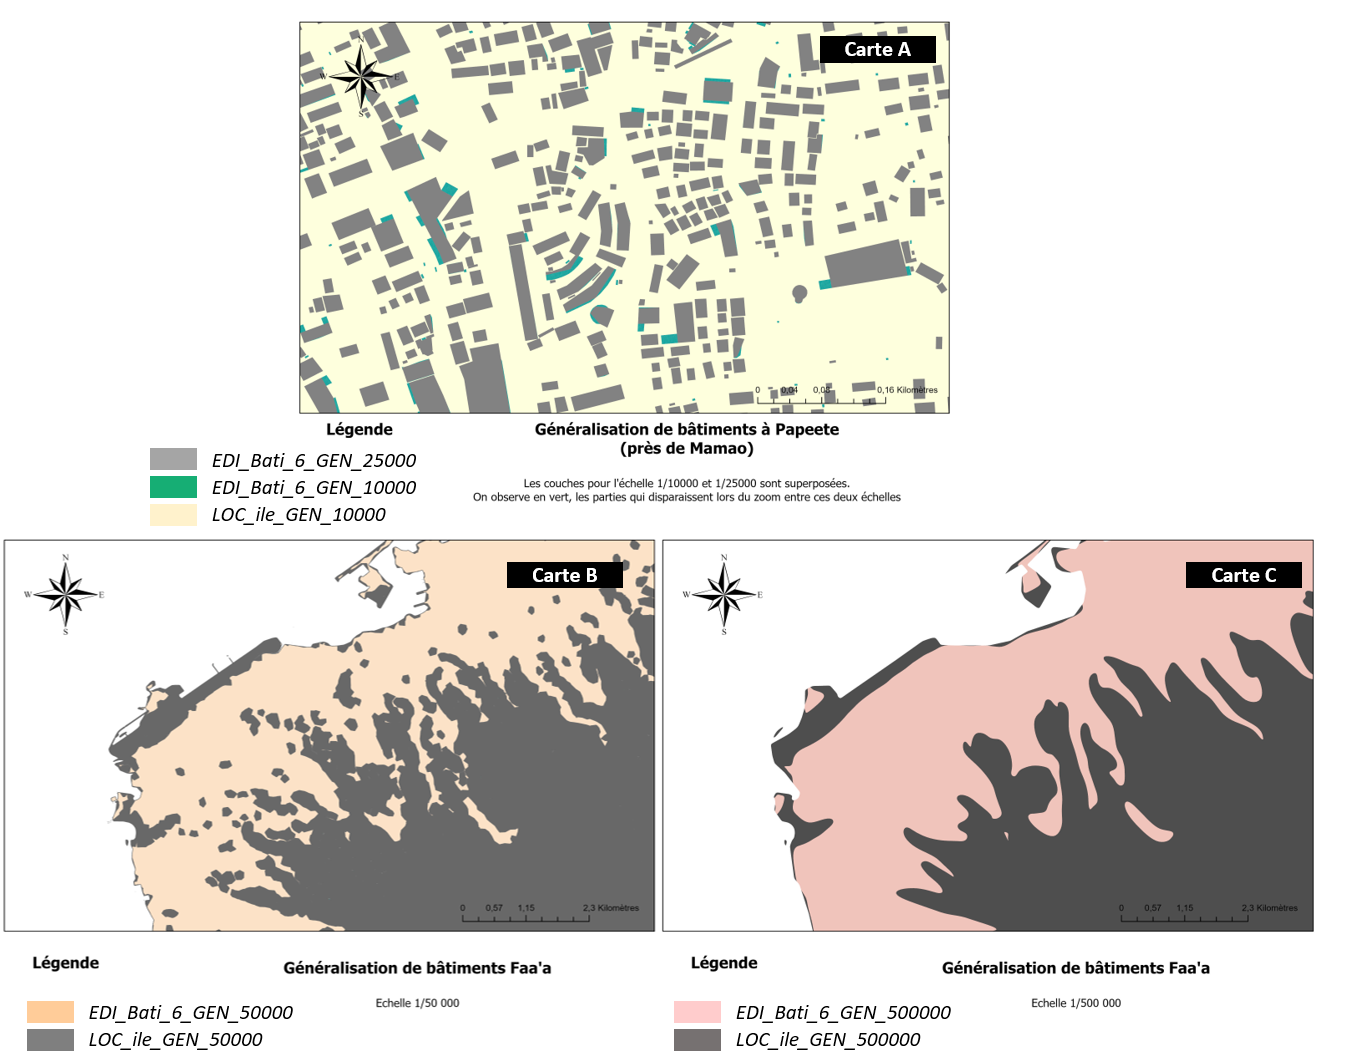
\includegraphics[width=\linewidth]{images/chap1/resultat_bati_bis.png}
\caption{Quelques résultats de généralisation sur la couche EDI\_BATI}
\label{resultat_bati}
\end{figure}

\begin{center}
    \textit{Quelles pistes d'amélioration ?}
\end{center}

Lors de la généralisation aux grandes échelles, il est parfois possible que des bâtiments se superposent. Les traitements sur ArcGIS permettent de signaler des conflits spatiaux avec un champ dédié. Cependant, le travail de gestion des conflits spatiaux n'a pas été fait car ces derniers étaient mineures. En effet les paramètres de simplification choisies restent relativement faibles et ne déforment pas suffisamment les bâtiments pour qu'un grand nombre d'entre eux se superposent. De plus, la suppression des petits cabanons évite de nombreux conflits spatiaux.

\subsection{Les constructions surfaciques}
\begin{center}
    \footnotesize
    \textbf{EDI\_CONSTRUCTION\_S}
\end{center}

Les constructions surfaciques sont généralisées de manière similaire à celle des bâtiments à la différence qu'elles ne sont jamais regroupées. Lorsque le point de généralisation qui correspond à l'échelle 1/25 000 est passé, alors la simplication de la géométrie est plus prononcée et le tri se fait de manière à ne garder que les entités d'intérêt. Tous les paramètres numériques utilisés figurent en annexe XX. On notera par exemple le choix d'une superficie minimale de 7000 m² pour l'échelle 1/50 000 de manière à ne conserver que les terrains de foot et autres constructions plus grandes tout en supprimant les terrains plus petits et plus nombreux qui ne serait pas lisibles sur la carte à cette échelle.

\textsc{Remarque :}
La présence des constructions surfaciques de grande ampleur peut se discuter à l'échelle 1/250 000. Il dépend notamment du support de la carte. S'il peut être pertinent de les placer sur une carte papier, leur présence se discute pour un support web multi-échelle. 

\subsection{Les limites administratives}

\begin{center}
    \footnotesize
    \textbf{LOC\_ile et LOC\_limite\_commune}
\end{center}

La couche LOC\_ile qui permet de connaître le contours des îles est composée d'entités surfaciques ( Une île représente un polygone ou un multi-polygone si elle est bordée de motus.)
La cellule topographie propose deux produits différents en ce qui concerne les communes.Le premier est une couche d'entités surfaciques correspondant aux communes tandis que le second est une couche d'entités linéaires faisant figurer les limites. Par ailleurs à Tahiti, le découpage administratif fait apparaître des regroupements de communes nommés "communes associées".\\

Les généralisations de ces deux couches, bien que leur géométrie soit différente, est similaire. Cela permet d'harmoniser les courbes de la carte. Pour ces deux couches, le traitement est le même pour toutes les échelles : il s'agit d'une simplication de ligne (ou polygone ) suivit d'un lissage. Les paramètres sélectionnés (voir annexe xx) sont choisis pour que le résultat soit approprié avec l'échelle.

En ce qui concerne les algorithmes, D-PK puis PAEK à décrire avec une figure

\subsection{Les lignes de relief}
\begin{center}
    \footnotesize
    \textbf{REL\_ligne\_relief}
\end{center}
L'annexe B décrit entre autres l'ensemble des catégories figurant dans la couche REL\_ligne\_relief. On observe de nombreux traits de reliefs. Certains sont à éliminer dès les premières échelles en dessous du 1/5000. C'est le cas notamment des éléments qui font partie de la catégorie \textit{Lignes caractéristiques}. 
{\color{magenta} NON REDIGE : Possible remarque sur les falaises et leur symbologie}

En ce qui concerne les courbes de niveau, la mise en évidence des courbes maîtresses et l'équidistance de celles-ci ne change pas jusqu'au 1/ 25 000 où le besoin de précision est extrêmement important. Il est à noter comme précisé dans la partie 2.1.2, que la carte au 1/25 000 est une carte topographique dont l'utilité comme c'est le cas en métropole peut être celle de la randonnée et de l'exploration. En effet, l'échelle est trop importante pour être utilisée pour le cadastre mais permet de couvrir avec précision une zone suffisamment grande pour visualiser quelques randonnées dans leur intégralité.

La généralisation pour les échelles plus petites nécessite des algorithmes complexes dans la mesure où les points côtés ne doivent pas être faussées et les lignes ne doivent pas s'intersecter. L'utilisation d'algorithmes de simplification de lignes comme ceux de Wang-Muller ou de Douglas-Peucker ne font pas l'affaire. La technique consiste à utiliser le généralisateur de Sherbend disponible sur le logiciel FME. 

Comme on peut le retrouver dans la documentation FME ainsi que dans les exemples \cite{sherbend}, le généralisateur de Sherbend ( SherbendGeneralizer) prend en entrée des lignes et des points et généralise avec un algorithme complexe et chronophage qui s'appuie sur celui de Douglas-Peucker de manière à ce que la généralisation ne change pas la position des points par rapport aux lignes ce qui s'avère intéressant pour maintenir la justesse de la carte.Les problèmes d'intersection de lignes sont aussi gérés par cet algorithme. Son utilisation à l'aide d'un script FME semble donc adpatée pour la généralisation des courbes de niveau au 1/50000\footnote{Aux échelles inférieures, les courbes de niveau n'ont pas été placées. Ce choix est inspiré de celui fait par l'IGN lors de la réalisation de la carte de TAHITI en 1988. Ce choix est discutable car le produit Plan IGN consultable sur le géoportail fait figurer des courbes de niveau. Par ailleurs, les courbes de niveau, qui permettent de mieux se répérer peuvent être un élément intéressant pour un portail web et d'une carte multi-échelle. La carte de l'IGN de 1988 compense cette absence de courbes de niveau par un relief très prononcé. (voir annexe \ref{sherbend})}.

\begin{figure}[ht]
\centering
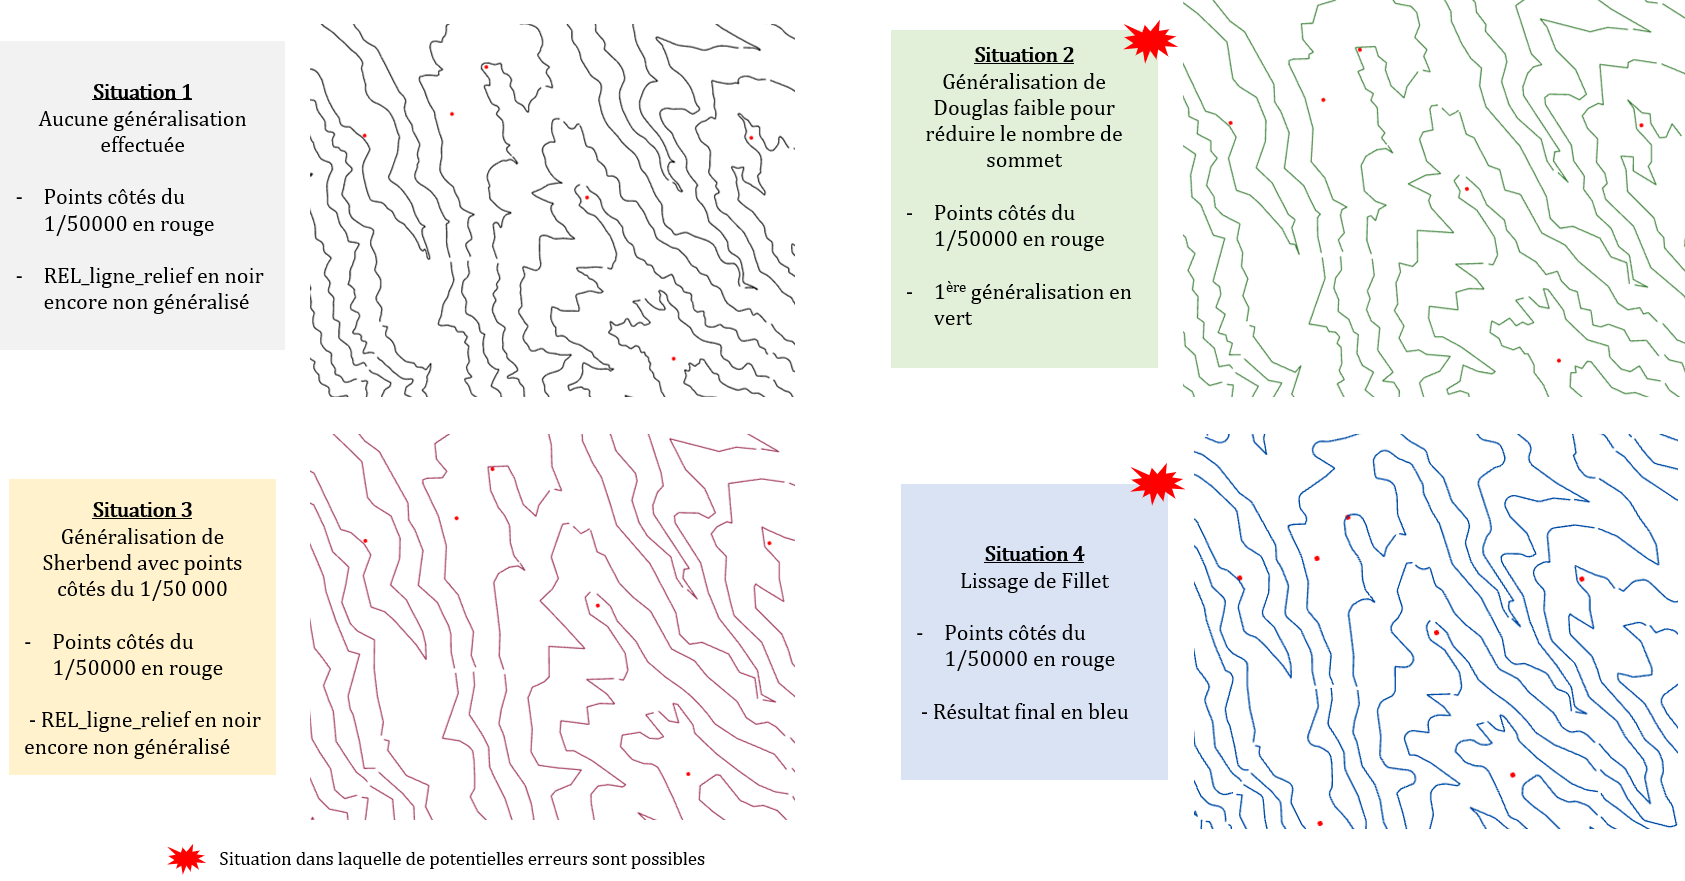
\includegraphics[width=\linewidth]{images/chap1/sherbend.png}
\caption{Quelques résultats de généralisation sur la couche EDI\_BATI}
\label{situation_sherbend}
\end{figure}
La figure \ref{situation_sherbend} décrit les étapes du processus de généralisation.
{\color{magenta} Cette solution n'est pas optimale et de potentielles erreurs sont possibles. }
Les données de départ sont les courbes de niveau non généralisée avec les points côtés  du 1/50000, c'est à dire ceux qui seront affichés sur la carte avec les courbes de niveau généralisée.
Un traitement préalable de sélection attributaire permet de ne garder que les courbes de niveau dites maîtresses (équidistantes de 100 m). Voici le descriptif des traitements ( illustrés par la figure \ref{situation_sherbend})
\begin{itemize}
\item Le premier traitement du script FME est une généralisation assez fine avec l'algorithme de Douglas-Peuker.  Ce traitement s'avère nécessaire pour permettre d'appliquer par la suite le traitement \textit{"SherbendGeneralizer"}. S'il n'est pas effectué , les temps de calculs seront beaucoup trop longs et cela d'autant plus si la généralisation ne s'applique sur toutes les courbes de niveau et non pas seulement comme c'est le cas ici sur les courbes maîtresses. Cependant, travailler sur des plus petites zones permet d'éviter cette étape. Il faut aussi noter que la généralisation est à priori assez fine et bien qu'il soit possible de fausser certains points avec cette étape, le risque reste faible avec les paramètres choisis ( paramètres détaillés dans l'annexe xx). A l'issu de ce traitement, le résultat est illustré par la Situation 2 de la figure \ref{situation_sherbend}
\item Le deuxième traitement est la généralisation de Sherbend à proprement parlé. Elle est paramétrée de manière à éviter les écueils qui peuvent survenir dans le cas d'une généralisation classique ( intersections de lignes et incohérence des courbes de niveau avec les points côtés). La simplification de ligne doit amener à la suppression des détails qui surchargeraient la carte au 1/50 000. A l'issu de ce traitement, le résultat est illustré par la Situation 2 de la figure \ref{situation_sherbend}
\item Enfin, le lissage est une dimension absente de l'algorithme précédent. Or l'absence de lissage est problématique pour le rendu cartographique. Cependant, comme c'était le cas dans l'étape 1, retoucher à la la géométrie des courbes de niveau signifie commettre potentiellement des erreurs sur les points côtés et sur la géométrie. Ainsi, pour limiter les potentielles erreurs, c'est un lissage de Fillet qui est choisi. Le principe de cet algorithme est d'arrondir les points anguleux d'une ligne avec comme paramètre un rayon (fixé à 0, la géométrie de la ligne est inchangée). Toute la problématique est donc de pouvoir produire un résultat suffisamment lissé sans générer d'erreurs. Enfin, la généralisation se tremine par la création d'un champ nommé \textit{"Classe\_1\_2" }qui établit une nouvelle classification des courbes obtenues. En effet, ces courbes, équidistantes de 100m, sont des courbes maitresse dans le classement initial. Un  nouveau classement établit des courbes maitresse tous les 500m.\\
\end{itemize}
\textsc{Remarques et pistes d'amélioration :}\\
Il est possible de ne pas commettre la première erreur en amont du généralisateur de Sherbend par un découpage plus détaillé des courbes de niveaux notamment sur Tahiti où leur nombre est important.

Pour ce qui est du lissage final (étape qui semble incontournable pour la lisibilité de la carte), il faudrait pouvoir mettre en place un système de contrôle de la géométrie et de la position des points côtés en fin d'algorithme de manière à prévenir des potentielles erreurs mais cette dimension n'a pas été abordée au cours de ce stage.



\subsection{Les tronçons hydrologiques et les surfaces d'eau}

La généralisation des cours d'eau est une étape délicate dans le processus de cartographie. En effet, à de petites échelles, une modification de la géométrie peut entraîner des conflits avec les autres couches, notamment les bâtiments. On ne saurait tolérer des inexactitudes géométriques allant jusqu'à la superposition de ces deux couches.Par ailleurs, une autre problématique correspond à la cohérence des surfaces d'eau avec les tronçons hydrologiques. Ainsi, les cartes réalisées au cours de ce projet font figurer des échelles 1/25 000 aux échelles 1/5000, la couche la plus détaillée de tronçons hydrographiques ainsi que la couche la plus détaillée de surface d'eau. La généralisation à effectuer entre ces échelles est simplement une sélection dans la table attributaire visant à éliminer certaines rigoles ou caniveaux trop insignifiant pour des échelles comme le 1/25 000. \footnote{Concernant ces couches, le travail de généralisation a donc été mineur jusqu'au 1/ 25 000. Jusqu'à cette échelle, la précision importante n'empêche pas la production d'une carte lisible, adaptée et cohérente. On notera  tout de même le cas de Raiatea (Île sous le Vent) où le nombre de tronçons hydrologiques répertoriés dans la base est très élevé ce qui surcharge énormément la carte au 1/25 000 alors que ça n'est pourtant pas le cas sur Tahiti}


\begin{center}
Comment généraliser ces deux couches à des échelles inférieures ?
\end{center}

\begin{center}
    \footnotesize
    \textbf{HYD\_troncon\_eau\_L}
\end{center}
Un possibilité pourrait être de considéré à partir du 1/50 000 uniquement les cours d'eau catégorisés pour cette échelle. Cependant, aucun champ de la base de donnée ne classe les cours d'eau. Une tentative a été faite en ne sélectionnant que les cours d'eau nommé car ces derniers sont jugés suffisamment important. Cependant cette méthode ne fonctionne pas car la base de donnée présente de nombreuses portions de cours d'eau non nommé. C'est donc une tout autre méthode qui doit être envisagée. Il s'agit d'une solution amenée à être provisoire en cas de restructuration future de la BDD.

Pour les petites échelles, les tracés hydrographiques se font à partir d'un MNT sur lequel des traitements hydrologiques ont été réalisés. Les documents de l'annexe xx détaillent ces traitements et les quantifient. dans cette annexe, un schéma simplifié décrit l'enchaînement des opérations.

{\color{magenta} NON-REDIGE Expliquer les opérations avec le schéma en annexe et les valeurs utilisées}
\begin{figure}[ht]
\centering
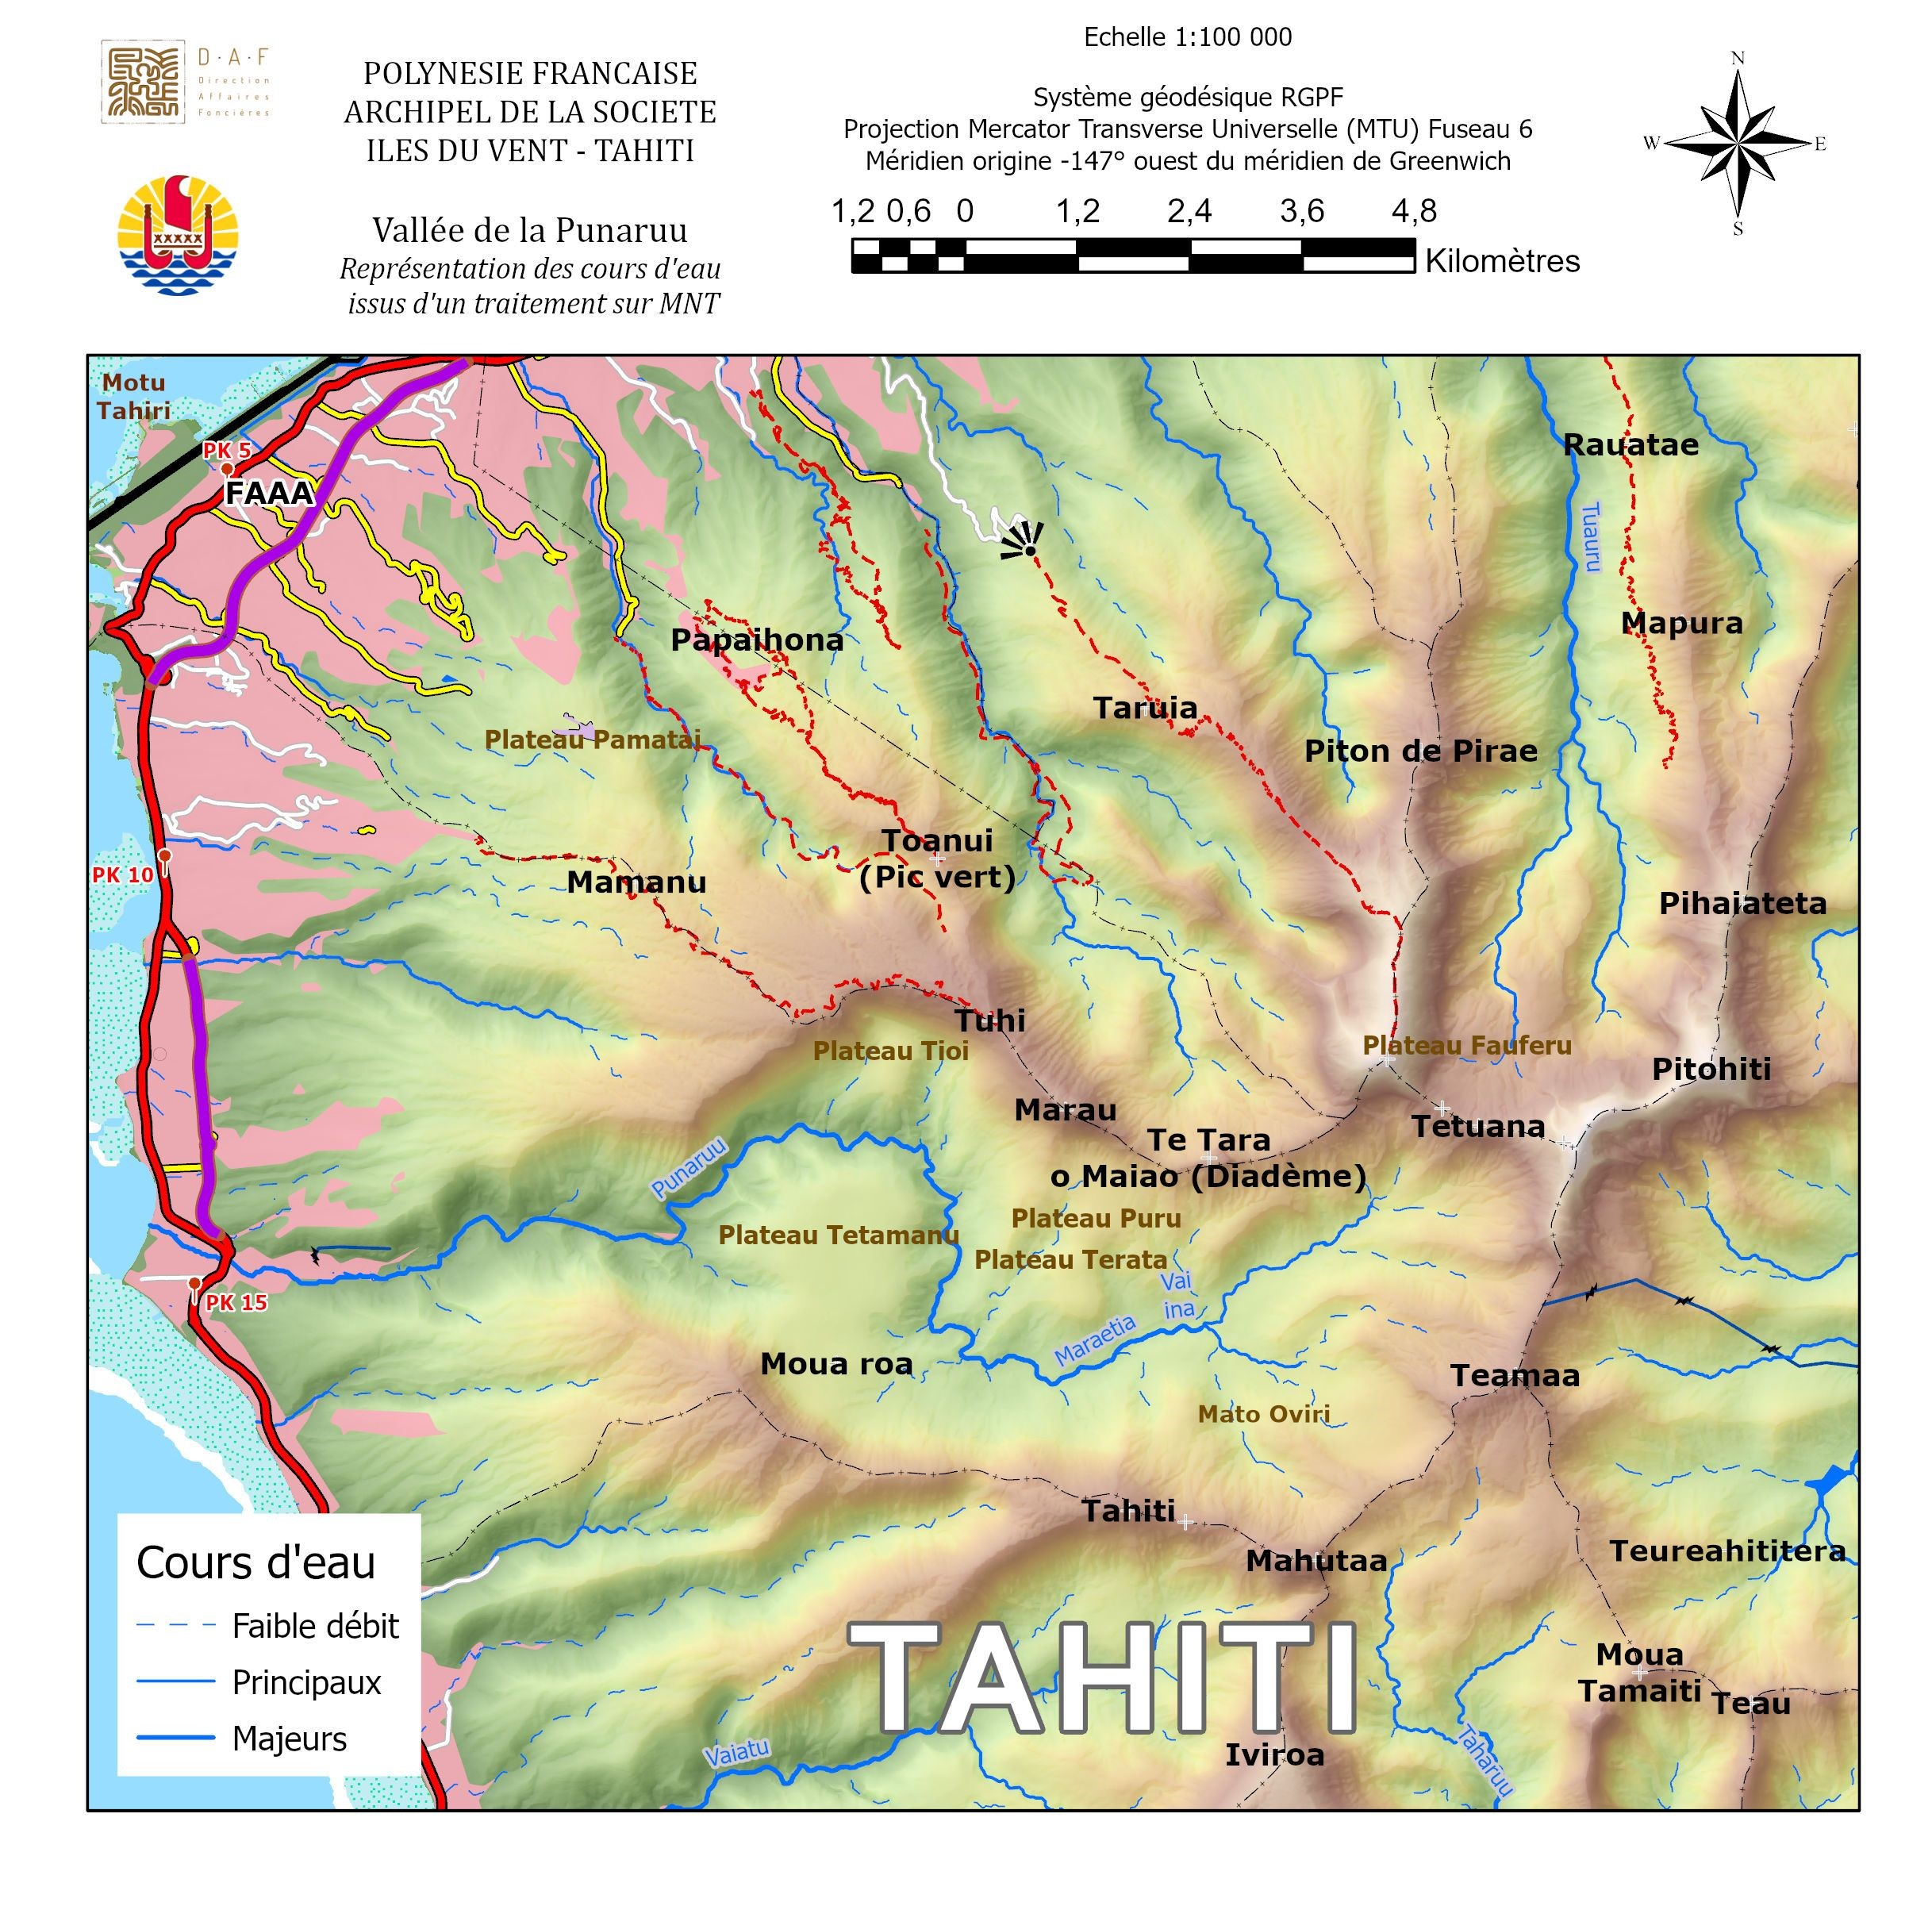
\includegraphics[scale=0.7]{images/chap1/carte_eau.jpg}
\caption{Représentation des cours d'eau issus du traitement sur MNT}
\label{carte_eau}
\end{figure}
Ce traitement à l'avantage de produire dans la table un champ GRID CODE contenant une valeur de 1 à 4 qui est un atout majeur pour la symbologie puisque ce champ qualifie l'importance du cours d'eau 

\begin{center}
    \footnotesize
    \textbf{HYD\_surface\_eau\_S}
\end{center}
Ce traitement complémentaire de simplification des polygones hydrologiques se base sur des simplifications de polygones ( avec élimination des entités de surface trop faible). Le modèle de ce traitement ainsi que les paramètres sont présents dans l'annexe xx

\section{Remarques et traitements secondaires}
\subsection{La voirie et sa catégorisation}
\begin{center}
    \footnotesize
    \textbf{VOI\_troncon\_route\_L, VOI\_limite\_route\_L et VOI\_mobilier\_route\_P }
\end{center}
La généralisation réalisée pour les couches qui concernent la voirie correspondant davantage à une restructuration du champ \textit{"classement" }pour avoir un nombre de catégories adapté à l'échelle. Parmi les opérations effectuées, on compte des suppressions d'entités, des groupements ainsi que des créations de champs. Ce travail est indissociable de la symbologie choisie qui fait l'objet de la partie suivante. Le travail s'est essentiellement porté sur la couche \textit{"VOI\_troncon\_route\_L"}. La couche \textit{"VOI\_limite\_route\_L"} devient quand à elle inutilisable pour des échelles trop petites tandis que la couche \textit{"VOI\_mobilier\_route\_P"} n'est utilisée que pour l'affichage des bornes. kilométriques\footnote{Il s'agit simplement d'une sélection attributaire étendue à une sélection sur le kilométrage de la borne (sélection tous les kilomètres ou tous les cinq kilomètres)}

{\color{magenta}PARTIELLEMENT REDIGE Le schéma XX ici ou en annexe en fonction de la place présente les catégories retenues à travers les différentes échelles.} On notera les difficultés pour mettre en évidence la route traversière de Tahiti. Une des propositions envisagées serait de créer dans la base de donnée un champ spécial pour les routes traversières présentes sur de nombreuses îles hautes en Polynésie.


\subsection{Remarques sur les couches ponctuelles}

Les couches d'entités ponctuelles nécessitent souvent une généralisation par sélection attributaire selon un champ \textit{"importance"} dédié. Les couches ponctuelles brièvement évoquées précédemment sont les couches de points côtés et de mobilier de route. Une couche ponctuelle qui a fait l'objet d'un travail de réflexion important est la couche \textbf{HYD\_point\_eau\_P}. On y retrouve notamment les sources, fontaines et cascades et la base de donnée ne fait pas encore figurer de champ permettant la généralisation. Différentes possibilités ont été envisagées pour généraliser la couche :
\begin{itemize}
\item Un traitement d'agrégation regroupant par exemple les cascades proches selon le centroïde. Cependant ce traitement entraîne des inexactitudes géométriques\footnote{qui peuvent néanmoins être tolérées}, mais aussi un problème dans la symbologie : faut-il mettre un symbole proportionnel au nombre de cascades regroupées ? comment négliger les cascades insignifiantes ?
\item La création d'un champ hauteur pour chacune des cascades répertoriées. La généralisation consisterait alors à trier en ne gardant que les plus grandes cascades lors du changement d'échelle. Cependant, une cascade n'est pas forcément signifiante uniquement par sa taille. Elle peut l'être aussi par son débit (souvent variable) ou sa position géographique. Toutes ces informations qui contribueraient à la construction d'une base de données extrêmement précises sont difficilement **renseignables** sur le nombre très conséquent de cascades que comporte la Polynésie.
\item la création d'un champ importance propre à chaque entité. Cette  solution semble la meilleur bien que contrairement à la précédente, elle n'apporte pas de précisions supplémentaires sur la donnée. Il s'agit cependant d'un vaste travail nécessitant potentiellement l'appel à des sociétés extérieures.\\
\end{itemize}

\textsc{Remarques diverses:}
\begin{itemize}
\item Les couches de Toponymes et de PAI sont des couches ponctuelles déjà généralisées. Elles servent pour l'étiquetage qui sera évoqué dans la partie suivante.
\item Certaines couchent ne sont pas généralisés (absence de modifications géométriques et de restructuration des champs pour la symbologie), soit parce qu'elles ne sont pas utilisées dans la cartographie (voir tableau de l'annexe xx) . Une des problématique non résolue de ce travail est la généralisation des couches d'occupation du sol notamment en zone urbaine. Pour rendre la carte lisible, les simplifications effectuées seront détaillées dans le chapitre suivant. 
\end{itemize}






\evenchapter{Production des cartes aux différentes échelles}

\textit{Une fois les couches généralisées, le travail suivant consiste à les assembler pour former les cartes. Il s'agit d'ajuster au mieux les couleurs et la superposition des couches, de choisir les ombrages adaptés et d'effectuer l'étiquetage en résolvant les conflits qui en découlent. La finalité est la production des cartes aux différentes échelles souhaitées ( cf Chap 2)}

\section{Création du fond de carte}
\textit{Les exemples présentés ci-dessous concernent les îles de Tahiti et de Moorea\footnote{ce qui correspond à la zone de travail initialement choisie}}

\subsection{Modèle Numérique de Terrain et Ombrage}

La section topographie de la DAF maintient différents modèles numériques de terrain de la Polynésie Française. Les plus récents sont des MNT Lidar datant de % et disponible uniquement sur la zone urbaine de Tahiti et le littoral (données bathymétriques ). 
Les ombrages réalisés dans le cadre de ce projet proviennent des MNT de 2013 pour Tahiti et Moorea ( précision du MNT: 25 m) En fonction de l'échelle, la finesse de l'ombrage doit être ajustée et pour cela, un ré-échantillonnage est nécessaire. Ainsi, à de petites échelles, un ré-échantillonage cubique 

\subsection{Occupation du sol sur les îles}

L'occupation du sol est gérée par une couche principale \textit{"SOL\_OCCUPATION\_S"} auxquels viennent s'ajouter des couches sur les limites végétales \textit{"SOL\_LIMITE\_VEGETALE"} et les arbres caractéristiques \textit{"SOL\_ARBRE\_CARACTERISTIQUE"}.  Organisée en catégories et sous-catégories, cette couche principale permet de représenter à l'occupation du sol en trois catégories ( végétation haute , basse naturelle, et plage) ainsi qu'en sous-catégories détaillées concernant les espaces agricoles, marécages / marais et mangroves. Aux grandes échelles riches en détailles, les catégories sont représentées en vastes zones de couleur tandis que les sous-catégories font l'objet d'un remplissage par pictogrammes ( par exemple des palmiers espacés pour représenter une cocoteraie). Pour l'échelle 1/50 000, comme on peut le voir sur la figure \ref{ocs}, cette double symbologie n'a plus été faite. On notera le traitement particulier pour l'échelle 1/25 000. Les bâtiments n'étant pas agrégés, la double symbologie s'avère lourde en zone urbaine.  Cependant, elle est toujours pertinente dans les zones moins habitées ou par exemple les zones de culture. C'est pourquoi, les zones urbaines au 1/25000 sont représentées sur un fond blanc issu de l'agrégation des bâtiments initialement calibrée pour le 1/250 000. De même,les couches annexes concernant les arbres caractéristiques et les limites végétales n'apparaissent plus car elles surchargeraient le fond de carte. Enfin, lors du passage de l'échelle 1/50 000 à l'échelle 1/100 000, celle-ci disparaît pour laisser place à un dégradé de couleur approprié à l'affichage du relief montagneux ou à un fond uni.\footnote{Ce rendu diffère de celui qui sera exporté sur le web en raison des problématiques d'ombrage qui seront évoqués dans le chapitre suivant.}

\begin{figure}[ht]
\centering
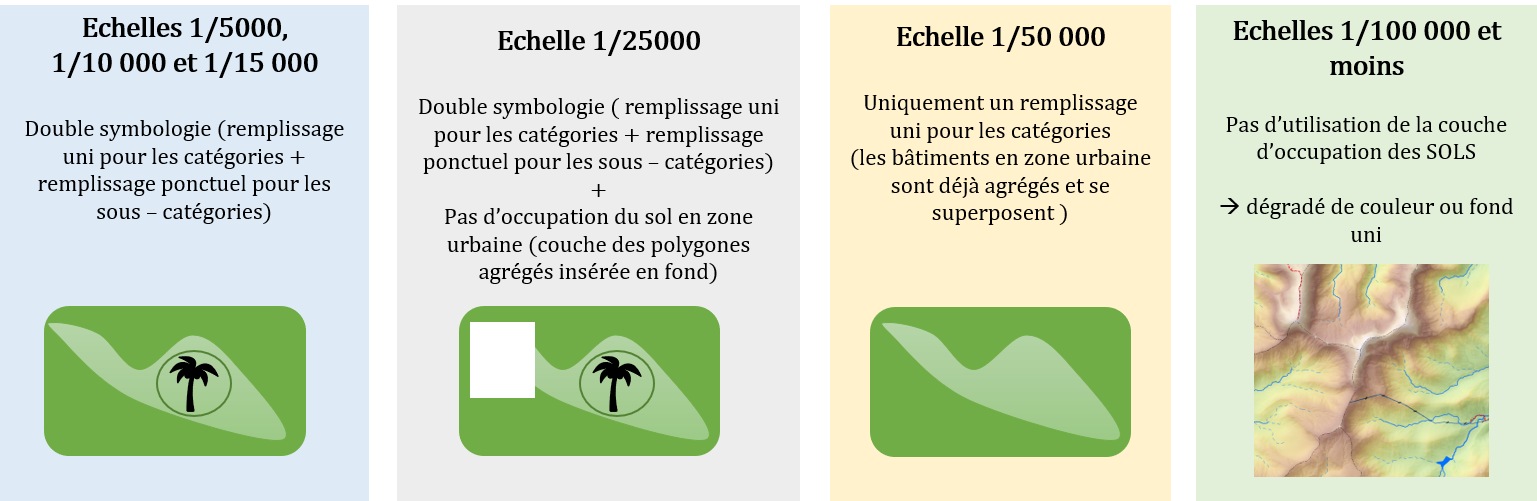
\includegraphics[width=\linewidth]{images/chap2/OCS.png}
\caption{Explication schématique de l'utilisation de la couche d'occupation des sols}
\label{ocs}
\end{figure}

\subsection{Cas des zones récifales lagonaires}

La cartographie des îles de la Polynésie est indissociable de la cartographie des récifs qui représentent des éléments incourtanables du relief. La section Topographie maintient dans sa base de donnée une couche d'entités linéaires
\textit{"HYD\_limite\_eau"}. Les multilignes tracent le contour des pâtés de coraux et des récifs mais cette couche est difficilement utilisables car imprécises. Par ailleurs, ce n'est pas une couche surfacique et elle ne permet pas, même avec des transformations sur SIG de distinguer les teintes de couleur des récifs.
Les cartes papier utilisent d'autres produits appelés fond cyan raster qui corespondent à des orthophotos rectifiée\footnote{la bande bleue est symbolisée par une échelle de cyan} et qui ont l'avantage de donner une représentation précise des zones littorales. Si les fonds cyans sont pertinents pour des échelles allant du 1/50 000 au 1/5000, ils ne le sont plus pour des échelles plus petites. La solution de contournement est l'utilisation de données de télédétection issues de ....
Un travail important permettant de simplifier les très nombreuses catégories scientifiques et les regrouper a été effectué. Il s'est notamment appuyé sur  l'Atlas des récifs coralliens de Polynésie française publié par des chercheurs néo-calédoniens en 2005 \cite{Noumea_2005}.
Elles permettent de classer les récifs de manière plus ou moins précises permettant de faire ressortir les zones d'eau peu profonde (couleur turquoise) ainsi que les barrières de corail. Ainsi, la cartographie au 1/500 000 ne fait figurer que les barrières de corail.

Cependant, ces dalles raster présente un désavantage majeur. Un masque turquoise ( couleur \#96DDFF ) à 100m des côtes doit être superposé aux dalles raster de forme carrée pour harmoniser les îles. Cependant, les teintes de bleu des dalles ne sont pas les mêmes d'îles en îles et posent donc un problème dès que la cartographie ne se limite plus à une seule île. Ce problème n'a pas été résolu et demeure donc sur les cartes dites "papier". En ce qui concerne l'export web, les limitations concernant l'usage de raster ont conduit à des choix de cartographie différents exposés dans le dernier chapitre.



\section {Placement des étiquettes}

Une des difficultés inhérentes au placement des étiquettes est la lisibilité. Les étiquettes doivent être adaptées à l'échelle et du 1/500 000 au 1/15 000, il n'existe pas dans la BD de la DAF de groupe d'annotations générées. Ainsi les étiquettes doivent être construites à partir des couches de points d'activités et des couches de toponymes. Le travail de généralisation n'est pas à faire. En effet pour ces deux couches, un champ \textit{"importance"} indique déjà les éléments à sélectionner. Le coeur du travail réside donc dans le placement et le style de celles-ci.

\begin{figure}[ht]
\centering
\includegraphics[width=\linewidth]{images/chap2/etiquette.jpg}
\caption{Carte de Papeete (généralisée pour l'échelle 1/25 000) permettant de visualiser les étiquettes}
\label{25eti}
\end{figure}

Si les couches \textit{NOM\_PAI} et \textit{NOM\_TOPONYME} représentent une grande partie des étiquettes sur les cartes, l'étiquetage se fait également sur des couches d'entités destinées à l'affichage comme les bornes kilométriques, les cours d'eau, ou encore les courbes de niveau.

\begin{center}
    Quelles contraintes respecter ?
\end{center}

La principale est bien entendu la cohérence des étiquettes entre les échelles. C'est une condition sine qua non au repérage de l'utilisateur entre les différentes échelles. Le code couleur doit donc être cohérent, ainsi que la police et sa taille. On observe sur la figure \ref{25eti} le travail réalisé à l'échelle 1/25 000. Plus de résultats peuvent être consultés en annexe.
On notera que la position des étiquettes par rapport à l'ombrage influe beaucoup sur le rendu final. Le choix qui a été effectué, influencé par la nécessité d'avoir une grande lisibilité, est de placer les étiquettes au dessus de l'ombrage à l'exception de celles concernant les courbes de niveau, car l'effet obtenu semble augmenter la perception du relief.

\begin{center}
    \textit{Quelques remarques sur les améliorations possibles et les problèmes d'étiquetage :}
\end{center}

En terme de symbologie, certains pictogrammes ont vocation à être améliorés comme pour les cascades. Un travail intéressant mais long et fastidieux serait de répertorier un angle d'orientation dans un champ de la table permettant d'orienter les symboles comme c'est le cas pour les noms des passes par exemple. Ensuite, les symboles des bornes kilométriques n'est pas satisfaisant. Une bonne représentation serait d'utiliser la forme des bornes réelles (se référer à la photo dans le glossaire), en plaçant l'étiquettes directement sur le symbole et au bon endroit. C'est un travail particulièrement long et technique nécessitant une très bonne maîtrises des outils d'étiquetage d'ArcGIS. Enfin, parmi les défauts d'étiquetage qui persistent après les multiples versions de cartes en papier, figure l'étiquetage des quartiers à Papeete. Il se fait par un texte noir entouré d'un halo blanc. Cependant, au milieu des nombreux bâtiments de la capitale, affichés en noir sur fond blanc à cette échelle, le résultat est mitigé. Il pourrait peut-être être amélioré par des traitements spécifiques à la capitale polynésienne ou par un changement dans la couleur des bâtiments qui serait alors problématique pour le rendu partout ailleurs.



\section {Résultats aux différentes échelles}

Pour valider le travail et savoir quelles corrections apporter, des échantillons de cartes ont été imprimés au format A0 pour un retour de l'ensemble des géomètres et géomaticiens de la section topographie de la DAF. Leurs remarques ont permis de retravailler certains algorithmes de généralisation ou encore certaines symbologies, police d'écriture ou couleur de fond de carte. 

La figure \ref{25_eti} ci-dessous présente un échantillon de  la carte au 1/25000 tandis que la figure \ref{100} est un extrait de la carte au 1/100 000. Compte-tenu du nombre d'échelles (8 niveaux) , l'ensemble des résultats figurent en annexe. Ces résultats ne sont pas ceux qui seront affichés sur le web. En effet, la publication des données dans un portail web nécessite de nombreuses simplifications qui font l'objet de la partie suivante. Par ailleurs, le portail web tient compte d'éventuelles retouchent liées au support de lecture et à l'harmonisation entre les niveaux de zoom. 
Cependant, ces supports papiers étaient indispensables à la préparation des couches en vue de l'export web. Ils pourront aussi servir après d'éventuelles retouches à fournir des exemplaires papiers sur demande des clients.

\begin{figure}[!h]
\centering
\includegraphics[width=5cm]{images/chap2/etiquette.jpg}
\caption{Carte centrée sur le nord de Tahiti (généralisée pour l'échelle 1/100 000)}
\label{100}
\end{figure}

\section{Remarques et critiques sur les choix de cartographie}
{\color{magenta} NON REDIGE : Liste des choses qui ne vont toujours pas sur les cartes, excepté les problèmes d'étiquetage évoqués plus haut}

\evenchapter{Création du portail cartographique}

\textit{Ce chapitre présente le travail de mise en ligne du portail cartographique sur la plateforme ArcGIS Online de la Direction des Affaires Foncières}

\section{Fond de plan multi-échelle}

\textit{Jusqu'à présent, chaque niveau d'échelle était représenté par une carte distincte. L'export sur ArcGIS Online a nécessité le regroupement des projets et la création d'un projet nommé "export\_web" entièrement dédié à l'export web.}

\subsection{ Préparation des projets pour l'export}

ArcGIS propose différentes façons d'exporter un projet, que ce soit en carte web ou en couche web.  \\

\textsc{Problèmes liés à l'export d'une couche web générale :}

Cette carte multi-échelle comprenant l'ensemble des données vectorielles et raster est impossible à exporter sur ArcGIS Online en raison du coup trop important (mesuré en crédits par ArcGIS)
Ce n'est pas tant la quantité de couches qui entraîne le dépassement du nombre de crédits alloués mais bien l'export de données raster.
Or dans la cartographie initiale, celles-ci sont multiples, qu'il s'agisse des fonds cyan pour la représentations des récifs ou encore des ombrages. Il a donc fallu trouver des alternatives.

Une des premières envisagée a été de convertir les couches raster en couches vectorielles. Pour le fond cyan, cela est passé par l'utilisation plus complète de la couche des récifs classés par télédétection. En groupant les catégories selon la méthode présentée en annexe xx du rapport, il a été possible de distinguer les éléments essentiels des récifs. Le résultat est bien entendu moins satisfaisant qu'avec les fonds cyans. \footnote{des problèmes de classification se sont posés et sont évoqués en annexe xx.}

En ce qui concerne l'ombrage, la possibilité d'un ombrage vectoriel a été envisagé puis abandonnée car le résultat n'est pas satisfaisant. S'il est coûteux d'exporter une gamme d'ombrages différents pour toutes les îles de la Polynésie, l'export d'un seul ombrage de Tahiti et Moorea l'est beaucoup moins. Cependant, la carte multi-échelle initiale ne peut faire figurer la couche d'ombrage qu'une seule fois. Son organisation en groupes de couches par niveau de zoom est pertinente lorsque chaque niveau de zoom a un ombrage adapté mais ne l'est plus en cas de simple ombrage. 

\begin{center}
    Quelle organisation a été mise en place pour pallier ces difficultés ?
\end{center}

Chaque niveau de zoom comporte des couches situées au dessus de l'ombrage et d'autres en dessous (comme cela a été évoqué dans le chapitre précédente). La solution adoptée est donc une scission de la carte générale multi-échelle précédentes en deux cartes, l'une nommée \textbf{\textit{Habillage\_multi\_echelle}} comportant pour chaque échelle, uniquement les couches destinées à être au dessus de l'ombrage et l'autre nommée  \textbf{\textit{Fond\_multi\_echelle}} comprenant uniquement des couches sur lesquels l'ombrage vient se superposer.
Ces deux cartes ne comportent pas de données raster et sont exportées sur ArcGIS Online en tant que couches web du même nom.

En ce qui concerne l'ombrage, ce dernier doit donc être placé entre les deux couches web précédentes. En utilisant la couche Terrain d'Esri, il est possible de ne pas avoir à exporter de données raster coûteuses sur ArcGIS Online. Mais comme en témoigne la figure \ref{ombrage} du chapitre 1, l'ombrage d'Esri est imprécis sur les zones montagneuses (souvent couvertes de nuages) de Tahiti. Il est donc utilisé à de petites échelles ne nécessitant pas un besoin important de précision et est combiné à un ombrage précis exporté sur une zone restreinte (Tahiti et Moorea) et pour des gammes d'échelles limitées dans l'optique de ne pas utiliser trop de crédits.  Cette couche web nommée \textbf{\textit{Ombrage\_TAH\_MOO}} est provisoire et doit être étendue sur toutes les îles hautes de la Polynésie française pour un rendu optimal sur le portail final.


\subsection{Utilisation d'un flux web de type tuiles vectorielles}

Deux éléments principaux doivent donc être exportées en couche web : l'habillage et le fond de carte.
Lors de l'export, différents modes sont possibles:
\begin{itemize}
    \item en tant qu'entités web
    \item en tant que tuiles
    \item en tant que tuiles vectorielles d'entités web
    \item en tant que tuiles vectorielles
\end{itemize}

Compte-tenu la multiplicité des couches et de leur symbologie composant les cartes \textbf{\textit{Fond\_multi\_echelle}} et \textbf{\textit{Habillage\_multi\_echelle}}, le partage en tant qu'entités web et tuiles vectorielles d'entités web s'avère infaisable. L'analyse indique de nombreuses erreurs liées à la non prise en charge du type de couche par ArcGIS.
Il reste donc deux possiblités dont une est beaucoup trop coûteuse en crédits : l'export en tuiles. En effet, ces tuiles, qui ne sont pas des tuiles vectorielles mais bel et bien raster représente un stockage immense dépassant les teraoctect de données sur de grandes échelles notamment en raison de l'ampleur de la zone à cartographier (l'équivalent de la superficie de l'Europe sans la Russie).

L'export se fait de chaque carte en couches web se fait donc via le mode tuiles vectorielles. ce mode présente l'avantage de pouvoir faire des mises à jour du style directement sur arcGIS online via un outil spécialisé permettant de manipuler directement le fichier JSON du style de la couche. Il est possible par exemple de changer la couleur des chemins, des routes, etc ) mais la couche résultante 


NON TERMINE





\section{Valorisation du fond de plan au travail d'applications thématiques}

\subsection{Géoportail et site web de la section topo}
{\color{magenta} Présenter les produits créés, comment les utiliser et leur vocation future (développement des thématiques en fonction des besoins)}

\subsection{Portail des fiches géodésiques et de nivellement}


 Qu'il s'agisse de cartes thématiques ( touristiques, de randonnée, etc...), de nombreux éléments peuvent être ajoutés à la carte actuelle. Par ailleurs, selon le thème choisi, il est possible de modifier l'habillage pour l'alléger et ainsi mettre en évidence cette thématique.

La dernière partie de ce projet qui concerne la diffusion des fiches géodésiques et de nivellement. L'objectif est de réaliser une version du portail qui soit spécialement consacrée à la diffusion de ces fiches pour les géomètres sur le terrain.
Il s'agit sur le portail précédemment créé, d'ajouter une couches des points de repère et de proposer au clic, une fenêtre contextuelle avec quelques information essentielles de la fiche ainsi qu'une photo. Le travail se découpe en plusieurs parties : 
\begin{itemize}
    \item Export depuis ARCGIS pro de la bonne version de la couche des repères avec la table des mesures associée
    \item Création sur Arcgis Pro d'une vue avec les éléments à diffuser
    \item Configuration de la fenêtre contextuelle avec les illustrations et les informations
    \item Ajout de la carte thématique au portail en ligne
\end{itemize}

{\color{magenta} Détailler les 4 items avec figures illustratives - ici, un bout seulement}

La fenêtre contextuelle doit contenir un condensé des éléments essentiels au géomètre qui devra trouver la majorité des renseignements nécessaires à cette endroit et pourra le cas échéant, accéder à la fiche pdf pour trouver des informations complémentaires. L'export qui à été décrit dans la partie ... permettait d'associer à la couche de donnée des pièces jointes incluant la photo au format jpeg ainsi que la fiche au format pdf. La fenêtre contextuelle doit d'abord faire figurer cette photo. Pour cela, un champ URL\_image doit être créé dans les champs de la couche pour y insérer le lien vers l'image en question. C'est par ce biais que l'image pourra être afficher dans la fenêtre contextuelle. La démarche de création du champ suit l'article de Gaetan Lavenu sur Arcorama \cite{lavenu} 

Cependant, la création du champ URL\_image différe de celui qui est proposé dans l'article car la couche des repères possède plusieurs pièces jointes et seules celles au format "image/jpeg" sont affichées dans la fenêtre. Le code permet donc de récupérer les id des pièces jointes désirées en les triant sur leur format selon qu'il s'agit de fiche pdf ou d'images jpeg. Ce code est expliqué en Annexe D. 
{\color{magenta} Détailler l'explication dans l'annexe}
\textsc{Remarques:} Une fois validée, la mise à jour du champ sur ArcGIS Online est particulièrement longue en ligne et nécessite environ 15 minutes pour 4000 éléments.


\section{Limites d'utilisation du portail}

\subsection {Limitations}
{\color{magenta} Détailler les problèmes  comme 
- les récifs
- les étiquettes
- l'absence de légende ( à voir avec ce qui a été déjà dit avant )
l'étiquetage sur les archipels et les cartes à des échelles supérieurs au 1/500 000. N'a pas été le principal thème de travail et les informations sont suffisantes sans être assez fournies avec quelques défauts d'étiquetage.
- l'ombrage imprécis d'esri+ Difficultés liées à la maintenance du portail et à la mise à jour des données}

\subsection {Axes d'amélioration}
Après avoir énuméré les limitations, cette sous-partie propose des axes d'amélioration pour la diffusion et la mise à jour d'un tel portail. 
{\color{magenta} 

- ombrage : soit la daf donne ses ombrages à esri pour éviter l'export assez coûteux (comme c'est le cas d'autres pays voir tableau). Ou alors export des ombrages. Problème, le nombre important d'îles hautes et donc d'ombrage. Le coût en crédit
- l'ombrage + Difficultés liées à la maintenance du portail et à la mise à jour des données}



%-------------------------------------------------------------------------------
\newevenpage
\chapter*{Conclusion}
  \addcontentsline{toc}{part}{Conclusion}
  \vspace{1.5cm}
    Ce travail exploratoire de 12 semaines a permis la création d'un portail cartographique avec les données topographiques. sa réalisation est d'abord passée par une importante phase de généralisation cartographique. Chacune des couches de la base de donnée a été diagnostiquée de manière à proposer un traitement adapté à la visualisation sur une large gamme d'échelle. ces traitements documentés sont expérimentaux et le résultat peut être réajusté via la modification des paramètres des Algorithmes qui ont été réalisé via ModelBuilder ou FME. Ils permettent néanmoins d'aboutir à une gamme de cartes topographiques de la Polynésie Française avec pour chacune d'entre elles, un étiquetage et une symbologie adaptée. La diffusion sur le web via ArcGIS Online, qui a été l'objectif principal de ce stage a nécessité de multiples adaptations du travail précédemment. Il a été notamment question de grouper les couches à la fois par gamme d'échelle pour s'adapter au niveau de zoom, mais aussi par nature selon qu'elles se superposent ou non à l'ombrage. Les données exportées sur la plateforme arcGIS online peuvent faire office de fond de carte. Leur diffusion en tant que tuiles vectorielles et la structure assez complexe du fond de carte rend leur mise à jour difficile. ******** Par ailleurs,   Enfin, ce stage s'est terminé par la diffusion des fiches géodésiques et de nivellement. cette thématique a permis d'aborder les problématiques liées à la configuration des fenêtres contextuelles sur ArcGIS Online. L'ensemble des outils crées ont été regroupé dans un site web tant que les métadonnées des couches et des traitements ont été transmise de manière à pouvoir être modifiées et améliorées dans l'optique de pouvoir un jour le diffuser au grand publique.


%-------------------------------------------------------------------------------
% Insertion de la bibliographie
\newevenpage
%\printbibheading
\printbibliography[title={Bibliographie}]
\nocite{*}

\newevenpage
\listoffigures

\newevenpage
\listoftables
%----------------------------------------------------

\begin{appendices} 
\label{beginappendices}

%%%%%%%%%%%%%%%%%%%%%%%%%%%%%%%%%%%%%%%%%%%%%%%%%%%%%%%%%%%%%%%%%%%%%%%%%%
%%%%%%%%%%%%%%%%%%%%%   ANNEXE A  %%%%%%%%%%%%%%%%%%%%%%%%%%%%%%%%%%%%%%%%
%%%%%%%%%%%%%%%%%%%%%%%%%%%%%%%%%%%%%%%%%%%%%%%%%%%%%%%%%%%%%%%%%%%%%%%%%%


\annexe[Base de données de la Polynésie Française - Diagramme de classe]{ Architecture de la base de Données de la Polynésie Française \newline \textit{Diagramme de classes}}
\label{annexearchitecure}

La prise en main de la base de donnée nécessite de connaître l'ensemble des tables qui la compose ainsi que leurs attributs. Un diagramme fournit en début de stage, permet de bien visualiser l'architecture complète de la base. Ce diagramme précise l'ensemble des attributs et est indispensable pour préparer en amont la symbologie. Ce diagramme UML fait figurer l'ensemble des classes concernant la cartographie.\footnote{Dans ces diagrammes, chacune des classes est bien souvent la représentation schématique d'une couche dans un SIG. Ainsi le diagramme présente les attributs sur lesquels le travail dans un SIG pourra porter. Cependant, il existe des classes qui n'ayant pas de géométrie associée, se caractérisent simplement par des tables. C'est pourquoi le tableau en début d'annexe précise notamment ces informations.}





\begin{figure}[!h]
\centering
\subfigure{\label{fig:graphics:a}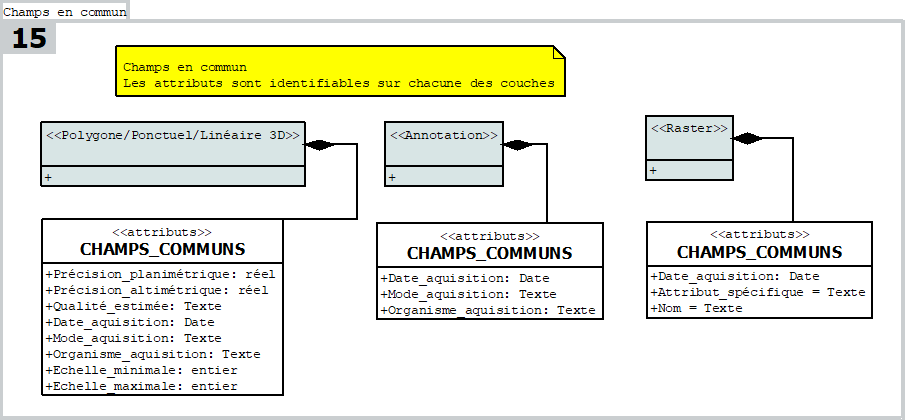
\includegraphics[width=\linewidth]{images/Architecture_BDD/CHAMP_COMMUN.png}}
\caption{Champs en commun pour tous les classes}%
\textit{On les retrouve sur toutes les couches + autre commentaire }
\label{fig:graphics}% label for figure
\end{figure}

\addtocounter{figure}{-1}
\begin{figure}
\addtocounter{figure}{1}
\centering
\subfigure{%
\label{fig:graphics:b}% label for subfigure
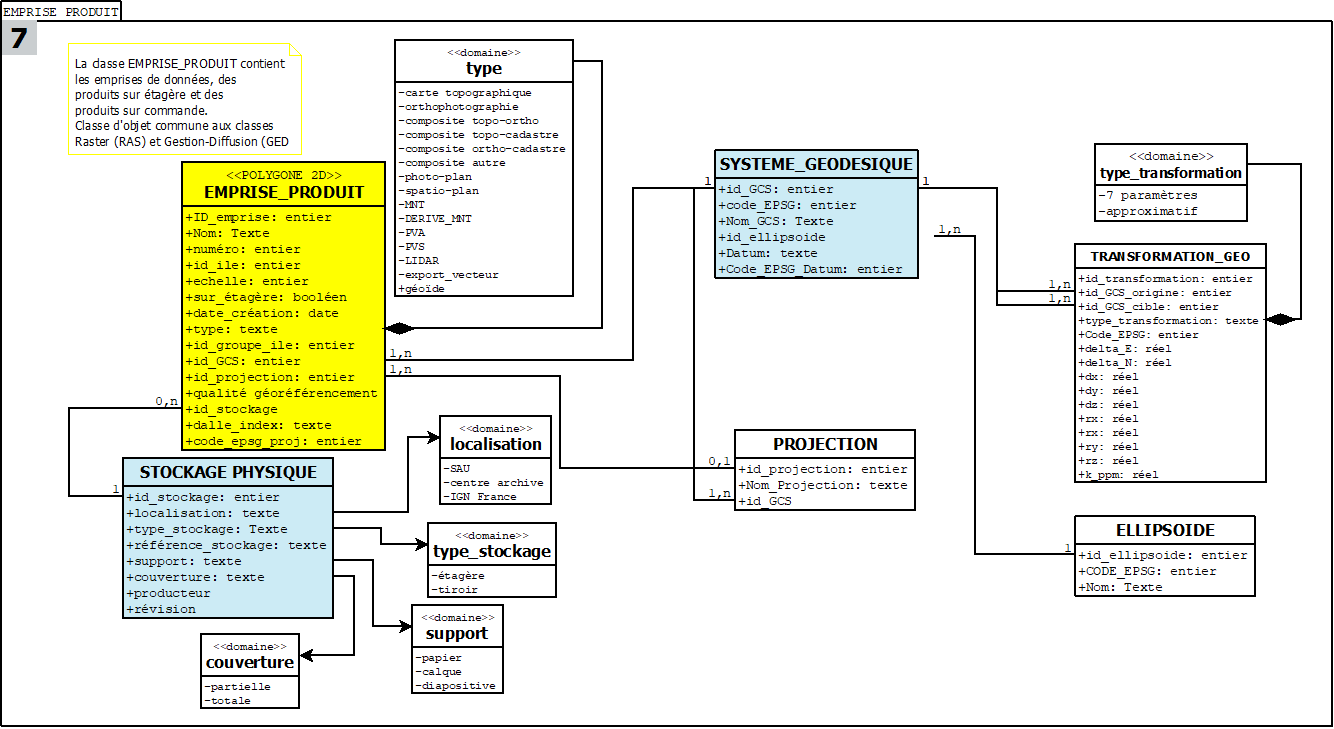
\includegraphics[width=\linewidth]{images/Architecture_BDD/EMPRISE_PRODUIT.png}}%
\caption{Diagramme des emprises des produits}%
\textit{Cette classe figure ici à titre informatif. Elle caractérise une couche qui n'est pas utilisée pour la cartographie et qui n'a pas vocation à être généralisée.}
\end{figure}

\addtocounter{figure}{-1}
\begin{figure}
\addtocounter{figure}{1}
\centering
\subfigure{%
\label{fig:graphics:b}% label for subfigure
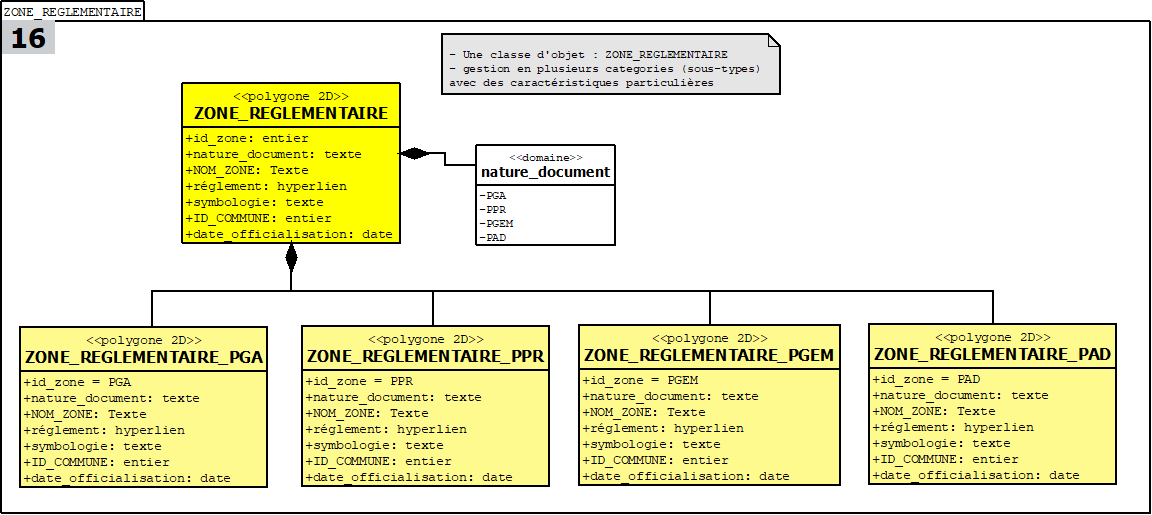
\includegraphics[width=\linewidth]{images/Architecture_BDD/EXT_ZONE_REGLEMENTAIRE.png}}%
\caption{Diagramme de la classe des zones réglementaires}%
\textit{Cette classe figure ici à titre informatif. Elle caractérise une couche qui n'est pas utilisée pour la cartographie et qui n'a pas vocation à être généralisée.}
\end{figure}

\addtocounter{figure}{-1}
\begin{sidewaysfigure}
\addtocounter{figure}{1}
\centering
\subfigure{%
\label{fig:graphics:b}% label for subfigure
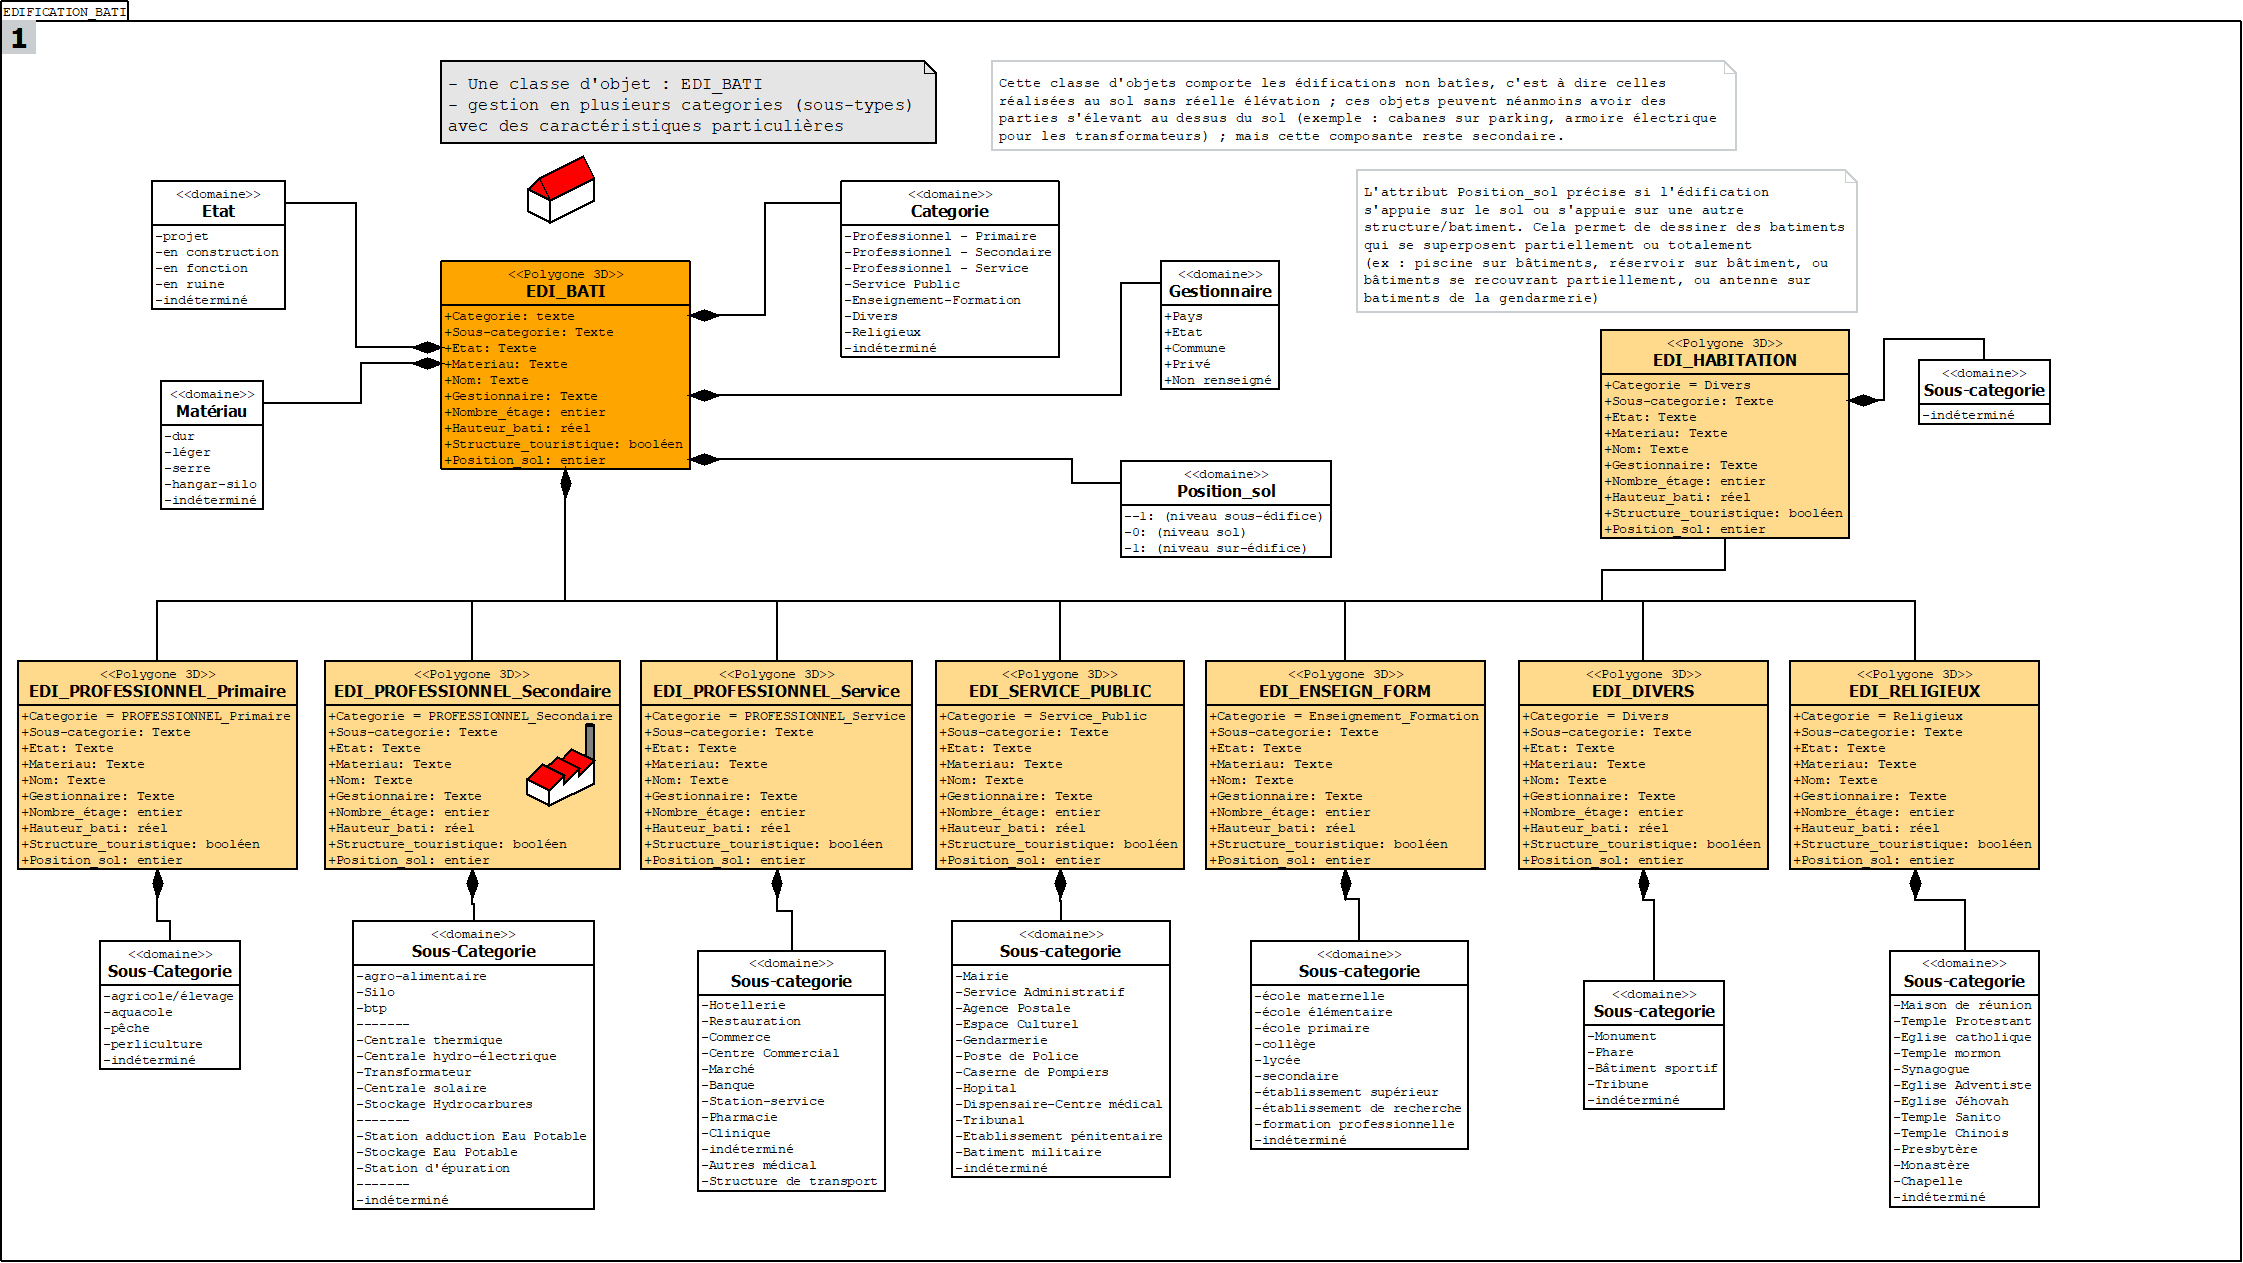
\includegraphics[width=\linewidth]{images/Architecture_BDD/EDI_BATI.png}}%
\caption{Diagramme de la classe des bâtiments}%
\end{sidewaysfigure}

\addtocounter{figure}{-1}
\begin{sidewaysfigure}
\addtocounter{figure}{1}
\centering
\subfigure{%
\label{fig:graphics:b}% label for subfigure
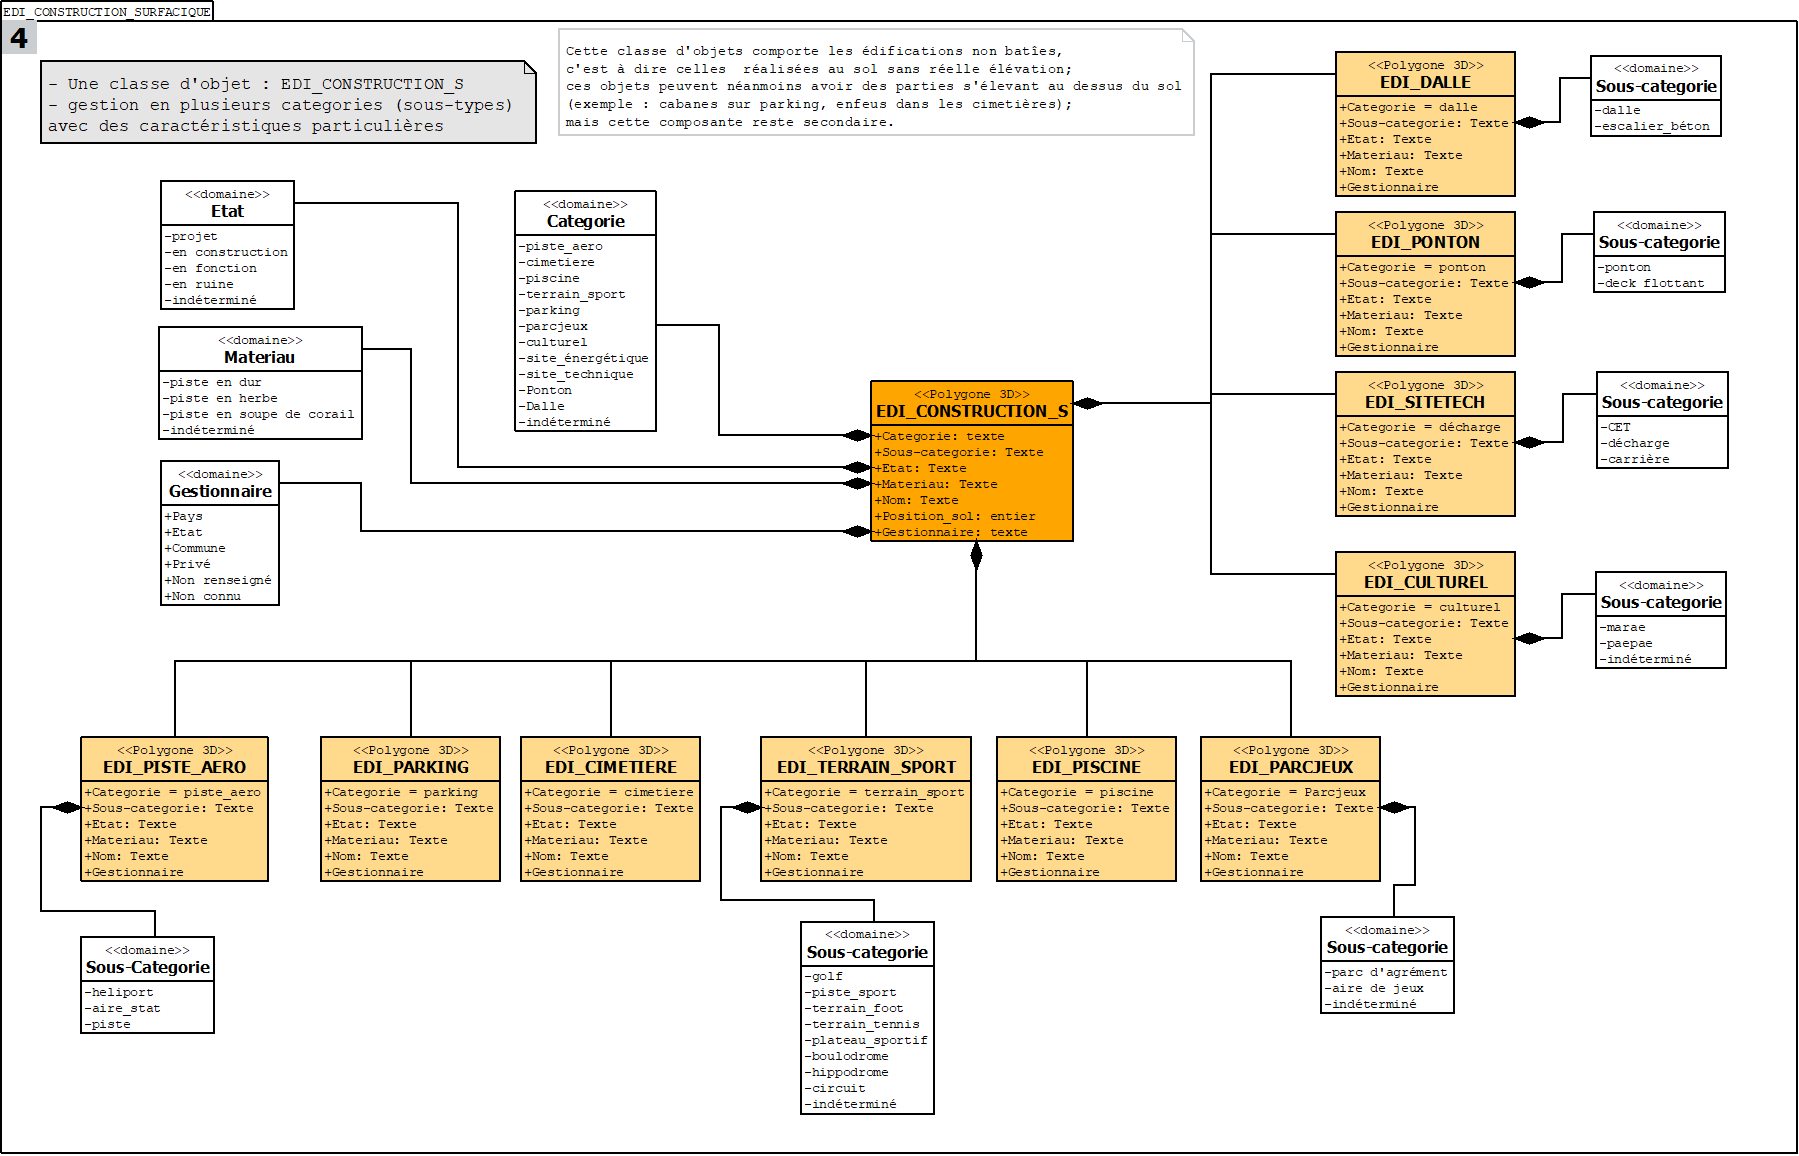
\includegraphics[width=\linewidth]{images/Architecture_BDD/EDI_CONSTRUCTION_S.png}}%
\caption{Diagramme de la classe des constructions surfaciques}%
\end{sidewaysfigure}

\addtocounter{figure}{-1}
\begin{figure}
\addtocounter{figure}{1}
\centering
\subfigure{%
\label{fig:graphics:b}% label for subfigure
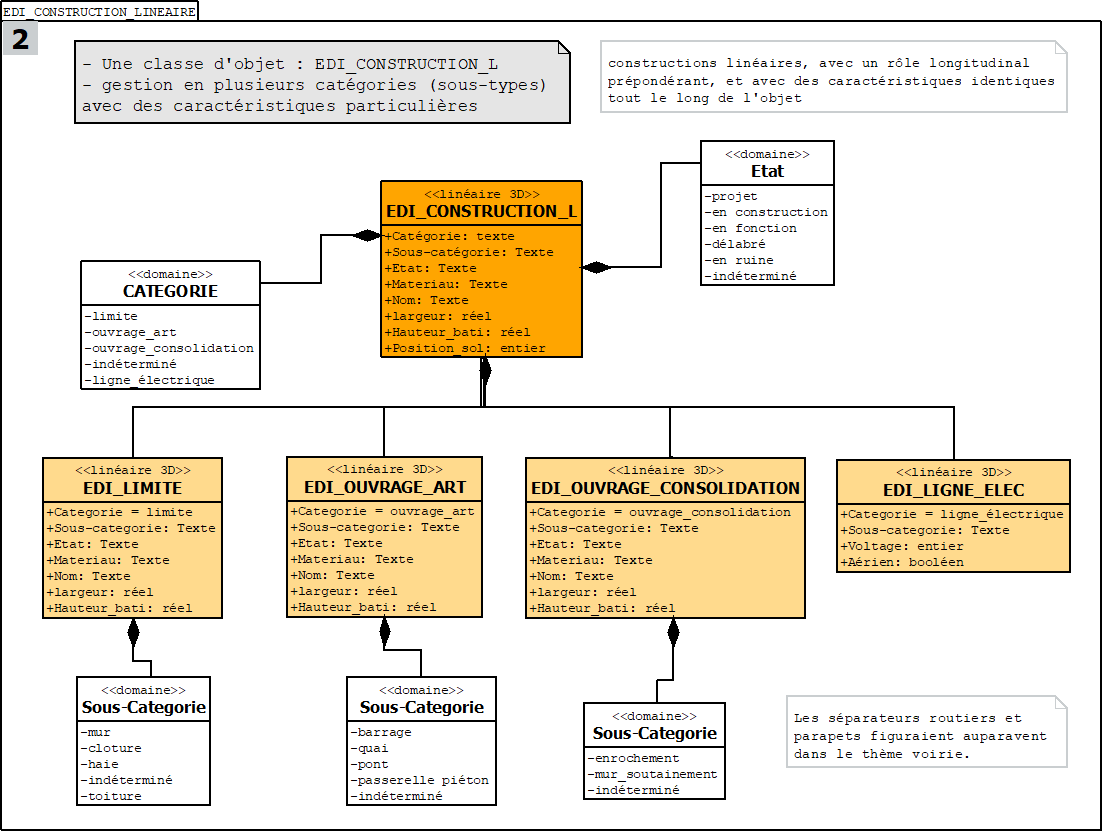
\includegraphics[width=\linewidth]{images/Architecture_BDD/EDI_CONSTRUCTION_L.png}}%
\caption{Diagramme de la classe des constructions linéaires}%
\end{figure}

\addtocounter{figure}{-1}
\begin{sidewaysfigure}
\addtocounter{figure}{1}
\centering
\subfigure{%
\label{fig:graphics:b}% label for subfigure
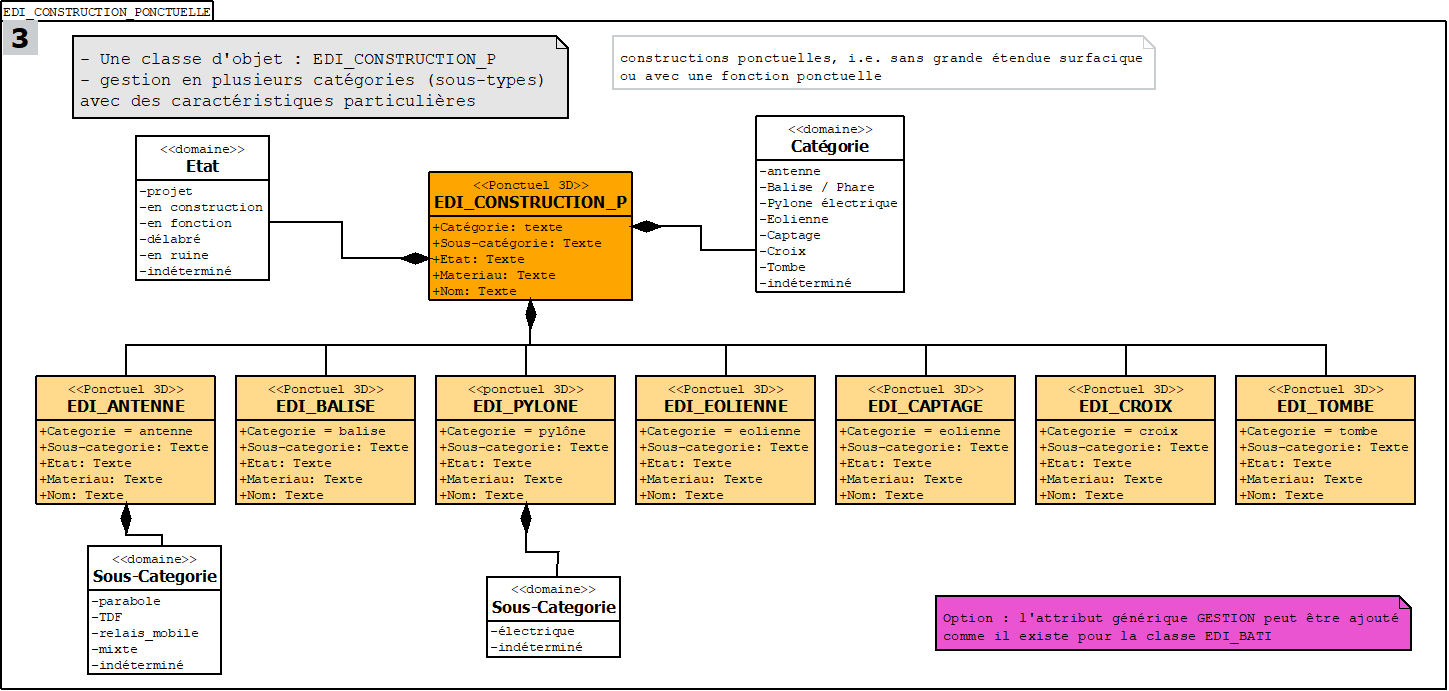
\includegraphics[width=\linewidth]{images/Architecture_BDD/EDI_CONSTRUCTION_P.png}}%
\caption{Diagramme de la classe des constructions ponctuelles}%
\end{sidewaysfigure}

\addtocounter{figure}{-1}
\begin{sidewaysfigure}
\addtocounter{figure}{1}
\centering
\subfigure{%
\label{fig:graphics:b}% label for subfigure
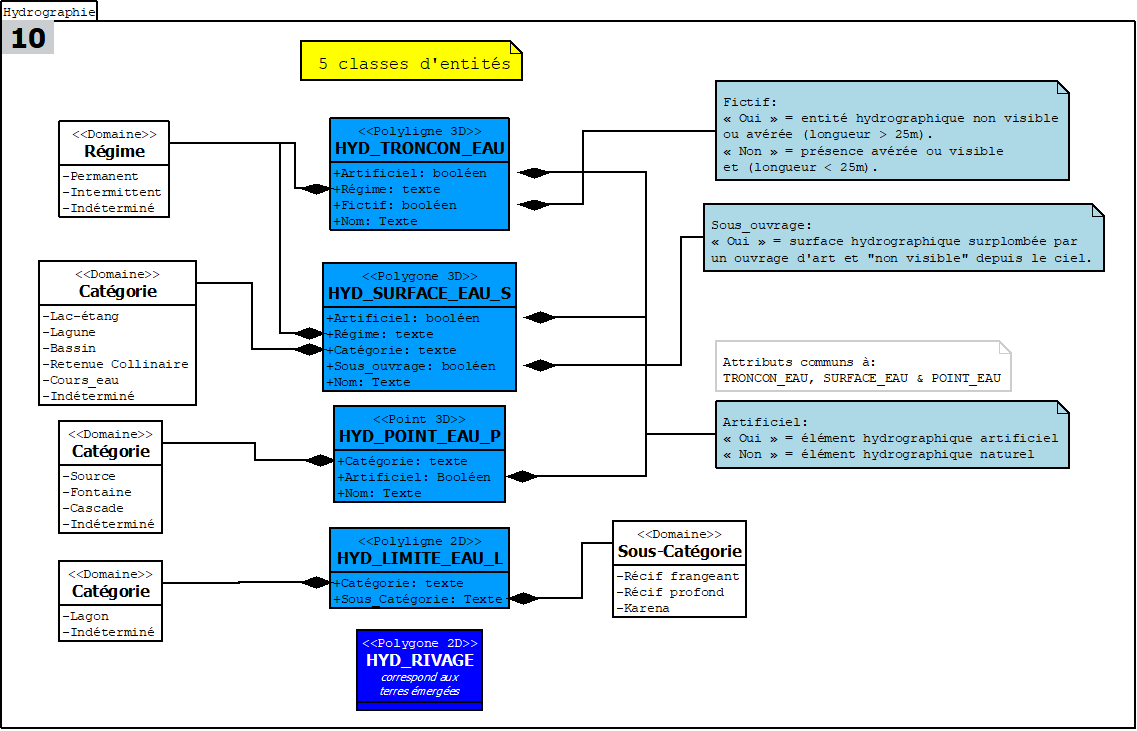
\includegraphics[width=\linewidth]{images/Architecture_BDD/HYD_HYDROGRAPHIE.png}}%
\caption{Diagramme des classes concernant la thématique hydrographie}
\end{sidewaysfigure}

\addtocounter{figure}{-1}
\begin{sidewaysfigure}
\addtocounter{figure}{1}
\centering
\subfigure{%
\label{fig:graphics:b}% label for subfigure
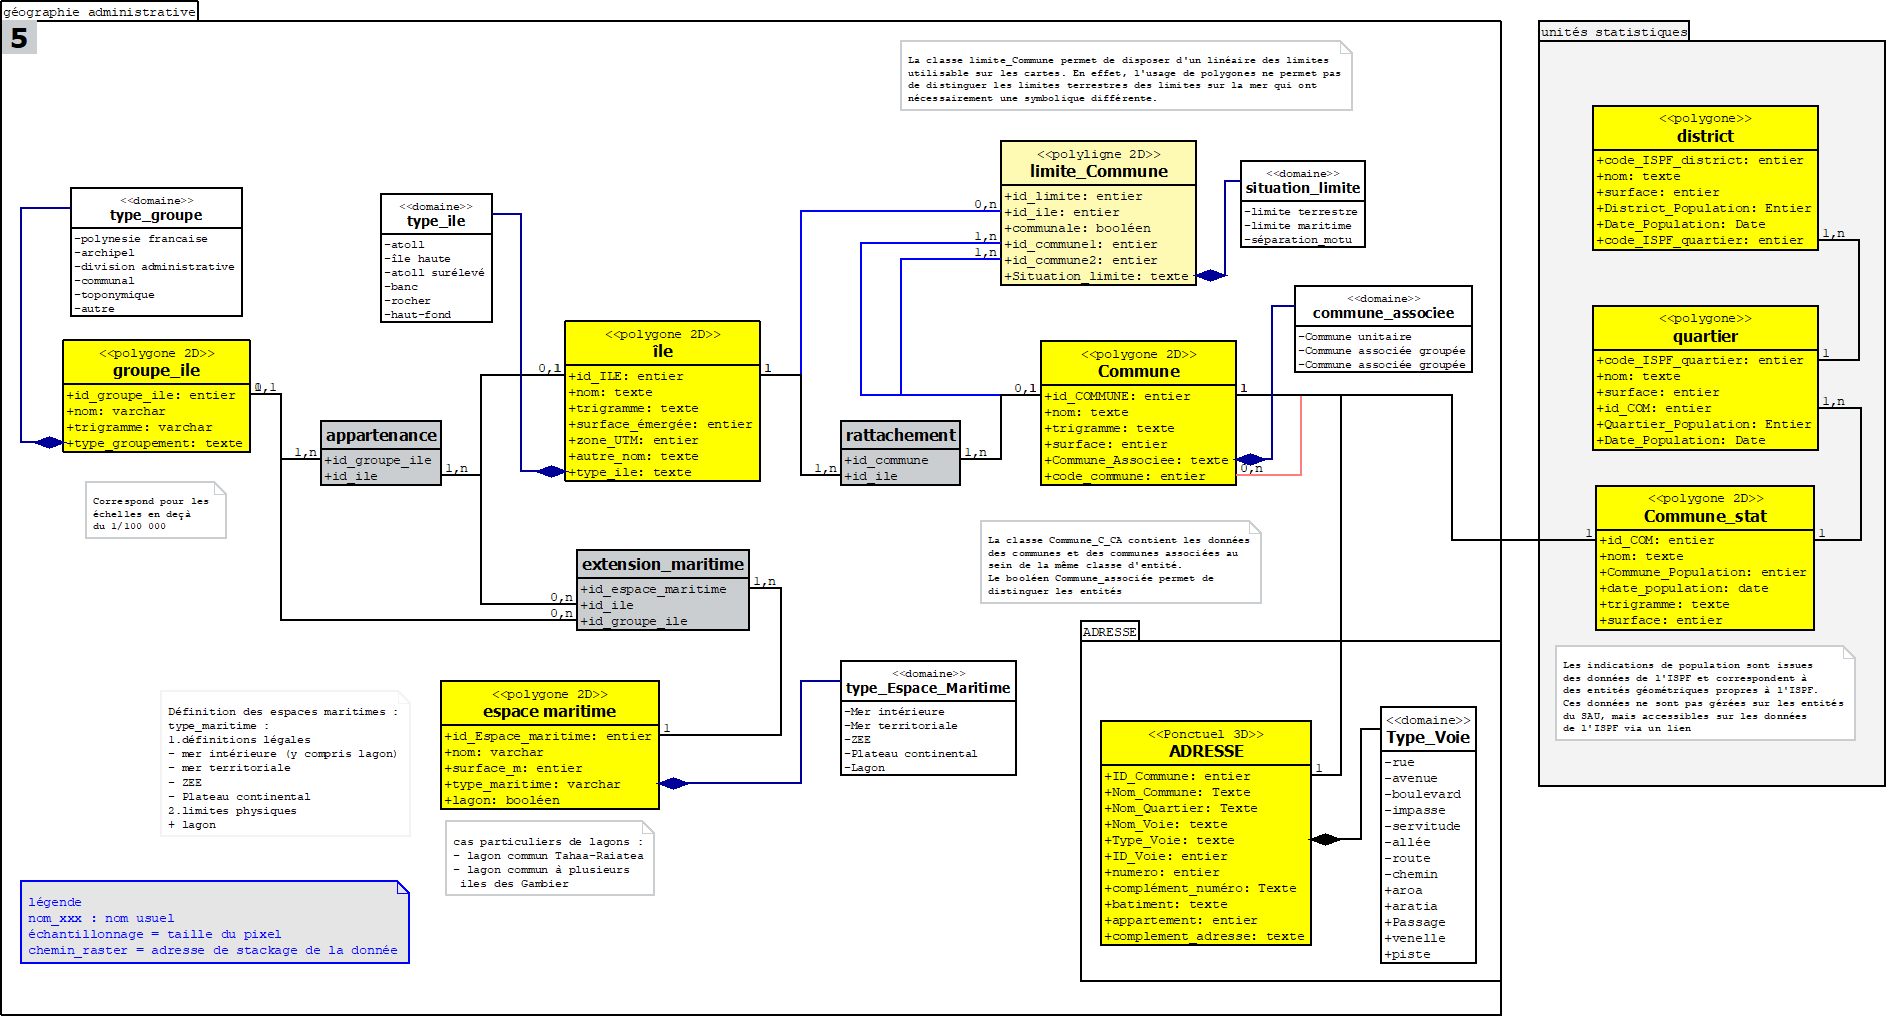
\includegraphics[width=\linewidth]{images/Architecture_BDD/LOC_LOCALISATION_ADMIN.png}}%
\caption{Diagramme des classes de la géographie administrative}%
\textit{Des classes d'unités statistiques figurent également et renseignent un peu plus les classes purement liées à la géographie et au contour des entités}
\end{sidewaysfigure}

\addtocounter{figure}{-1}
\begin{sidewaysfigure}
\addtocounter{figure}{1}
\centering
\subfigure{%
\label{fig:graphics:b}% label for subfigure
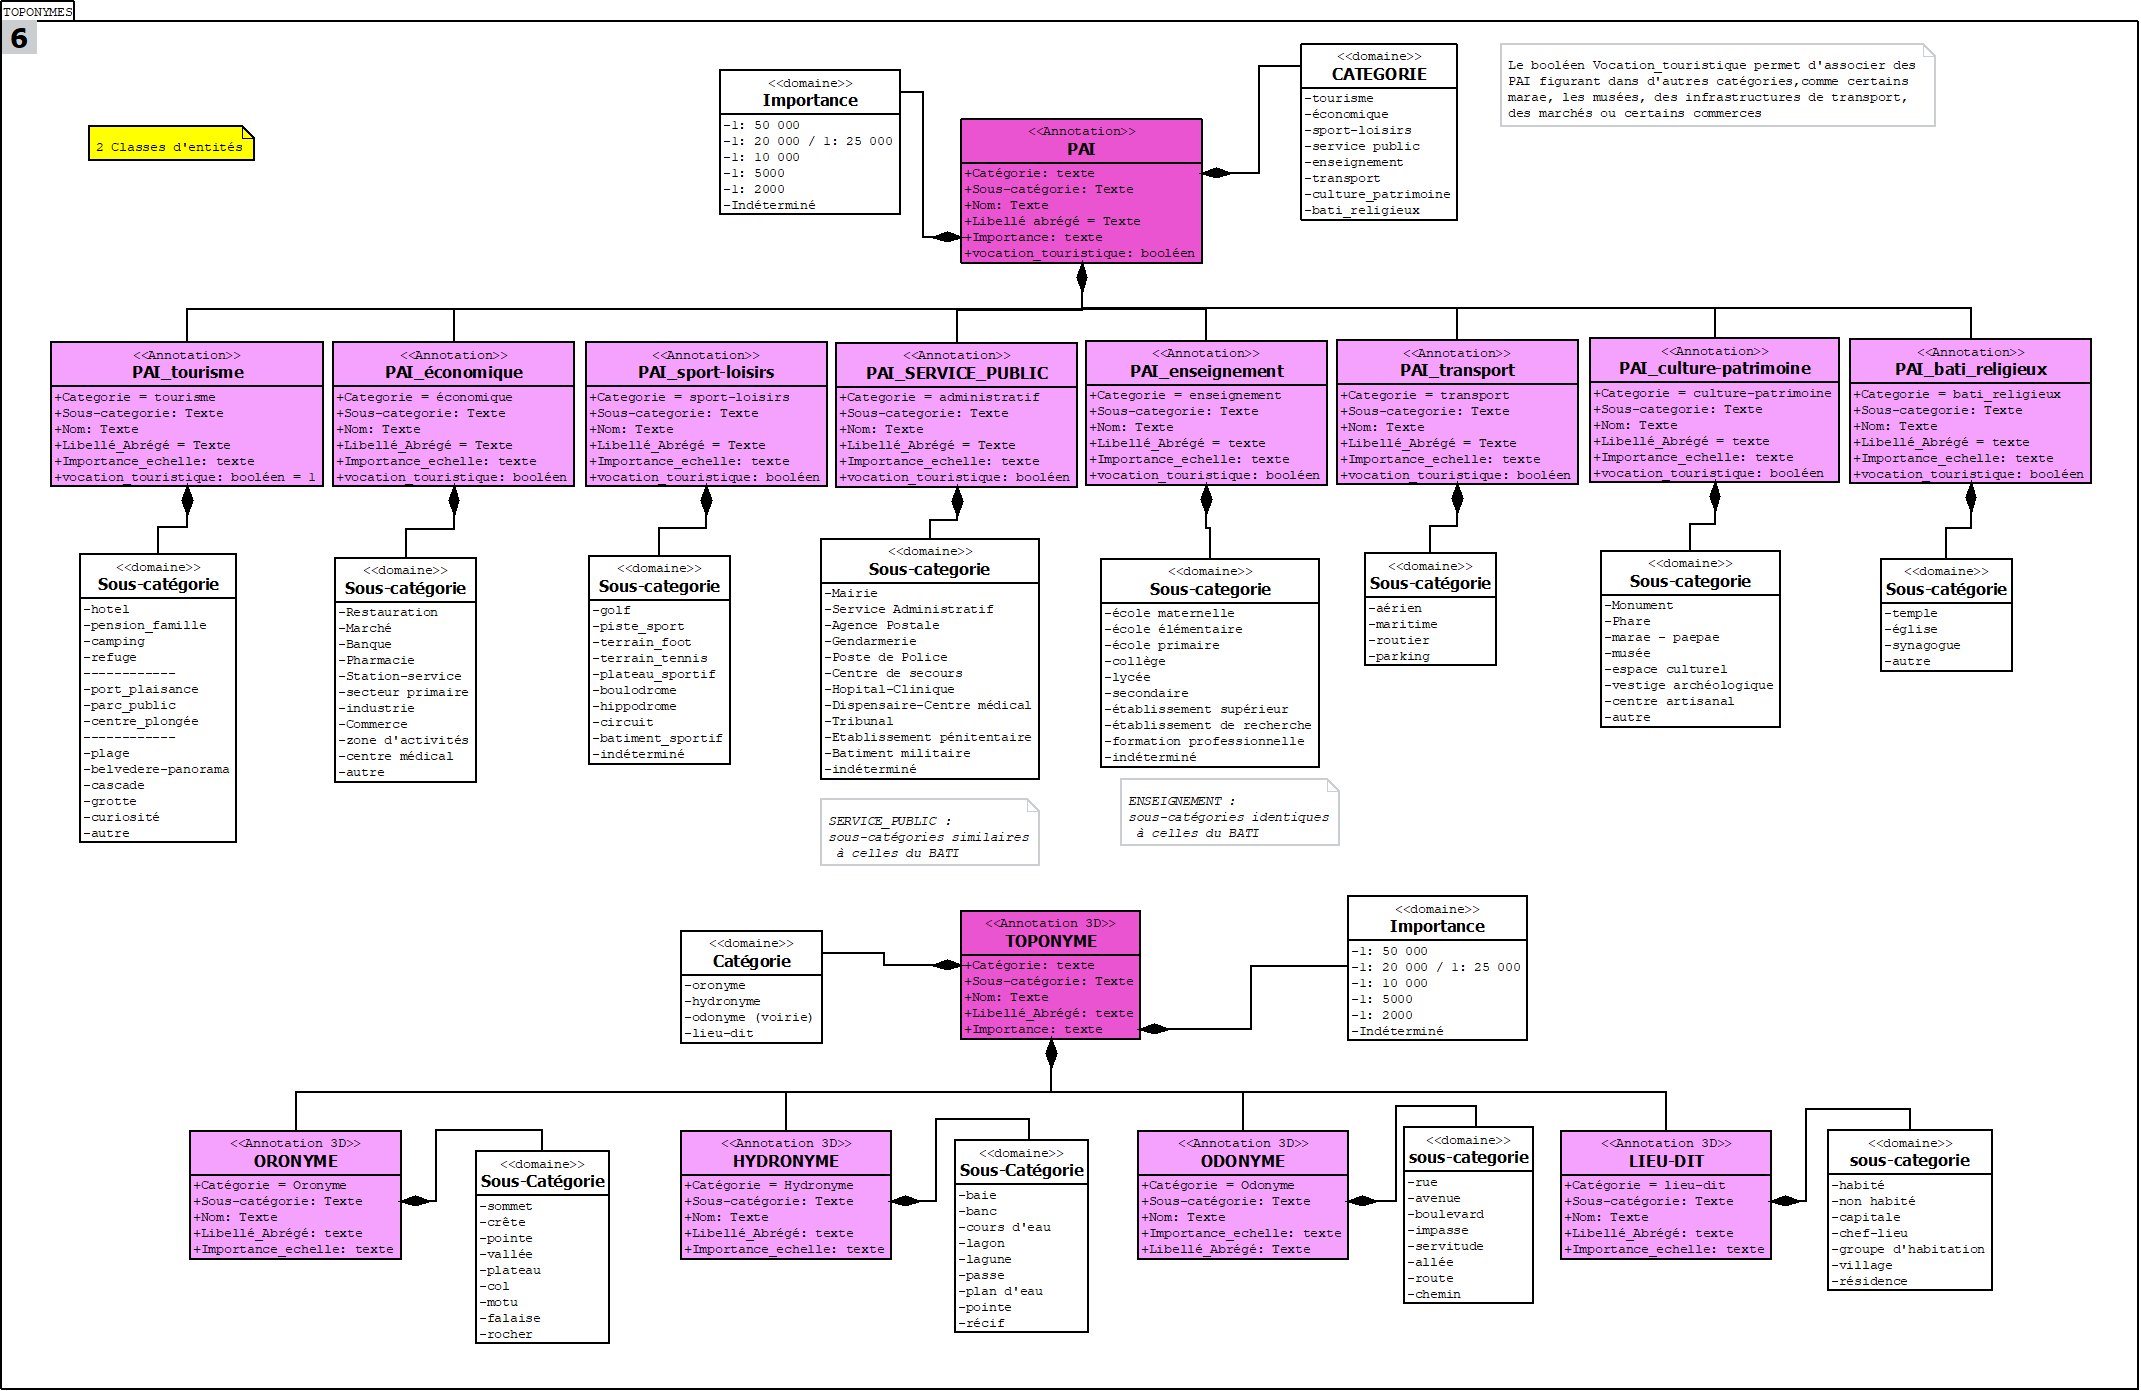
\includegraphics[width=\linewidth]{images/Architecture_BDD/NOM_TOPONYME-PAI.png}}%
\caption{Diagramme des classes servant à la toponymie}%
\textit{Il est à noter comme cela est précisé dans le rapport (page...) que ces classes comportent déjà un champ "Importance" avec des échelles et que ce champ permet de sélectionner pour une échelle donnée, les toponymes et autres points d'activités et d'intérêts (PAI) à placer sur la carte.}
\end{sidewaysfigure}

\addtocounter{figure}{-1}
\begin{sidewaysfigure}
\addtocounter{figure}{1}
\centering
\subfigure{%
\label{fig:graphics:b}% label for subfigure
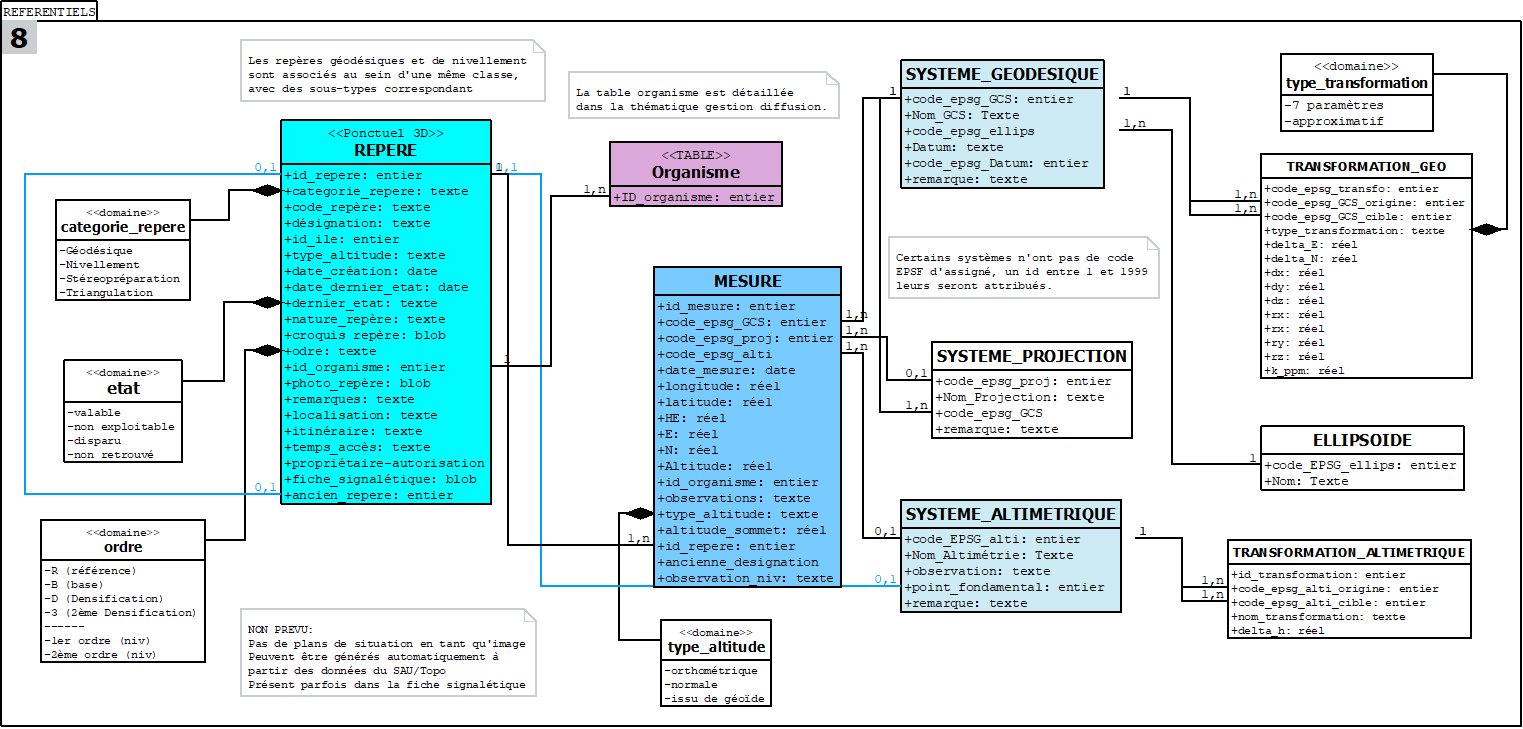
\includegraphics[width=\linewidth]{images/Architecture_BDD/REF_REFERENTIEL.png}}%
\caption{Diagramme des classes concernant le référentiel de mesure}%
\end{sidewaysfigure}

\addtocounter{figure}{-1}
\begin{sidewaysfigure}
\addtocounter{figure}{1}
\centering
\subfigure{%
\label{fig:graphics:b}% label for subfigure
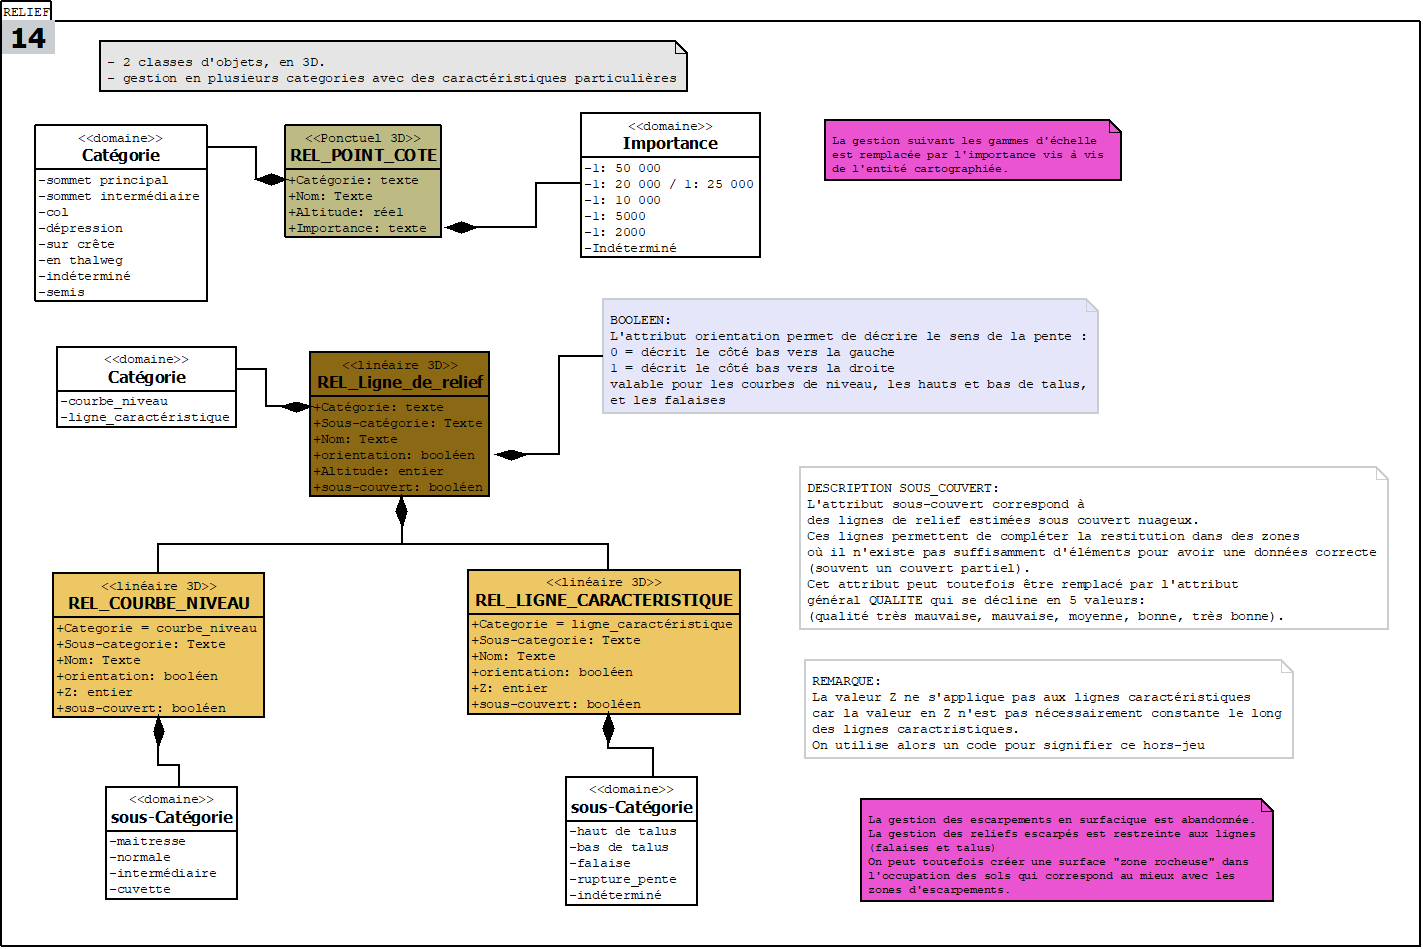
\includegraphics[width=\linewidth]{images/Architecture_BDD/REL_RELIEF.png}}%
\caption{Diagramme des classes concernant la thématique du relief}%
\end{sidewaysfigure}

\addtocounter{figure}{-1}
\begin{sidewaysfigure}
\addtocounter{figure}{1}
\centering
\subfigure{%
\label{fig:graphics:b}% label for subfigure
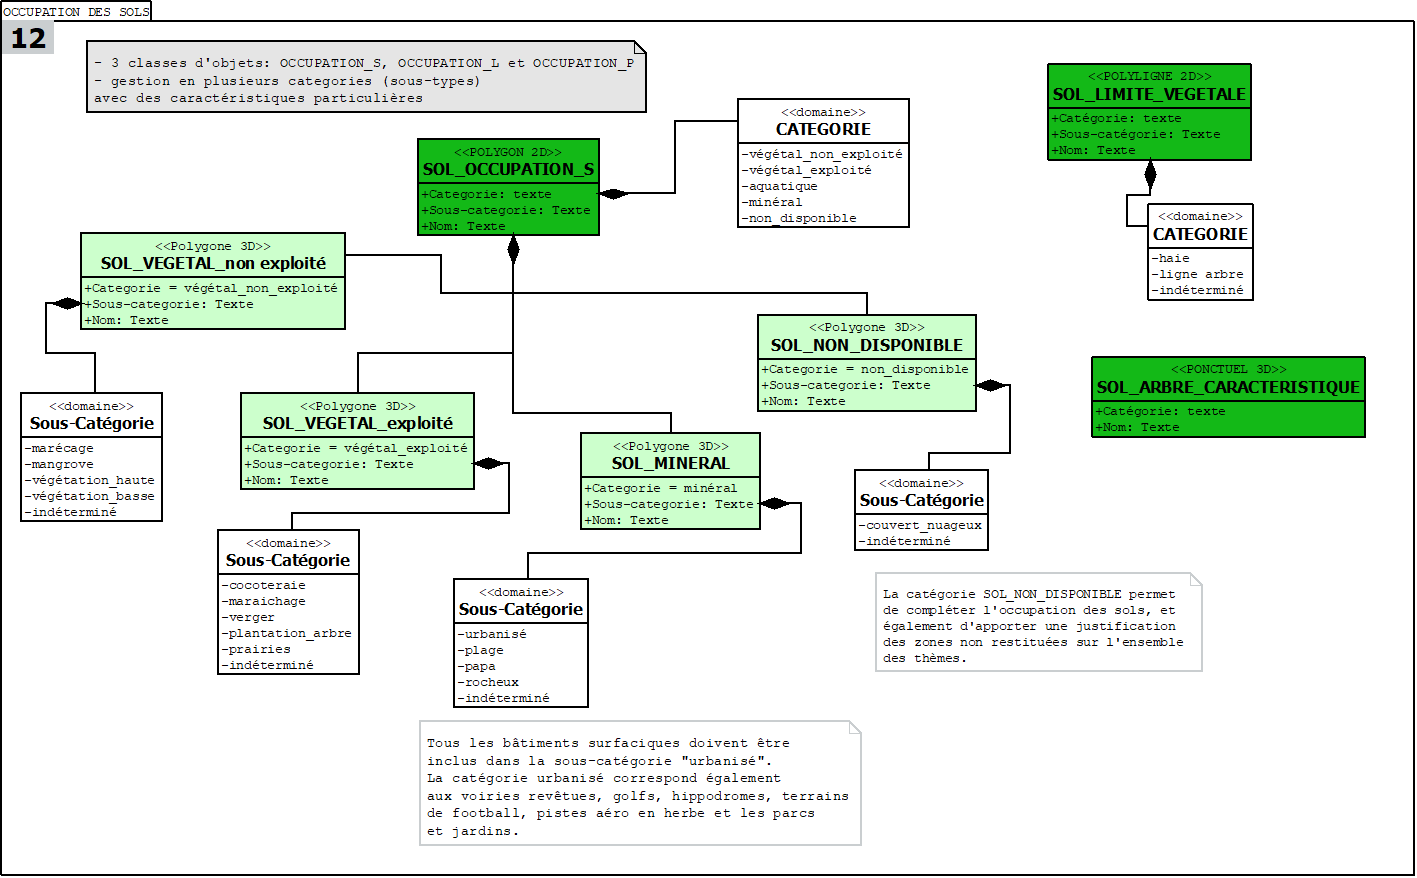
\includegraphics[width=\linewidth]{images/Architecture_BDD/SOL_OCCUPATION_SOLS.png}}%
\caption{Diagramme des classes concernant la thématique de l'occupation des sols}%
\end{sidewaysfigure}

\addtocounter{figure}{-1}
\begin{sidewaysfigure}
\addtocounter{figure}{1}
\centering
\subfigure{%
\label{fig:graphics:b}% label for subfigure
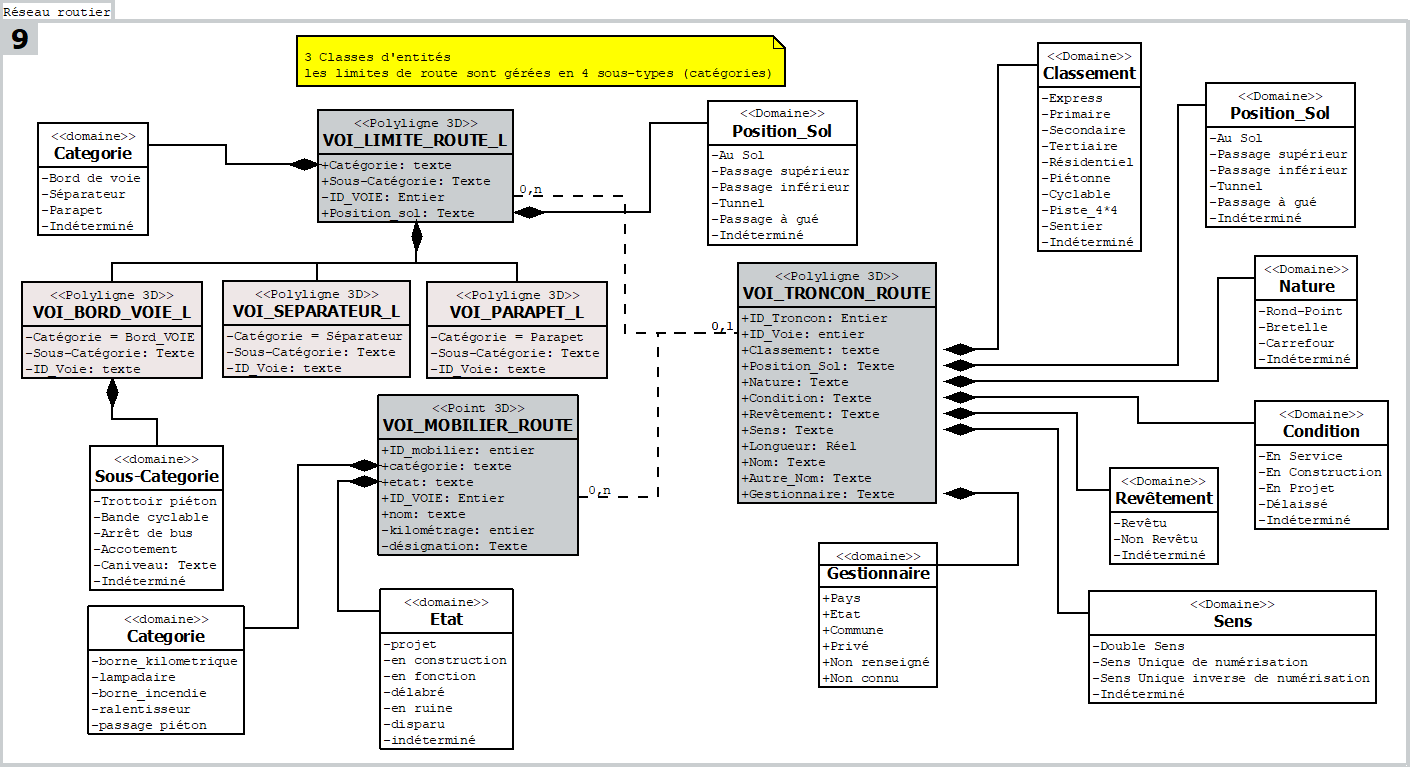
\includegraphics[width=\linewidth]{images/Architecture_BDD/VOI_RESEAU_ROUTIER.png}}%
\caption{Diagramme des classes concernant la thématique de la voirie}%
\end{sidewaysfigure}

\addtocounter{figure}{-1}
\begin{sidewaysfigure}
\addtocounter{figure}{1}
\centering
\subfigure{%
\label{fig:graphics:b}% label for subfigure
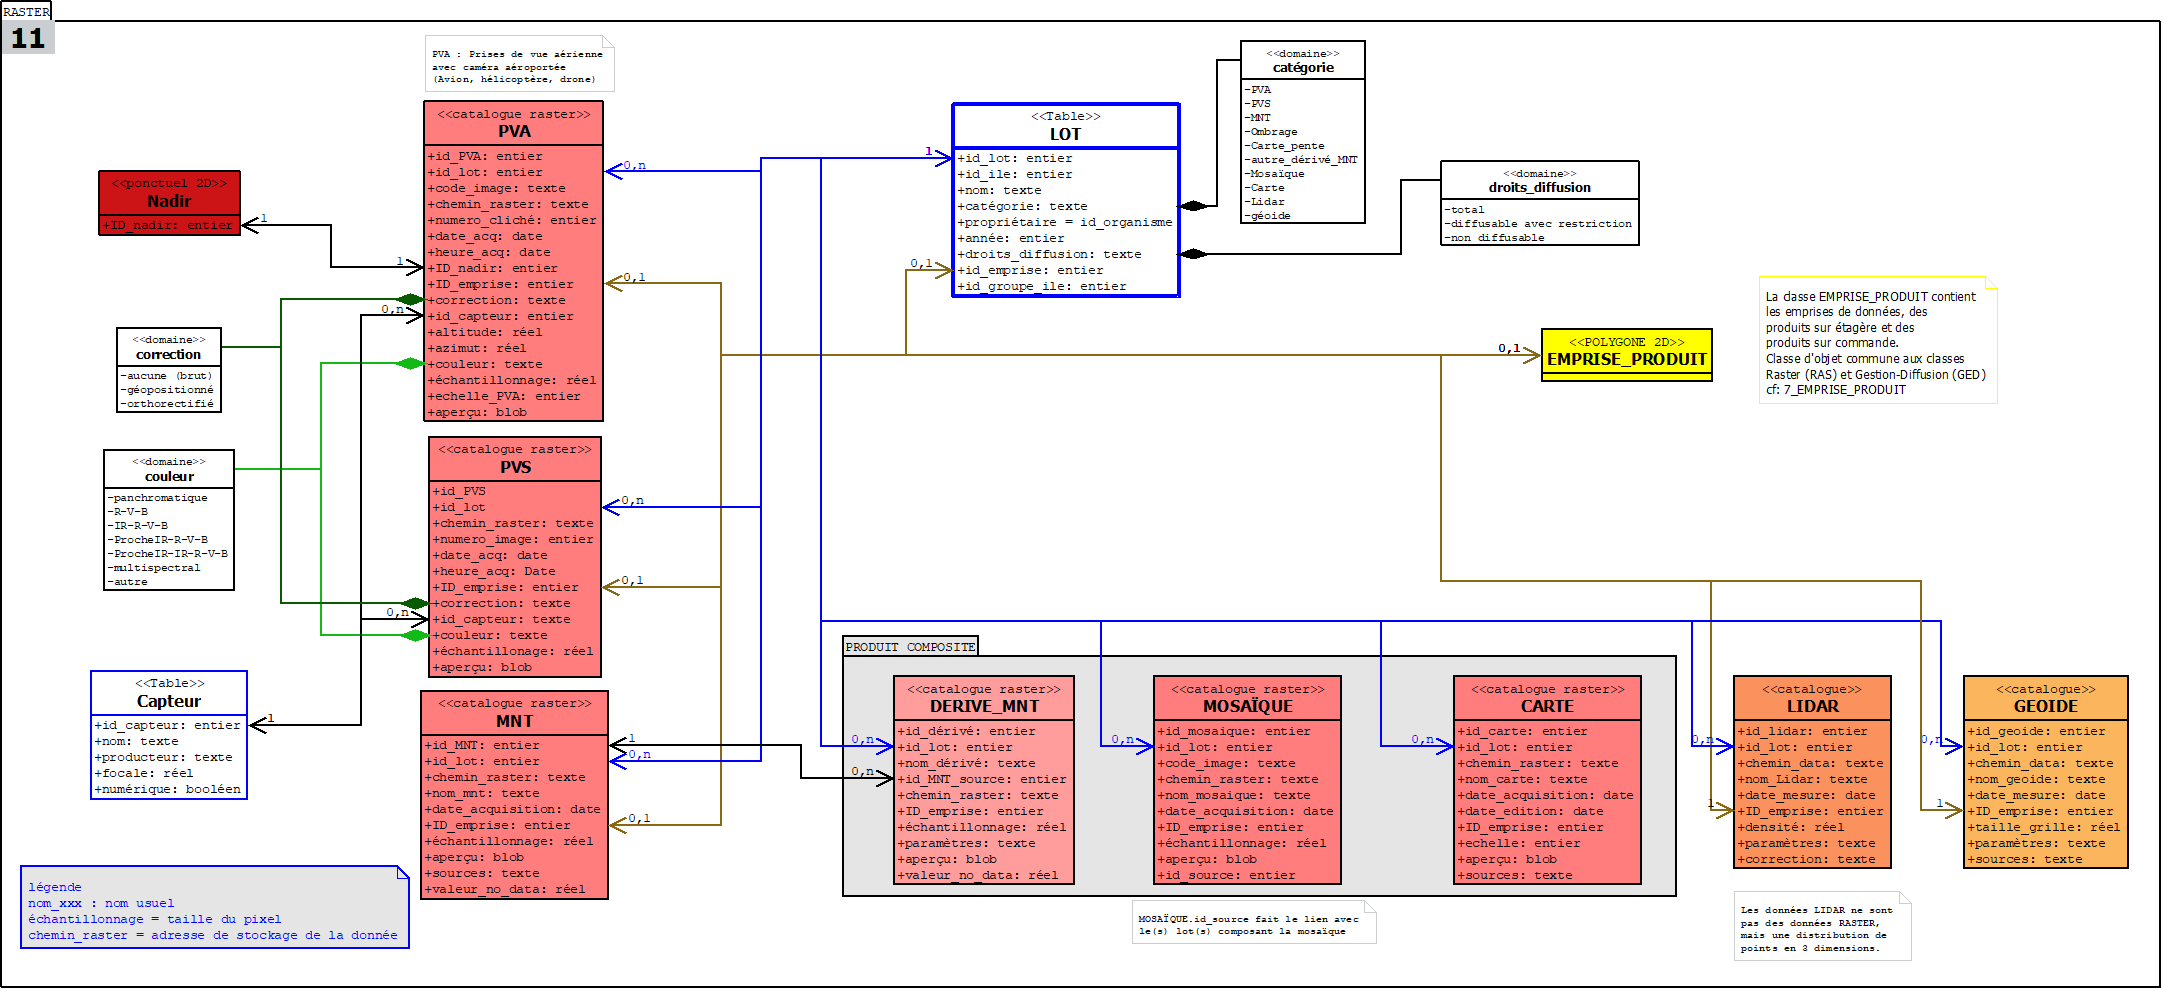
\includegraphics[width=\linewidth]{images/Architecture_BDD/RAS_RASTER.png}}%
\caption{Diagramme des classes présentant l'éventail des produits rasters}%
\end{sidewaysfigure}

%%%%%%%%%%%%%%%%%%%%%%%%%%%%%%%%%%%%%%%%%%%%%%%%%%%%%%%%%%%%%%%%%%%%%%%%%%
%%%%%%%%%%%%%%%%%%%%%   ANNEXE B  %%%%%%%%%%%%%%%%%%%%%%%%%%%%%%%%%%%%%%%%
%%%%%%%%%%%%%%%%%%%%%%%%%%%%%%%%%%%%%%%%%%%%%%%%%%%%%%%%%%%%%%%%%%%%%%%%%%
\annexe[Base de données de la Polynésie Française - Liste des classes et informations]{ Architecture de la base de Données de la Polynésie Française \newline \textit{Liste des classes et informations}}
\label{annexearchitecure}

\begin{table}[!h]

\begin{center}
    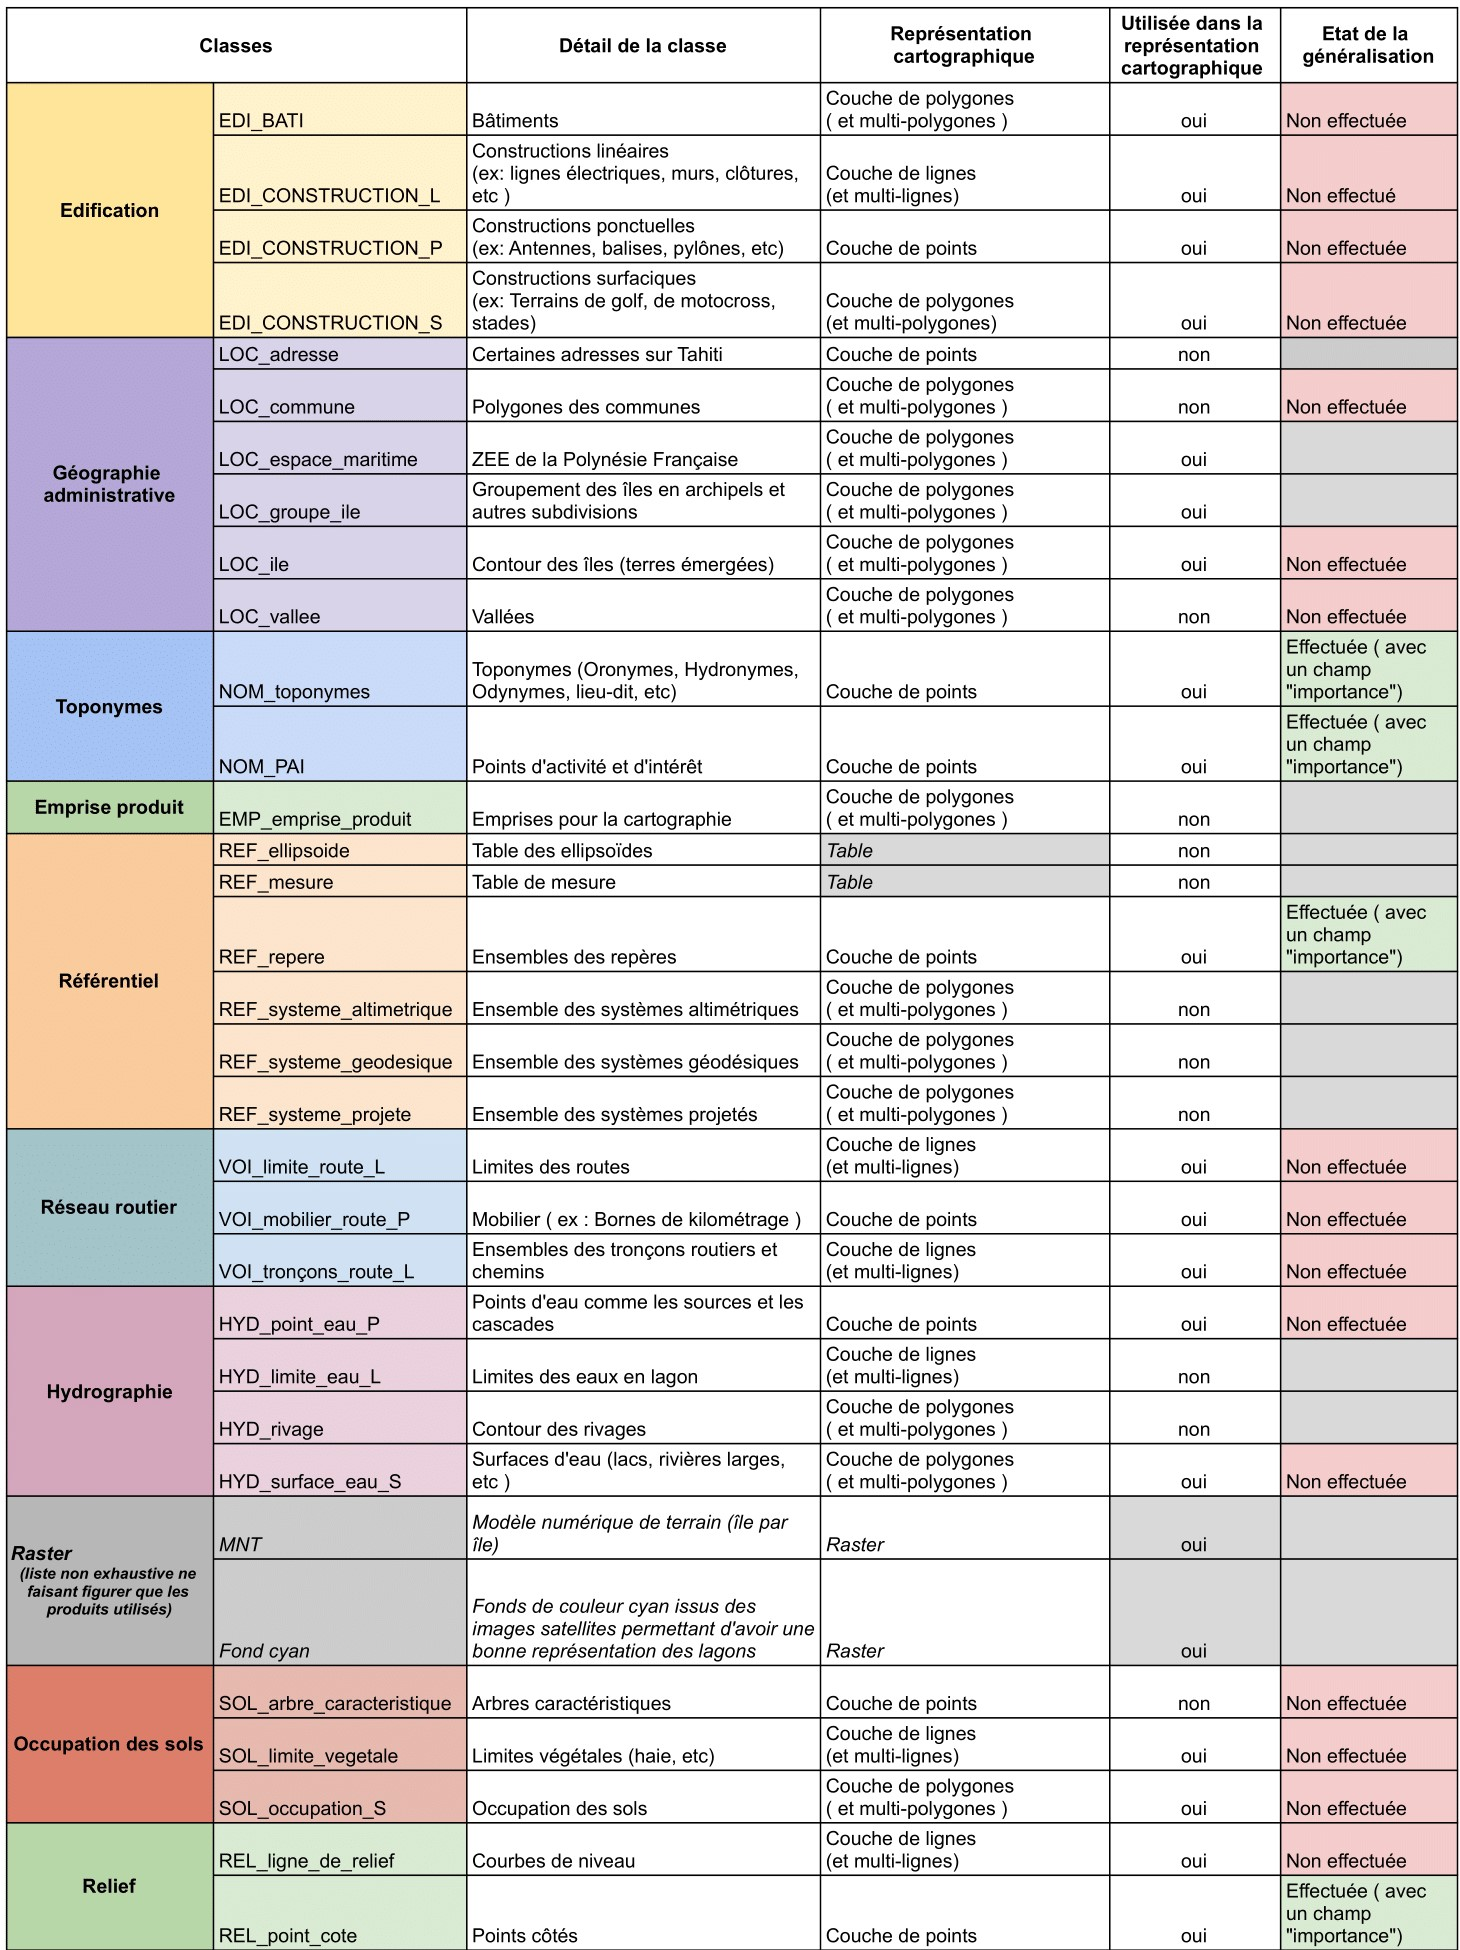
\includegraphics[width=11.95cm]{images/Annexes/table.jpg}%
    \label{fig:graphics:b}% label for subfigure
    \caption{Tableau récapitulatif des classes de la base de donnée et de leur état de généralisation avant le projet}
\end{center}

\end{table}

%%%%%%%%%%%%%%%%%%%%%%%%%%%%%%%%%%%%%%%%%%%%%%%%%%%%%%%%%%%%%%%%%%%%%%%%%%
%%%%%%%%%%%%%%%%%%%%%   ANNEXE C  %%%%%%%%%%%%%%%%%%%%%%%%%%%%%%%%%%%%%%%%
%%%%%%%%%%%%%%%%%%%%%%%%%%%%%%%%%%%%%%%%%%%%%%%%%%%%%%%%%%%%%%%%%%%%%%%%%%

\annexe[Répartition de la Polynésie Française en quatre fuseaux ]{ Répartition de la Polynésie Française en quatre fuseaux}
\label{annexefuseau}


\begin{figure}[!h]
\centering
\includegraphics[width=\linewidth]{images/chap0/PF_carte_generale_UTM_90x90_2012-1.png}
\caption{Carte des fuseaux UTM de la Polynésie Française - Produit de la section topographie - 2012}
\label{fuseauUTM}
\end{figure}



%%%%%%%%%%%%%%%%%%%%%%%%%%%%%%%%%%%%%%%%%%%%%%%%%%%%%%%%%%%%%%%%%%%%%%%%%%
%%%%%%%%%%%%%%%%%%%%%   ANNEXE D  %%%%%%%%%%%%%%%%%%%%%%%%%%%%%%%%%%%%%%%%
%%%%%%%%%%%%%%%%%%%%%%%%%%%%%%%%%%%%%%%%%%%%%%%%%%%%%%%%%%%%%%%%%%%%%%%%%%

%% Mise en forme des txt %%
\makeatletter
\newcommand\verbfile[1]{%
	\begingroup
		\let\do\@makeother\dospecials
		\obeyspaces\ttfamily
		\catcode`\^^M\active
		\begingroup\lccode`\~`\^^M \lowercase{\endgroup\def~{\par\leavevmode}}%
		\input#1\relax
	\endgroup
}
\makeatother

%% ___________________________________
 

\annexe[Détail des traitements réalisés sur les couches]{Détail des traitements réalisés sur les couches}
\label{annexemodelbuilder}

%-----------------------------

\begin{center}
    \Large
    \textbf{EDI\_BATI}
\end{center}

\verbfile{README_TXT/README_EDI_Bati.txt}

\begin{sidewaysfigure}
\centering
\subfigure{%
\label{fig:graphics:a}% label for subfigure
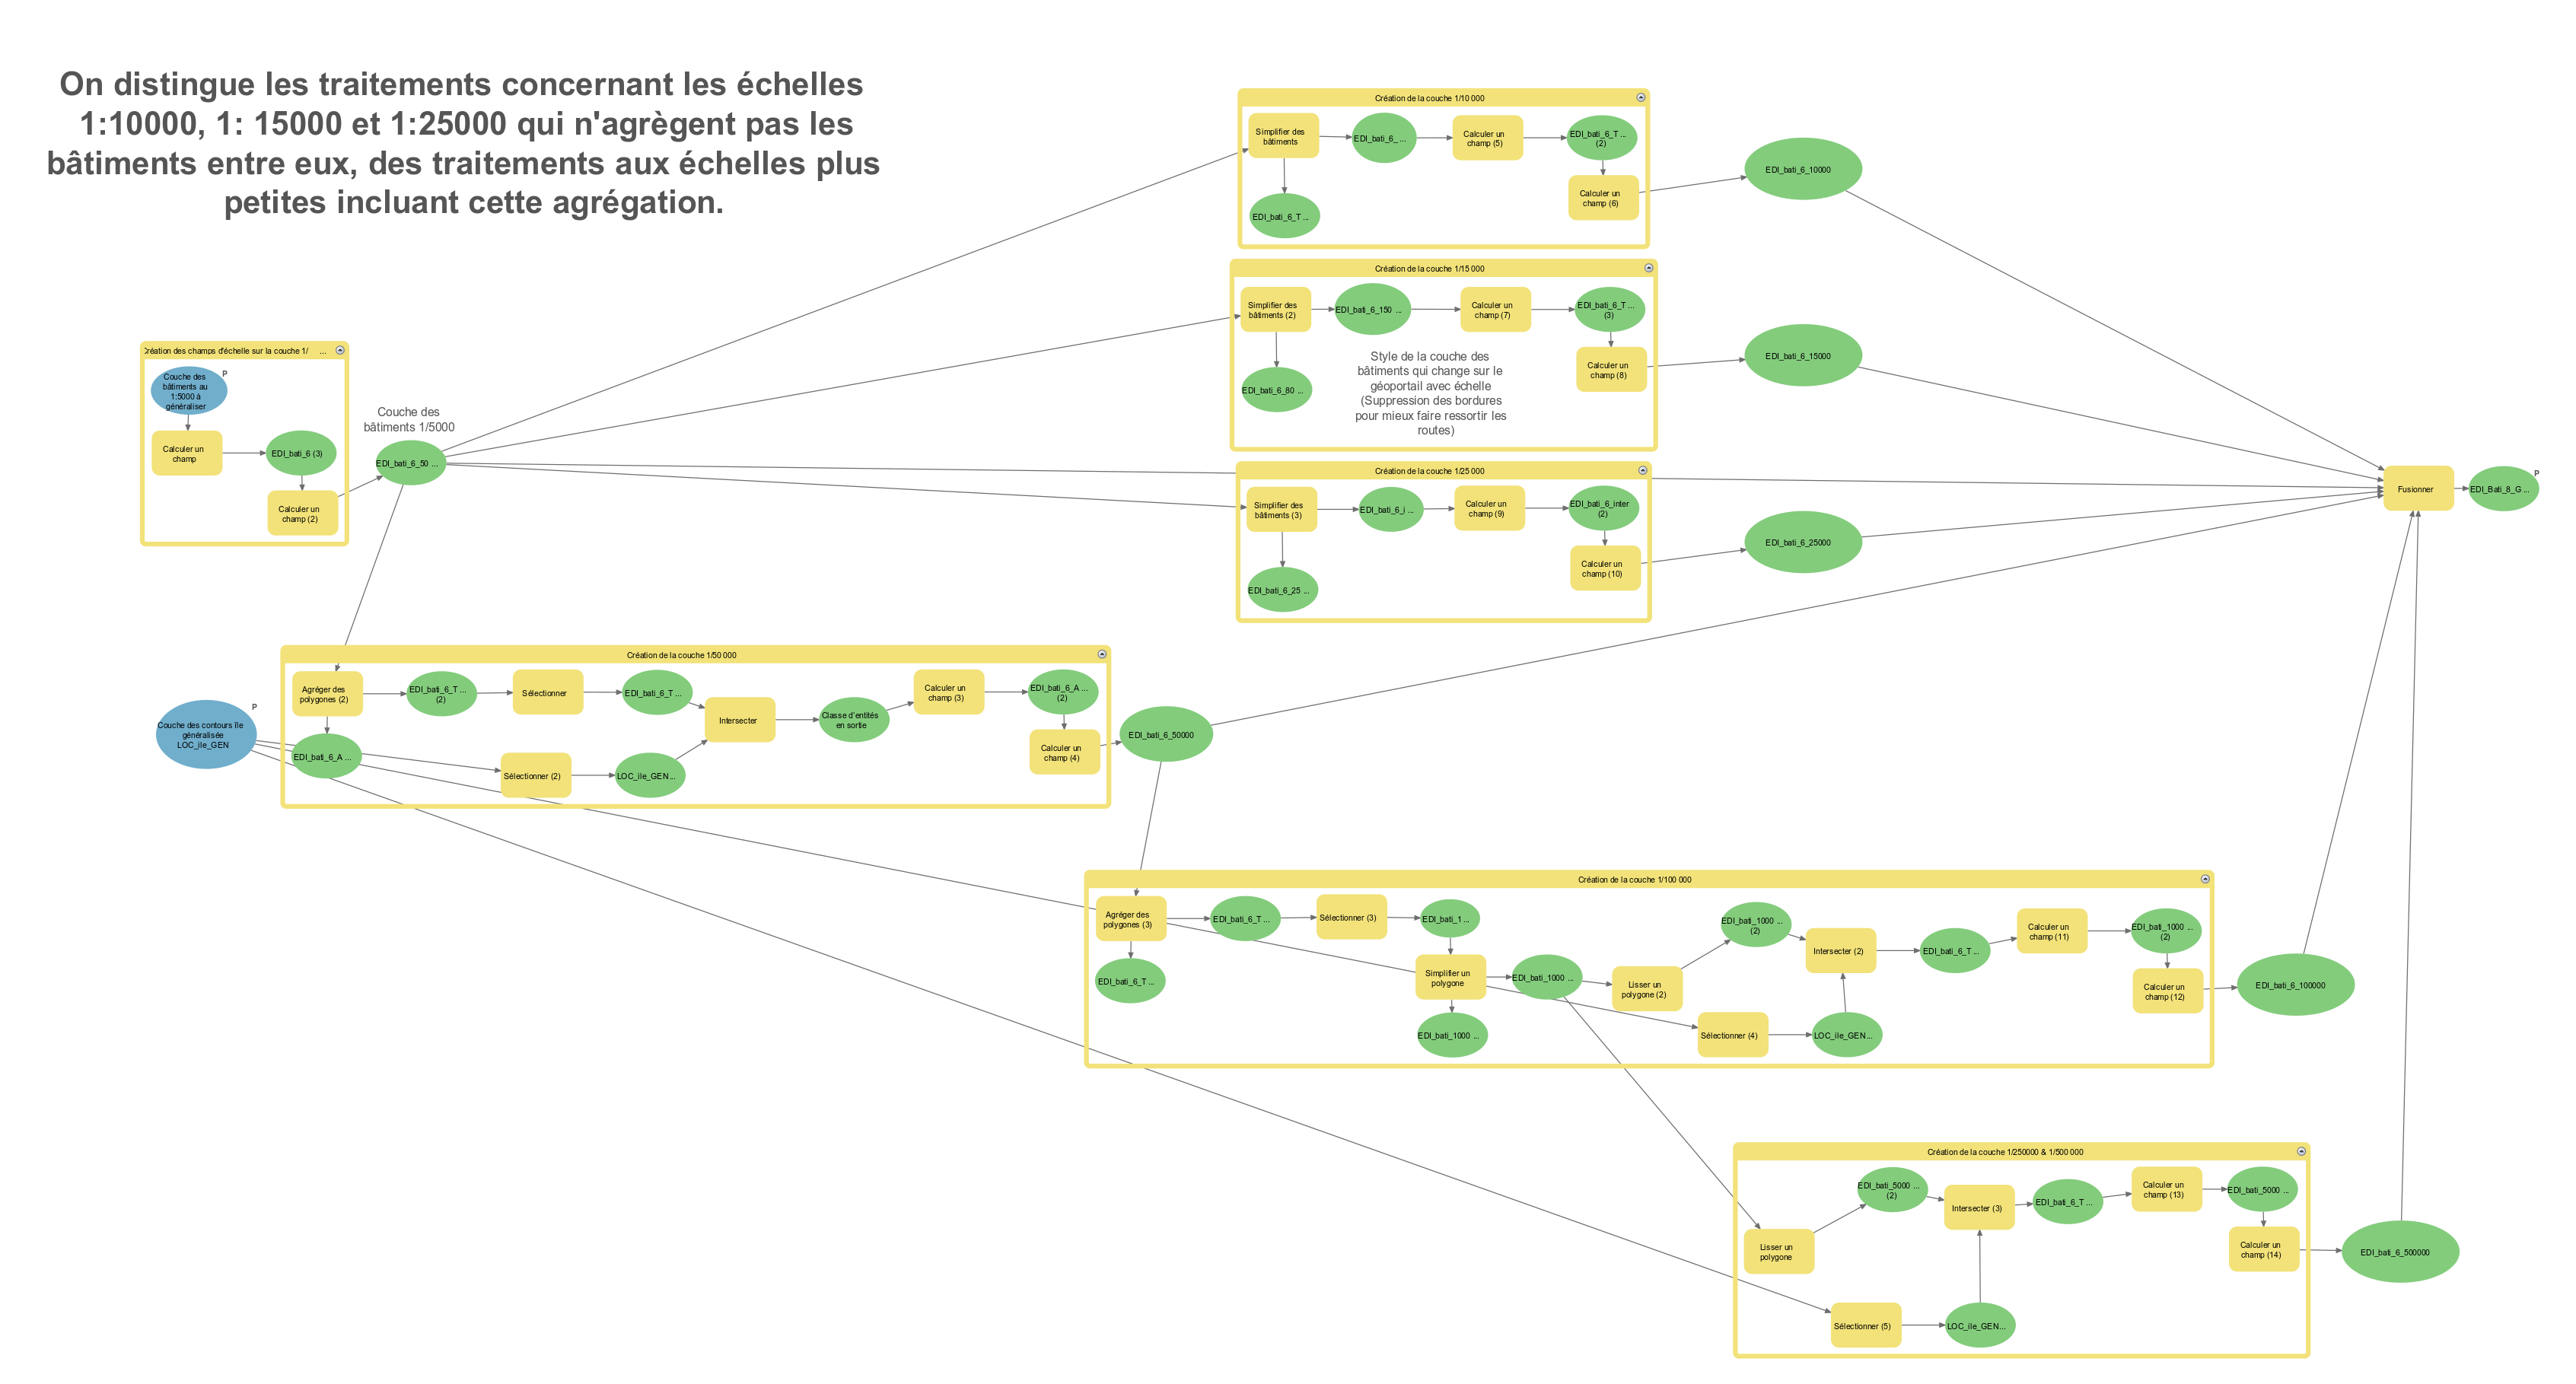
\includegraphics[width=\linewidth]{images/Annexes/modelbuilder/Modele_EDI_BATI.png}}%
\caption{ModelBuilder d'ArcGIS pour le traitement des couches de bâtiments}%
\textit{Commentaire éventuel}
\label{fig:graphics}% label for figure
\end{sidewaysfigure}


\clearpage
% ---------------------------


\begin{center}
    \Large
    \textbf{EDI\_CONSTRUCTION\_S}
\end{center}

\verbfile{README_TXT/README_EDI_construction_S.txt}

\addtocounter{figure}{-1}
\begin{figure}
\addtocounter{figure}{1}
\centering
\subfigure{%
\label{fig:graphics:b}% label for subfigure
\includegraphics[width=\linewidth]{images/Annexes/modelbuilder/Modèle_EDI_CONSTRUCTION_S.png}}%
\caption{ModelBuilder d'ArcGIS pour le traitement des couches de constructions surfaciques}%
\textit{Commentaire éventuel}
\end{figure}


\clearpage
% ---------------------------


\begin{center}
    \Large
    \textbf{LOC\_ile}
\end{center}

\verbfile{README_TXT/README_LOC_ile.txt}

\addtocounter{figure}{-1}
\begin{sidewaysfigure}
\addtocounter{figure}{1}
\centering
\subfigure{%
\label{fig:graphics:b}% label for subfigure
\includegraphics[width=\linewidth]{images/Annexes/modelbuilder/Modèle_LOC_ILE.png}}%
\caption{ModelBuilder d'ArcGIS pour le traitement des couches de contour des îles}%
\textit{Commentaire éventuel}
\end{sidewaysfigure}


\clearpage
% ---------------------------


\begin{center}
    \Large
    \textbf{LOC\_limite\_commune}
\end{center}

\verbfile{README_TXT/README_LOC_limite_commune.txt}

\addtocounter{figure}{-1}
\begin{sidewaysfigure}
\addtocounter{figure}{1}
\centering
\subfigure{%
\label{fig:graphics:b}% label for subfigure
\includegraphics[width=\linewidth]{images/Annexes/modelbuilder/Modèle_LOC_ILE.png}}%
\caption{ModelBuilder d'ArcGIS pour le traitement des couches de contour des communes}%
\textit{Commentaire éventuel}
\end{sidewaysfigure}


\clearpage
% ---------------------------

\begin{center}
    \Large
    \textbf{REL\_ligne\_relief}
\end{center}

\verbfile{README_TXT/README_REL_ligne_relief.txt}

\addtocounter{figure}{-1}
\begin{sidewaysfigure}
\addtocounter{figure}{1}
\centering
\subfigure{%
\label{fig:graphics:b}% label for subfigure
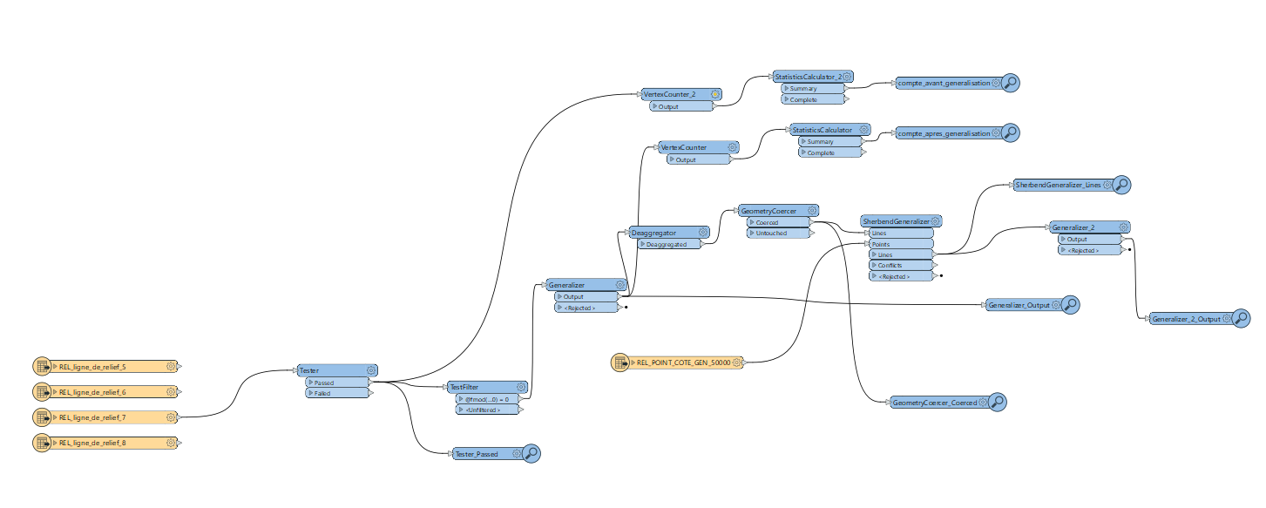
\includegraphics[width=\linewidth]{images/Annexes/modelbuilder/fme_REL_ligne de relief.png}}%
\caption{ModelBuilder d'ArcGIS pour le traitement des couches de contour des communes}%
\textit{Commentaire éventuel}
\end{sidewaysfigure}


% ---------------------------


%%%%%%%%%%%%%%%%%%%%%%%%%%%%%%%%%%%%%%%%%%%%%%%%%%%%%%%%%%%%%%%%%%%%%%%%%%
%%%%%%%%%%%%%%%%%%%%%   ANNEXE XX  %%%%%%%%%%%%%%%%%%%%%%%%%%%%%%%%%%%%%%%%
%%%%%%%%%%%%%%%%%%%%%%%%%%%%%%%%%%%%%%%%%%%%%%%%%%%%%%%%%%%%%%%%%%%%%%%%%%
\annexe[Carte IGN 1988 Echelle 1/100 000]{ Carte IGN 1988 Echelle 1/100 000}
\label{annexeign88}

\begin{figure}[!h]
\centering
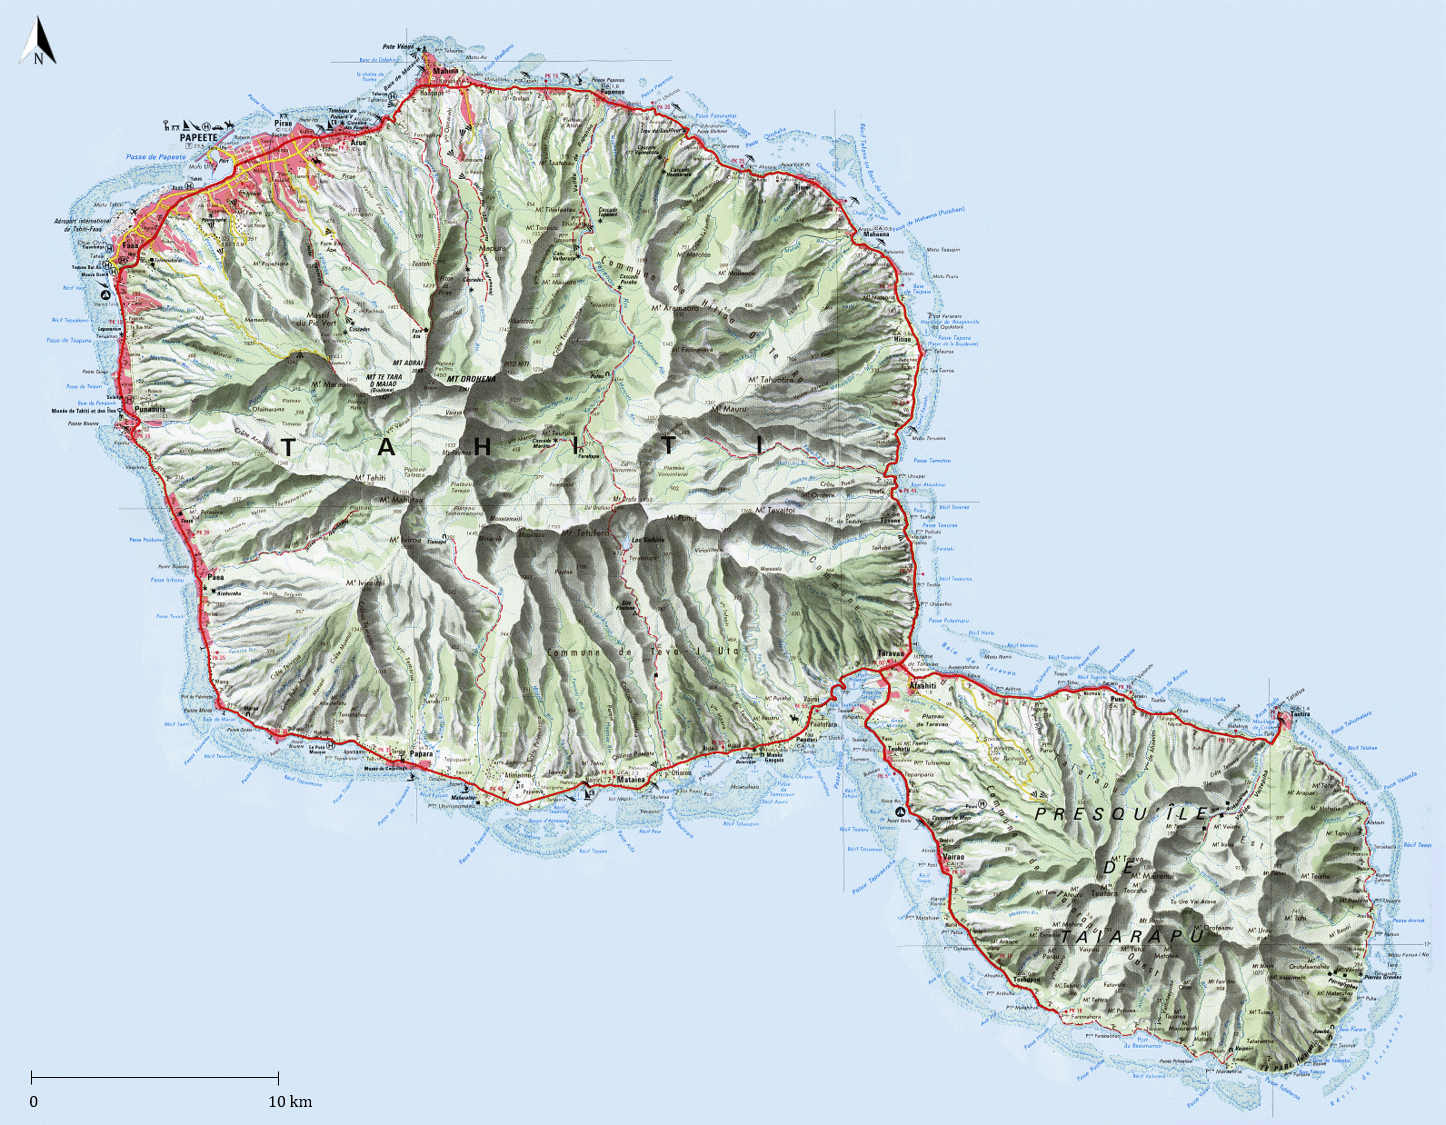
\includegraphics[width=\linewidth]{images/Annexes/tahiti_ign_1988.png}%
\caption{Carte réalisée par l'IGN en 1988 à l'échelle 1/100 000}%
\label{carte1988}% label for figure
\end{figure}


\definecolor{darkWhite}{rgb}{0.94,0.94,0.94}

%%%%%%%%%%%%%%%%%%%%%%%%%%%%%%%%%%%%%%%%%%%%%%%%%%%%%%%%%%%%%%%%%%%%%%%%%%
%%%%%%%%%%%%%%%%%%%%%   ANNEXE XX  %%%%%%%%%%%%%%%%%%%%%%%%%%%%%%%%%%%%%%%%
%%%%%%%%%%%%%%%%%%%%%%%%%%%%%%%%%%%%%%%%%%%%%%%%%%%%%%%%%%%%%%%%%%%%%%%%%%
\annexe[Classement des récifs coralliens de la Polynésie Française]{ Classement des récifs coralliens de la Polynésie Française}
\label{annexecorail}

\begin{figure}[!h]
\centering
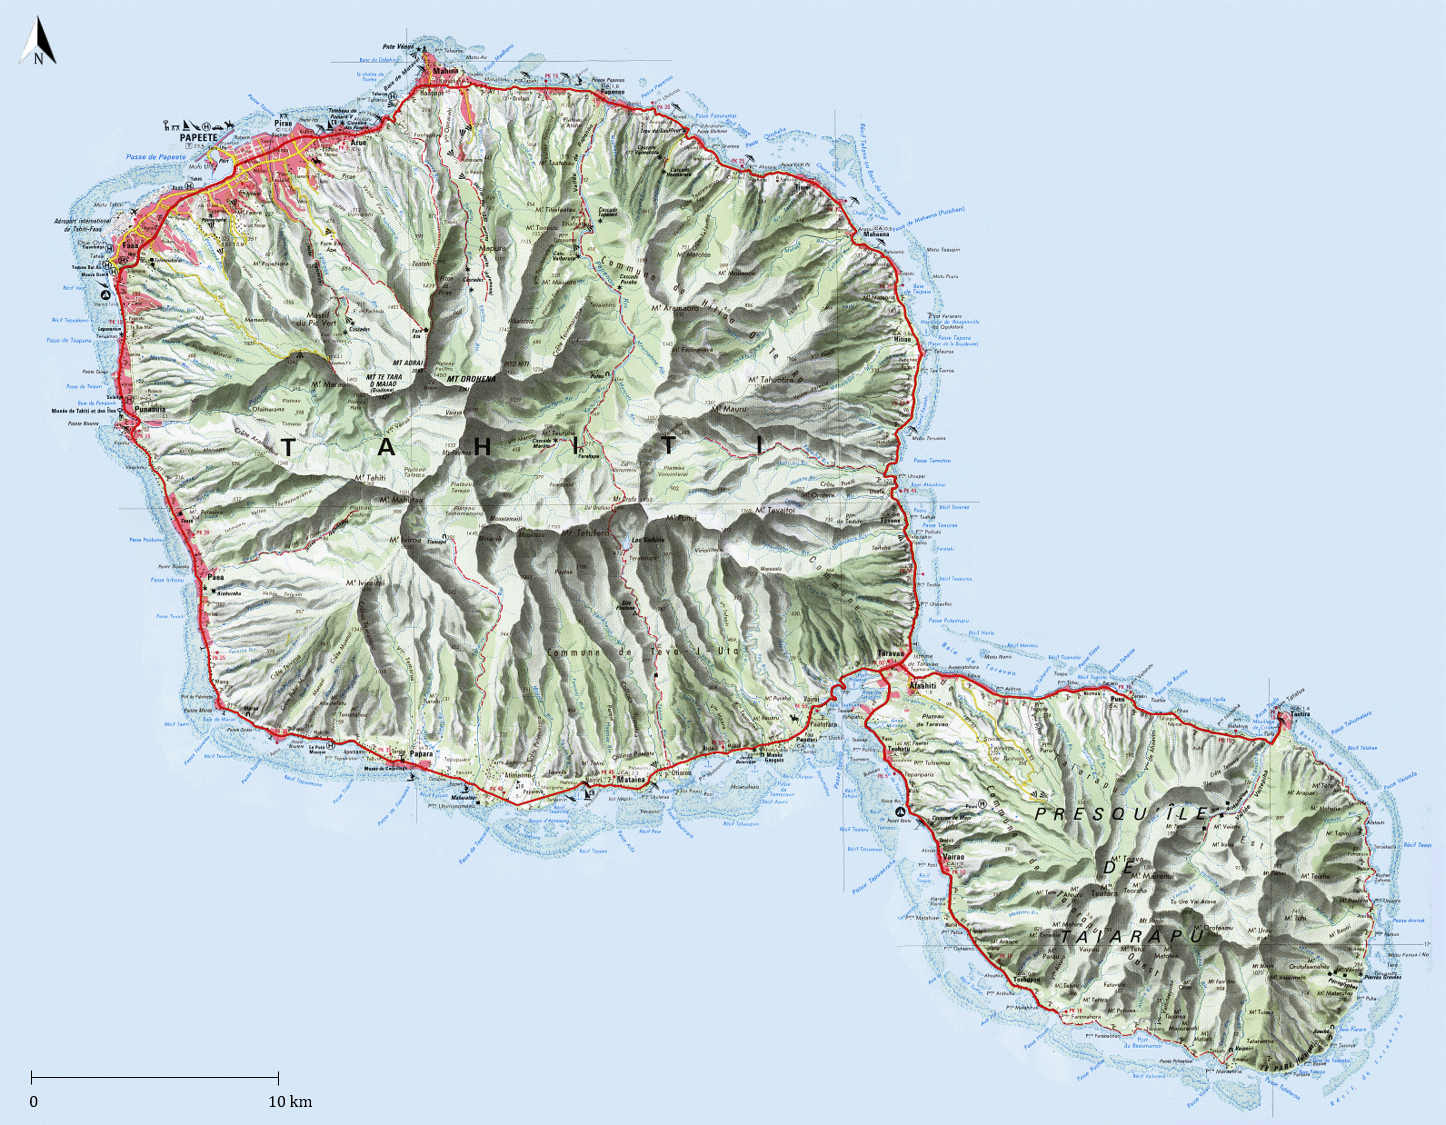
\includegraphics[width=\linewidth]{images/Annexes/tahiti_ign_1988.png}%
\caption{Carte réalisée par l'IGN en 1988 à l'échelle 1/100 000}%
\label{carte1988}% label for figure
\end{figure}


\definecolor{darkWhite}{rgb}{0.94,0.94,0.94}


%%%%%%%%%%%%%%%%%%%%%%%%%%%%%%%%%%%%%%%%%%%%%%%%%%%%%%%%%%%%%%%%%%%%%%%%%%
%%%%%%%%%%%%%%%%%%%%%   ANNEXE XX  %%%%%%%%%%%%%%%%%%%%%%%%%%%%%%%%%%%%%%%%
%%%%%%%%%%%%%%%%%%%%%%%%%%%%%%%%%%%%%%%%%%%%%%%%%%%%%%%%%%%%%%%%%%%%%%%%%%
\annexe[Quelques cartes topographiques avant la diffusion web]{ Quelques cartes topographiques avant la diffusion web}
\label{annexeresultat}

 
\begin{center}
\large
    \textbf{\textit{Préambule}}
\end{center}

Comme cela a été précisé dans le rapport, ces échantillons produits pour chaque échelle avaient pour objectif d'être imprimés au format A0 pour permettre de visualiser le rendu cartographique, d'en distinguer les potentielles erreurs, et de pouvoir corriger certains éléments. De plus, ces cartes au format A0 ont permis à l'ensemble des membres de la section topographie de faire leur retour et pouvoir ainsi améliorer au mieux la cartographie. Cette annexe permet de voir ces résultats. Cependant, les images affichés sont des cartes au format A0 réduites pour tenir sur une page A4. Elles sont donc difficilement lisibles mais donnent tout de même un aperçu des produits papiers réalisés au cours de ce stage avec leur emprise et c'est en cela qu'elles sont intéressantes. Pour permettre la lecture des cartes avec leur légende, des zones ont été sélectionnées et un grossissement a été réalisé. La figure ci-dessous répertorie les éléments de cette annexe pour une échelle donnée.\\

\begin{figure}[!h]
\centering
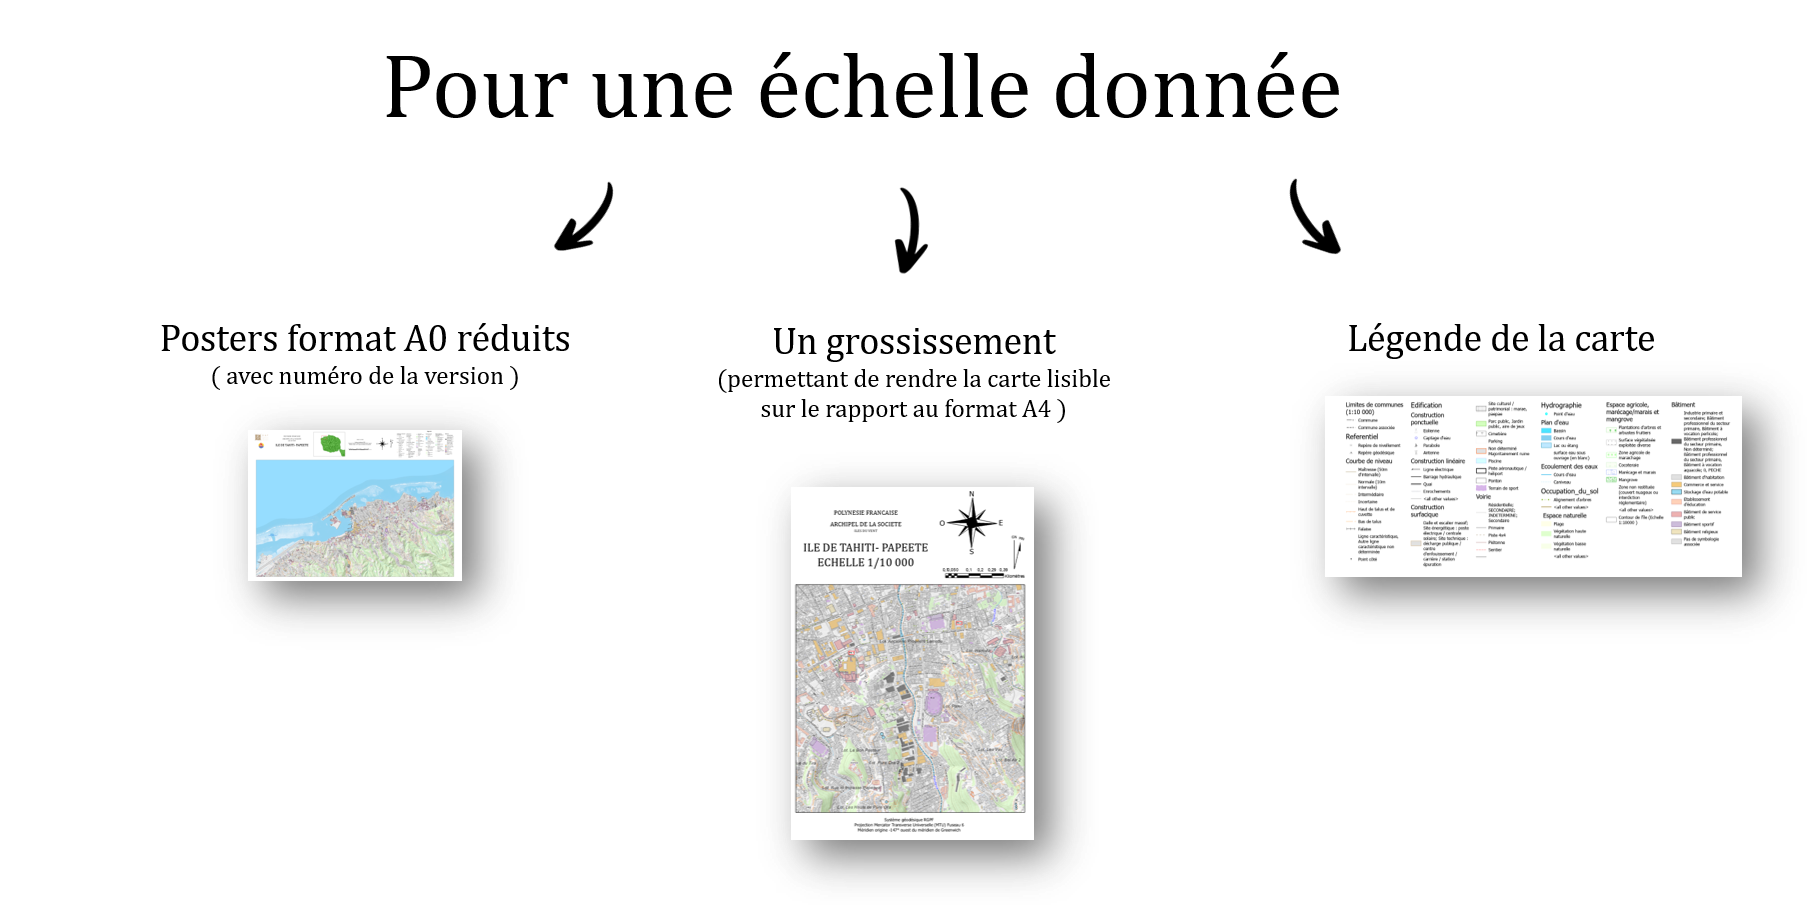
\includegraphics[width=\linewidth]{images/Annexes/Resultat/resultat_explication.png}%
\caption{Inventaire des éléments de cette annexe pour une échelle donnée}

\label{inventaire}% label for figure
\end{figure}

\textsc{Remarques}:\\
Les zooms effectués sur les cartes n'ont vocation qu'à rendre les objets cartographiques lisibles. L'impression au format A4 de ce rapport ne donnera pas un aperçu de la réalité. Par exemple un grossissement de la carte au 1/25 000 la rendant visible sur ce rapport ne signifie pas qu'une fois imprimée, un cm sur la carte correspondra à 25 000 cm sur la réalité. Il faut se référer à la barre d'échelle associée.


%%%%%%%%%%%%%%%%%%%%%%%%%


\begin{center}
    \Large
    \colorbox{blue!10}{--------------\- Echelle 1/10 000 --------------\-}
\end{center}


\begin{figure}[!h]
\centering
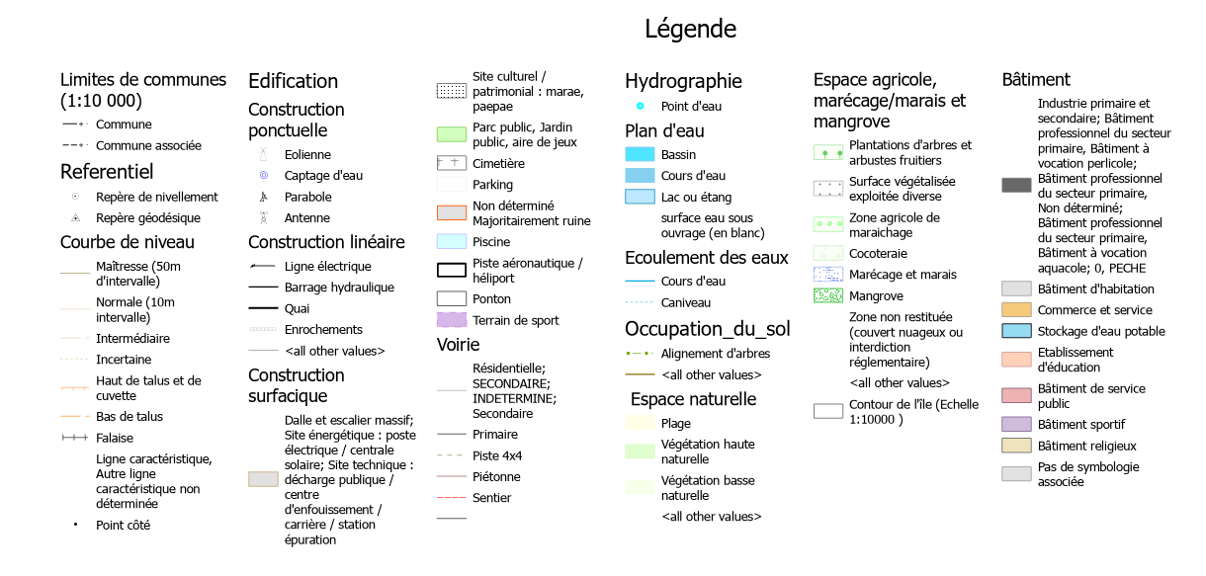
\includegraphics[width=\linewidth]{images/Annexes/Resultat/lengende_10.png}
\caption{Légende de la carte au 1/10 000}
\label{10000_legende}
\end{figure}

\vspace{3cm}
\textsc{Commentaires sur la carte au 1/10 000 :}\\
bornes pk,  quais etc etc

\begin{figure}[!h]
\centering
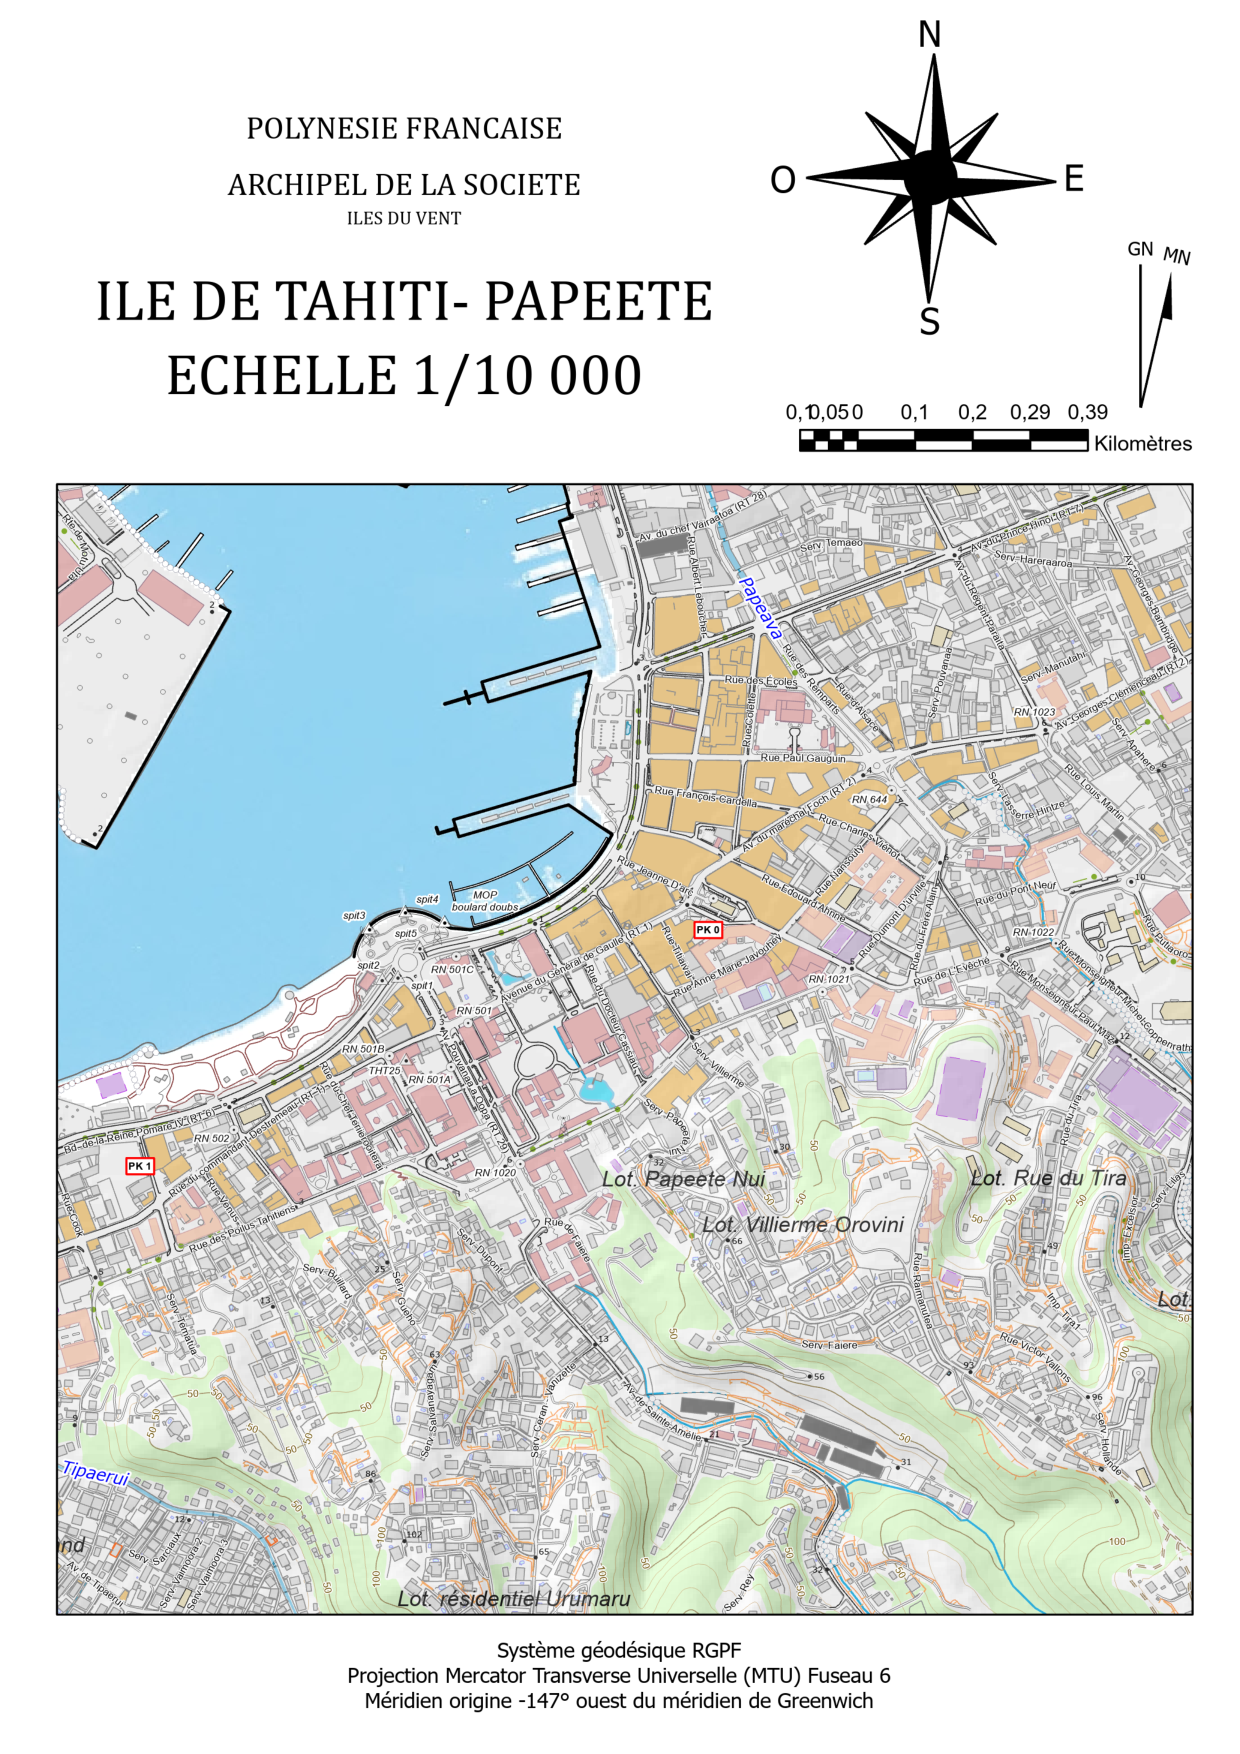
\includegraphics[width=\linewidth]{images/Annexes/Resultat/Carte_10000_A4.pdf}
\caption{Grossissement de la carte au 1/10 000 centrée sur le port de Papeete}
\label{10000_gros}
\end{figure}

\begin{sidewaysfigure}[!h]
\centering
\includegraphics[width=\linewidth]{images/Annexes/Resultat/Carte_10000.pdf}%
\caption{Poster format A0 réduit\color{red}{ Version 1}}
\colorbox{blue!10}{Echelle 1/10 000}
\label{10000}% label for figure
\end{sidewaysfigure}

\clearpage
%%%%%%%%%%%%%%%%%%%%%%%%%%%
\begin{center}
    \Large
    \colorbox{yellow!10}{--------------\- Echelle 1/15 000 --------------\-}
\end{center}

\begin{figure}[!h]
\centering
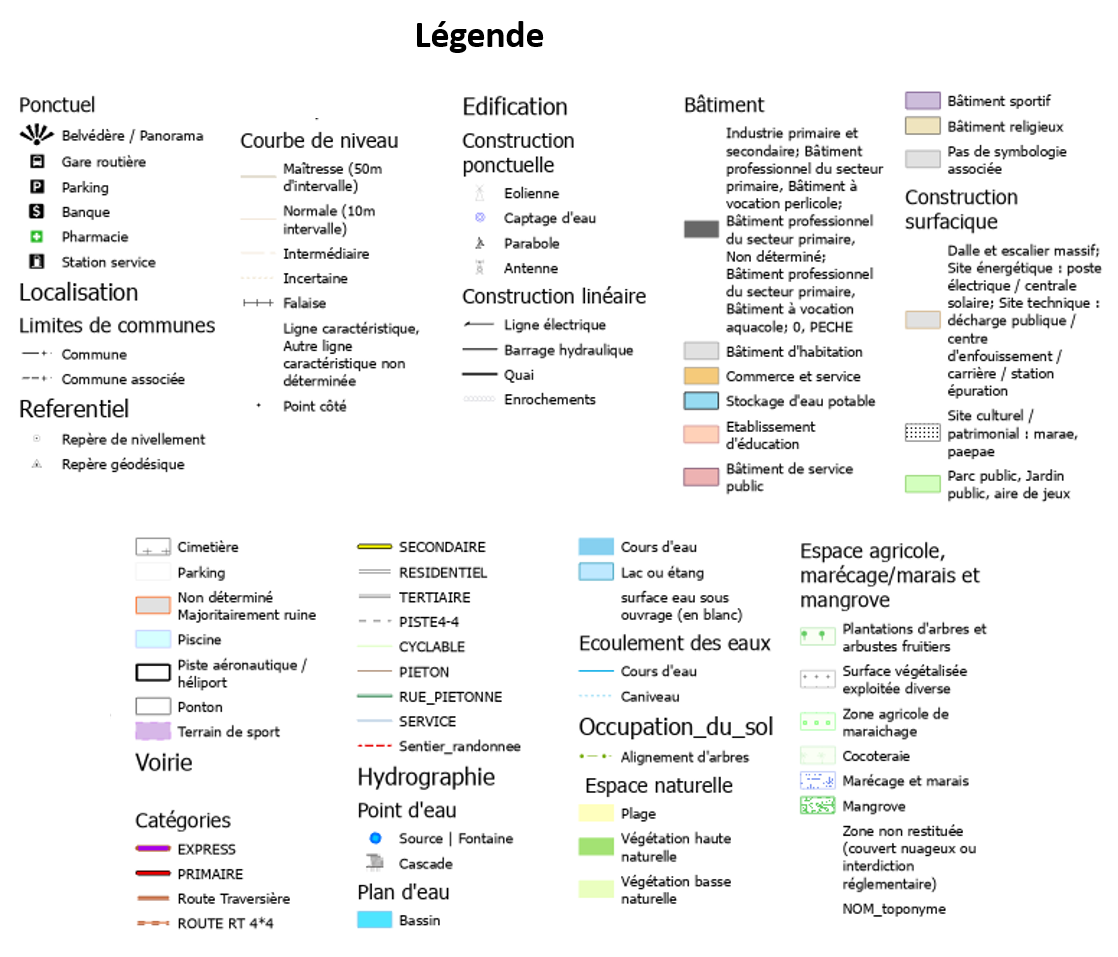
\includegraphics[width=\linewidth]{images/Annexes/Resultat/legende_15.png}
\caption{Légende de la carte au 1/15 000}
\label{15000_legende}
\end{figure}

\vspace{3cm}
\textsc{Commentaires sur la carte au 1/15 000 :}\\
Chemins de rando, etc, etc
\begin{figure}[!h]
\centering
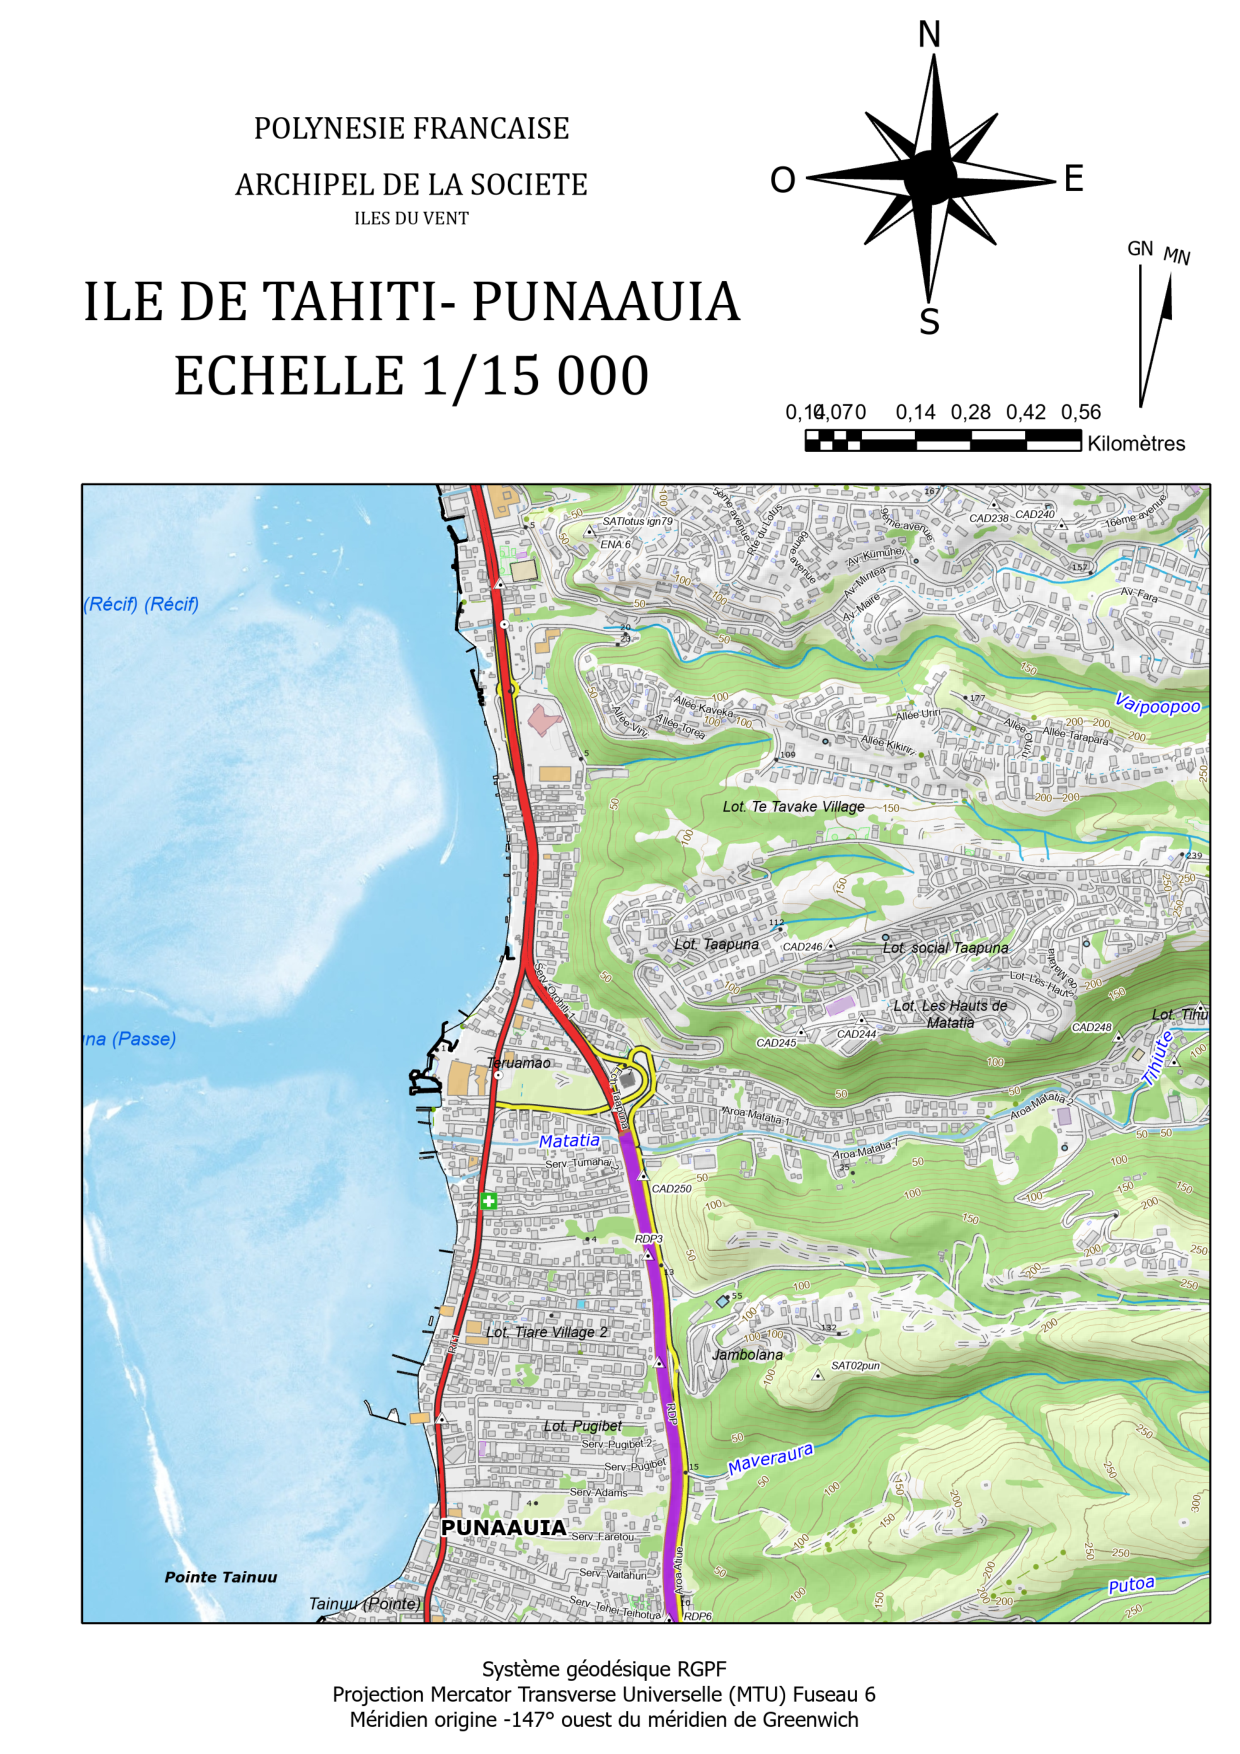
\includegraphics[width=\linewidth]{images/Annexes/Resultat/Carte_15000_A4.pdf}
\caption{Grossissement de la carte au 1/15 000 centrée sur Punaauia}
\label{15000_gros}
\end{figure}

\begin{sidewaysfigure}[!h]
\centering
\includegraphics[width=\linewidth]{images/Annexes/Resultat/Carte_15000_v2-bis.pdf}%
\caption{Echantillon résultat (version 2) }
\colorbox{yellow!10}{Echelle 1/15 000}
\label{15000 v2}% label for figure
\end{sidewaysfigure}

\clearpage
%%%%%%%%%%%%%%%%%%%%%%%%%%%
\begin{center}
    \Large
    \colorbox{green!10}{--------------\- Echelle 1/25 000 --------------\-}
\end{center}

\begin{figure}[!h]
\centering
\includegraphics[width=\linewidth]{images/Annexes/Resultat/legende_25.png}
\caption{Légende de la carte au 1/25 000}
\label{15000_legende}
\end{figure}

\vspace{3cm}
\textsc{Commentaires sur la carte au 1/25 000 :}\\

\begin{figure}[!h]
\centering
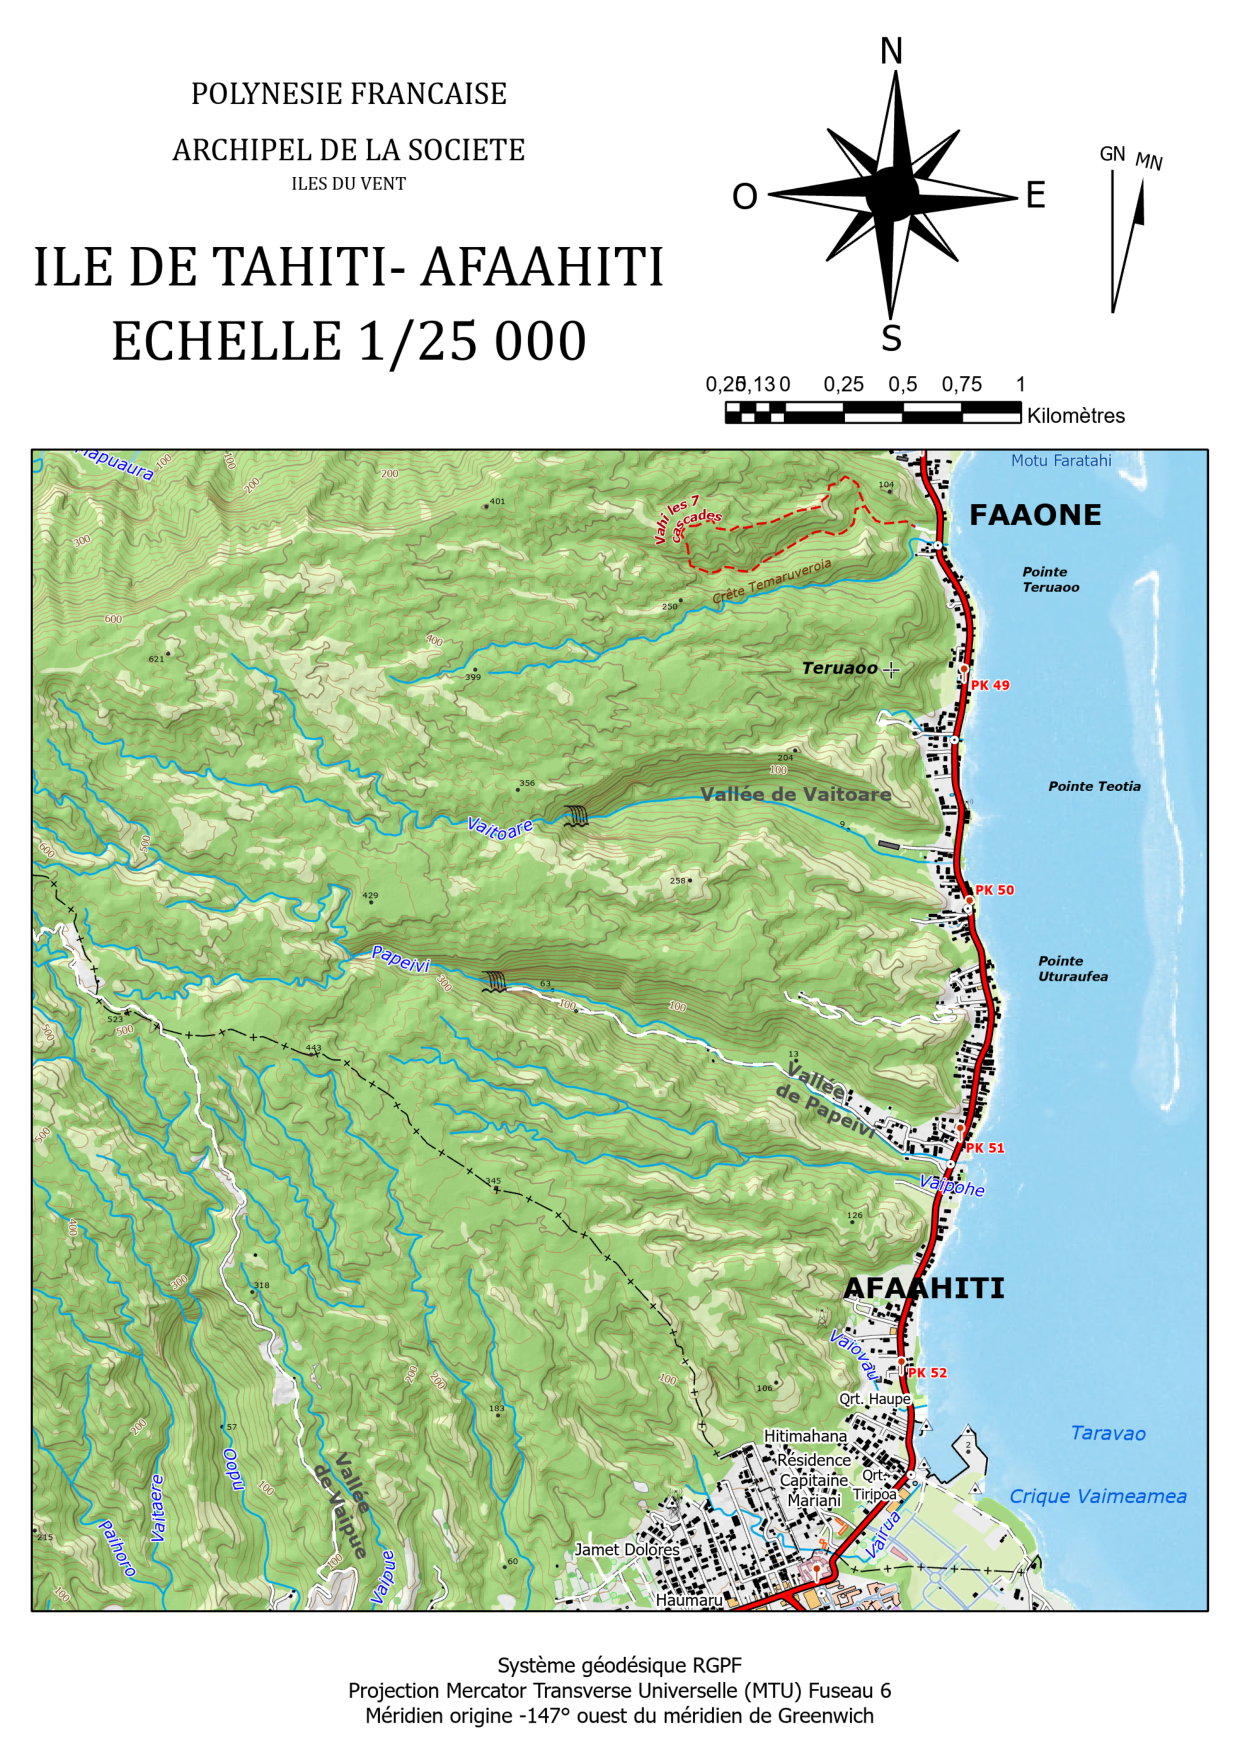
\includegraphics[width=\linewidth]{images/Annexes/Resultat/Carte_25000_A4.pdf}
\caption{Grossissement de la carte au 1/25 000 centrée sur ...}
\label{15000_gros}
\end{figure}

\begin{sidewaysfigure}[!h]
\centering
\includegraphics[width=\linewidth]{images/Annexes/Resultat/Carte_25000_v1-1.png}%
\caption{Echantillon résultat (version 4) }
\colorbox{green!10}{Echelle 1/25 000}
\label{15000 v2}% label for figure
\end{sidewaysfigure}

\clearpage
%%%%%%%%%%%%%%%%%%%%%%%%%%%%%%%%%%%%
\begin{center}
    \Large
    \colorbox{yellow!10}{--------------\- Echelle 1/50 000 --------------\-}
\end{center}

\begin{figure}[!h]
\centering
\includegraphics[width=\linewidth]{images/Annexes/Resultat/legende_50.png}
\caption{Légende de la carte au 1/50 000}
\label{15000_legende}
\end{figure}

\vspace{3cm}
\textsc{Commentaires sur la carte au 1/50 000 :}\\

\begin{figure}[!h]
\centering
\includegraphics[width=\linewidth]{images/Annexes/Resultat/Carte_50000_A4.pdf}
\caption{Grossissement de la carte au 1/50 000 centrée sur ...}
\label{15000_gros}
\end{figure}

\begin{sidewaysfigure}[!h]
\centering
\includegraphics[width=\linewidth]{images/Annexes/Resultat/Carte_50000_v1-1.png}%
\caption{Echantillon résultat (version 2) }
\colorbox{blue!10}{Echelle 1/15 000}
\label{15000 v2}% label for figure
\end{sidewaysfigure}

\clearpage

%%%%%%%%%%%%%%%%%%%%%%%%%%%%%%%%%%%%%%%%%%%%%%%%%%%%%%%%%%%%%%%%%%%%%%%%%%
%%%%%%%%%%%%%%%%%%%%%   ANNEXE XX  %%%%%%%%%%%%%%%%%%%%%%%%%%%%%%%%%%%%%%%%
%%%%%%%%%%%%%%%%%%%%%%%%%%%%%%%%%%%%%%%%%%%%%%%%%%%%%%%%%%%%%%%%%%%%%%%%%%
\annexe[Affichage pj]{ Affichage des images en pièces jointes sur ArcGIS Online}
\label{annexepj}


\definecolor{darkWhite}{rgb}{0.94,0.94,0.94}
 
\lstset{
    backgroundcolor=\color{darkWhite},
    breakatwhitespace=false,
    breaklines=true,
    captionpos=b,
    commentstyle=\color{red},
    deletekeywords={...},
    escapeinside={\%*}{*)},
    extendedchars=true,
    keepspaces=true,
    keywordstyle=\color{blue},
    language=C,
    morekeywords={*,...},
    showspaces=false,
    showstringspaces=false,
    showtabs=false,
    stepnumber=1,
    stringstyle=\color{gray},
    tabsize=1,
    title=Code Arcade pour l'affichage des pièces jointes dans ArcGIS Online,
}
\lstinputlisting{Code/arcade.js}
\clearpage


%%%%%%%%%%%%%%%%%%%%%%%%%%%%%%%%%%%%%%%%%%%%%%%%%%%%%%%%%%%%%%%%%%%%%%%%%%
%%%%%%%%%%%%%%%%%%%%%   ANNEXE XX  %%%%%%%%%%%%%%%%%%%%%%%%%%%%%%%%%%%%%%%%
%%%%%%%%%%%%%%%%%%%%%%%%%%%%%%%%%%%%%%%%%%%%%%%%%%%%%%%%%%%%%%%%%%%%%%%%%%
\annexe[Consommation des crédits ArcGIS pro pour l'export web]{ Consommation des crédits ArcGIS pro pour l'export web}
\label{crédits}



\clearpage	


%%%%%%%%%%%%%%%%%%%%%%%%%%%%%%%%%%%%%%%%%%%%%%%%%%%%%%%%%%%%%%%%%%%%%%%%%%
%%%%%%%%%%%%%%%%%%%%%   ANNEXE XX  %%%%%%%%%%%%%%%%%%%%%%%%%%%%%%%%%%%%%%%%
%%%%%%%%%%%%%%%%%%%%%%%%%%%%%%%%%%%%%%%%%%%%%%%%%%%%%%%%%%%%%%%%%%%%%%%%%%
\annexe[Présentation et fonctionnement du site web créé]{ Présentation du site web créé}

\begin{center}
    \Large
    Un portail des produits de la section topographie de la DAF
\end{center}


\begin{figure}[!h]
\centering
\includegraphics[width=\linewidth]{images/Annexes/siteweb1.png}
\caption{Capture d'écran du site web créé (1) }
\label{site1}
\end{figure}
Le principal outil développé durant ce stage est un portail (de type géoportail) topographique. Il est accessible dès l'entrée sur le site web, et peut être ouvert dans un onglet approprié. Il comprend les résultats des généralisation effectuées et exportées. Il peut être considéré comme un \textit{fond de carte} et peut être utilisé dans des applications thématiques.

Le site web est exploratoire. Il pourra être repris pour servir de plateforme utile à la diffusion des produits de la section topographie. Il permet aussi de voir les applications et les cartes thématiques. Parmi les applications, le site fait figurer celles concernant la diffusion des fiches géodésiques et de nivellement.

\begin{figure}[!h]
\centering
\includegraphics[width=\linewidth]{images/Annexes/siteweb2.png}
\caption{Capture d'écran du site web créé (2) }
\label{site2}
\end{figure}
\label{annexepj}



%%%%%%%%%%%%%%%%%%%%%%%%%%%%%%%%%%%%%%%%%%%%%%%%%%%%%%%%%%%%%%%%%%%%%%%%%%
%%%%%%%%%%%%%%%%%%%%%   ANNEXE XX  %%%%%%%%%%%%%%%%%%%%%%%%%%%%%%%%%%%%%%%%
%%%%%%%%%%%%%%%%%%%%%%%%%%%%%%%%%%%%%%%%%%%%%%%%%%%%%%%%%%%%%%%%%%%%%%%%%%
\annexe[Diagramme présentant le déroulement du projet]{ Diagramme présentant le déroulement du projet}
\label{gantt}

\begin{figure}[!h]
\centering
\includegraphics[width=\linewidth]{images/Annexes/gantt.png}%
\caption{Diagramme de déroulement du projet}
\label{gantt}
\end{figure}


Commentaires sur le diagramme...

\clearpage




\end{appendices} 

\end{document}